
\documentclass{upenndiss}
% The default font size is 12pt, but can be changed in the normal way:
% \documentclass[11pt]{upenndiss}
%
% The Penn guidelines allow smaller sizes, but be warned that the lines
% are too long for anything smaller than 12pt to be easily readable (see any
% introduction to designing text layouts).

% Add packages and definitions you want to use here:
\usepackage{times}
\usepackage{epsfig, bbm, subfigure} 
%\usepackage[mathbf,mathcal]{euler}
%\usepackage{pifont,epsfig}

\usepackage[
pdfauthor={Hari Sundar},
pdftitle={ Ph.D. Thesis },
pdfcreator={pdftex},
pdfsubject={Computer Aided Diagnosis of Cardiomyopathies},
pdfkeywords={Cardiomyopathy, CAD, registration},
pagebackref  = {true},
hyperindex = {true},
colorlinks = {true},
linkcolor = {blue},
pagecolor = {blue},
citecolor = {blue}
]{hyperref} 
%\usepackage{cite}

\usepackage{amsmath}
\usepackage{amsfonts}
\usepackage{amssymb}
%\usepackage{algorithmic}
%\usepackage{algorithm}

%%%%%%%%%% Start TeXmacs macros
\newcommand{\tmstrong}[1]{\textbf{#1}}
\newcommand{\tmmathbf}[1]{\ensuremath{\boldsymbol{#1}}}
\newcommand{\tmop}[1]{\ensuremath{\operatorname{#1}}}
\newenvironment{enumerateroman}{\begin{enumerate}[i.]}{\end{enumerate}}
%%%%%%%%%% End TeXmacs macros

\renewcommand{\div}{{\boldsymbol{\nabla}}}
\newcommand{\ul}{\underline}
\newcommand{\bea}{{\begin{eqnarray}}}
\newcommand{\eea}{{\end{eqnarray}}}
\newcommand{\beq}{{\begin{equation}}}
\newcommand{\eeq}{{\end{equation}}}
\newcommand{\tmccrap}{These results are based upon a test version of the
Thinking Machines Corporation software where the emphasis was on providing
functionality and the tools necessary to begin testing the CM-5 vector units.
This software release has not had the benefit of optimization or performance
tuning and, consequently, is not necessarily representative of the performance
of the full version of this software.}
\newcommand{\tafsm}{T\,\includegraphics[width=0.75em]{logo-star.eps}\,AFSM}

\newfont{\amsbold}{msbm10}
\newfont{\logobold}{logobf10 scaled\magstep2}
\newcommand{\real}{\mathbb{R}}
\newcommand{\assembly}{\mathop{\mbox{\logobold A}}}
\def\nsd{{n_\mathrm{sd}}}
\def\isd{{i_\mathrm{sd}}}
\def\nen{{n_\mathrm{en}}}
\def\nel{{n_\mathrm{el}}}
\def\iel{{i_\mathrm{el}}}
\def\nln{{n_\mathrm{ln}}}
\def\nq{{n_\mathrm{eq}}}
\def\nelem{{n_\mathrm{e}}}
\def\nnode{{n_\mathrm{n}}}
\def\ndf{{n_\mathrm{dof}}}
\def\idf{{i_\mathrm{dof}}}
\def\ned{{n_\mathrm{ed}}}
\def\nee{{n_\mathrm{ee}}}
\def\iee{{i_\mathrm{ee}}}
\def\nint{{n_\mathrm{int}}}
\def\nquad{{n_\mathrm{quad}}}
\def\iquad{{i_\mathrm{quad}}}
\def\neemax{n_\mathrm{ee\_max}}
\def\npes{{n_\mathrm{PEs}}}
\def\Ot{\Omega_t}
\def\Gt{\Gamma_t}
\def\On{\Omega_n}
\def\Gn{\Gamma_n}
\newcommand{\Reynolds}{\mathrm{Re}}
\newcommand{\Prandtl}{\mathrm{Pr}}
\newcommand{\Froude}{\mathrm{Fr}}
\newcommand{\Strouhal}{\mathrm{St}}
\def\sbn{{\pmb n}}
\def\sbt{{\pmb t}}
\def\sbb{{\pmb b}}
\newcommand{\ba}{\mathbf{a}}
\newcommand{\bb}{\mathbf{b}}
\newcommand{\bc}{\mathbf{c}}
\newcommand{\bd}{\mathbf{d}}
\newcommand{\be}{\mathbf{e}}
\newcommand{\force}{\mathbf{f}}
\newcommand{\bg}{{\boldsymbol{\mathit{g}}}}
\newcommand{\bh}{{\boldsymbol{\mathit{h}}}}
\newcommand{\bi}{\mathbf{i}}
\newcommand{\bj}{\mathbf{j}}
\newcommand{\bk}{\mathbf{k}}
\newcommand{\bm}{\mathbf{m}}
\newcommand{\bn}{\mathbf{n}}
\newcommand{\bp}{\mathbf{p}}
\newcommand{\bq}{\mathbf{q}}
\newcommand{\br}{\mathbf{r}}
\newcommand{\bs}{\mathbf{s}}
\newcommand{\bt}{\mathbf{t}}
\newcommand{\bu}{\mathbf{u}}
\newcommand{\bv}{\mathbf{v}}
\newcommand{\bw}{\mathbf{w}}
\newcommand{\bx}{\mathbf{x}}
\newcommand{\by}{\mathbf{y}}
\newcommand{\bz}{\mathbf{z}}
\newcommand{\bA}{\mathbf{A}}
\newcommand{\bB}{\mathbf{B}}
\newcommand{\bC}{\mathbf{C}}
\newcommand{\bD}{\mathbf{D}}
\newcommand{\bE}{\mathbf{E}}
\newcommand{\bF}{\mathbf{F}}
\newcommand{\bG}{\mathbf{G}}
\newcommand{\bH}{\mathbf{H}}
\newcommand{\bI}{\mathbf{I}}
\newcommand{\bJ}{\mathbf{J}}
\newcommand{\bK}{\mathbf{K}}
\newcommand{\bL}{\mathbf{L}}
\newcommand{\bM}{\mathbf{M}}
\newcommand{\bN}{\mathbf{N}}
\newcommand{\bO}{\mathbf{O}}
\newcommand{\bP}{\mathbf{P}}
\newcommand{\bQ}{\mathbf{Q}}
\newcommand{\bR}{\mathbf{R}}
\newcommand{\bS}{\mathbf{S}}
\newcommand{\bT}{\mathbf{T}}
\newcommand{\bU}{\mathbf{U}}
\newcommand{\bV}{\mathbf{V}}
\newcommand{\bW}{\mathbf{W}}
\newcommand{\bX}{\mathbf{X}}
\newcommand{\bY}{\mathbf{Y}}
\newcommand{\bZ}{\mathbf{Z}}
\newcommand{\zero}{\mathbf{0}}
\newcommand{\bxi}{{\boldsymbol{\xi}}}
\newcommand{\balpha}{{\boldsymbol{\alpha}}}
\newcommand{\bomega}{{\boldsymbol{\omega}}}
\newcommand{\bchi}{{\boldsymbol{\chi}}}
\newcommand{\btheta}{{\boldsymbol{\theta}}}
%\newcommand{\bChi}{{\boldsymbol{\Chi}}}
\newcommand{\bepsilon}{{\boldsymbol{\epsilon}}}
\newcommand{\bPsi}{{\boldsymbol{\Psi}}}
\newcommand{\bphi}{{\boldsymbol{\phi}}}
\newcommand{\bpi}{{\boldsymbol{\pi}}}
\newcommand{\design}{\balpha}
\def\but{{\bf u}_{,t}}
\def\bvt{{\bf v}_{,t}}
\def\ST{{{\cal S}^h_\bT}}
\def\VT{{{\cal V}^h_\bT}}
\def\SH{{{\cal S}^h_H}}
\def\VH{{{\cal V}^h_H}}
\def\Su{{{\cal S}^h_\bu}}
\def\Vu{{{\cal V}^h_\bu}}
\def\SU{{{\cal S}^h_\bU}}
\def\VU{{{\cal V}^h_\bU}}
\def\Sv{{{\cal S}^h_\bv}}
\def\Vv{{{\cal V}^h_\bv}}
\def\Sp{{{\cal S}^h_p}}
\def\Vp{{{\cal V}^h_p}}
\def\Sh{{{\cal S}^h_\phi}}
\def\Vh{{{\cal V}^h_\phi}}
\def\Sun{{(\Su)_n}}
\def\Vun{{(\Vu)_n}}
\def\SHn{{(\SH)_n}}
\def\VHn{{(\VH)_n}}
\def\SUn{{(\SU)_n}}
\def\VUn{{(\VU)_n}}
\def\Svn{{(\Sv)_n}}
\def\Vvn{{(\Vv)_n}}
\def\Spn{{(\Sp)_n}}
\def\Vpn{{(\Vp)_n}}
\def\Shn{{(\Sh)_n}}
\def\Vhn{{(\Vh)_n}}
\newcommand{\strain}{{\boldsymbol{\varepsilon}}}
\newcommand{\stress}{{\boldsymbol{\sigma}}}
\newcommand{\blambda}{{\boldsymbol{\lambda}}}
\renewcommand{\div}{{\boldsymbol{\nabla}}}
\newcommand{\sbg}{\bg}
\newcommand{\sbh}{\bh}
\newcommand{\btau}{\boldsymbol{\tau}}
\newcommand{\tauT}{{\tau_\mathrm{\scriptscriptstyle CONS}}}
\newcommand{\tauu}{{\tau_\mathrm{\scriptscriptstyle MOM}}}
\newcommand{\taup}{{\tau_\mathrm{\scriptscriptstyle CONT}}}
\newcommand{\taudc}{{\tau_\mathrm{\scriptscriptstyle DC}}}
\newcommand{\tauadv}{{\tau_\mathrm{\scriptscriptstyle ADV}}}
\newcommand{\tausupg}{{\tau_\mathrm{\scriptscriptstyle SUPG}}}
\newcommand{\taupspg}{{\tau_\mathrm{\scriptscriptstyle PSPG}}}
\newcommand{\taugls}{{\tau_\mathrm{\scriptscriptstyle GLS}}}
\newcommand{\tauglsa}{{\tau_\mathrm{\scriptscriptstyle GLS1}}}
\newcommand{\tauglsb}{{\tau_\mathrm{\scriptscriptstyle GLS2}}}
\newcommand{\oneovermu}{\frac{1}{2 \mu_{1}}}
\newcommand{\lamovermu}{\frac{\lambda}{2 \mu_{1}}}
\newcommand{\lsqovermu}{\frac{\lambda^{2}}{2 \mu_{1}}}
\newcommand{\hash}{{\includegraphics[width=0.1in]{x.ps}}}
\newcommand{\hashblue}{{\includegraphics[width=0.1in]{x-blue.ps}}}
\newcommand{\subhash}{{\includegraphics[width=0.06in]{x.ps}}}
\newcommand{\subhashblue}{{\includegraphics[width=0.06in]{x-blue.ps}}}
\newcommand{\upup}           {{\includegraphics[width=0.1in]{h.ps}}}
\newcommand{\upupblue}       {{\includegraphics[width=0.1in]{h-blue.ps}}}
\newcommand{\upupred}        {{\includegraphics[width=0.1in]{h-red.ps}}}
\newcommand{\upupmagenta}    {{\includegraphics[width=0.1in]{h-magenta.ps}}}
\newcommand{\subupup}        {{\includegraphics[width=0.1in]{h.ps}}}
\newcommand{\subupupblue}    {{\includegraphics[width=0.06in]{h-blue.ps}}}
\newcommand{\subupupred}     {{\includegraphics[width=0.06in]{h-red.ps}}}
\newcommand{\subupupmagenta} {{\includegraphics[width=0.06in]{h-magenta.ps}}}

\def\half{\frac{1}{2}}
\def\us{u^*}	\def\bus{{\bu^*}}	\def\buh{{\bu^h}}
\def\udiv{\bu\!\cdot \div}	\def\usdiv{\bus\!\cdot \div}
\def\uhdiv{\buh\!\cdot \div}
\def\divu{\div\!\cdot\!\bu}	\def\divus{\div\!\cdot\!\bus}
\def\divuh{\div\!\cdot\!\buh} \def\divv{\div\!\cdot\!\bv}
\def\vatwo{\left[\begin{array}{c}v_1^a\\v_2^a\end{array}\right]}
\def\ubtwo{\left[\begin{array}{c}u_1^b\\u_2^b\end{array}\right]}
\def\va3{\left[\begin{array}{c}v_1^a\\v_2^a\\v_3^a\end{array}\right]}
\def\ub3{\left[\begin{array}{c}u_1^b\\u_2^b\\u_3^b\end{array}\right]}
\def\fb3{\left[\begin{array}{c}f_1^b\\f_2^b\\f_3^b\end{array}\right]}
\def\rs#1{{r_{#1}^*}}	\def\brs#1{{{\bf r}_{#1}^*}}
\def\gradv3{\left[\begin{array}{ccc}
	v_{1,x_1}&v_{1,x_2}&v_{1,x_3}\\
	v_{2,x_1}&v_{2,x_2}&v_{2,x_3}\\
	v_{3,x_1}&v_{3,x_2}&v_{3,x_3}\\
\end{array}\right]}
\def\strainu3{\left[\begin{array}{ccc}
	2 u_{1,x_1}&u_{1,x_2}+u_{2,x_1}&u_{1,x_3}+u_{3,x_1}\\
	u_{2,x_1}+u_{1,x_2}&2 u_{2,x_2}&u_{2,x_3}+u_{3,x_2}\\
	u_{3,x_1}+u_{1,x_3}&u_{3,x_2}+u_{2,x_3}&2 u_{3,x_3}
\end{array}\right]}
\def\divstrainv3{\left[\begin{array}{c}
	2v_{1,x_1x_1}+v_{1,x_2x_2}+ v_{1,x_3x_3}+v_{2,x_1x_2}+ v_{3,x_1x_3}\\
	 v_{1,x_2x_1}+v_{2,x_1x_1}+2v_{2,x_2x_2}+v_{2,x_3x_3}+ v_{3,x_2x_3}\\
	 v_{1,x_3x_1}+v_{2,x_3x_2}+ v_{3,x_1x_1}+v_{3,x_2x_2}+2v_{3,x_3x_3}
\end{array}\right]}
\def\divstrainu3{\left[\begin{array}{c}
	2u_{1,x_1x_1}+u_{1,x_2x_2}+ u_{1,x_3x_3}+u_{2,x_1x_2}+ u_{3,x_1x_3}\\
	 u_{1,x_2x_1}+u_{2,x_1x_1}+2u_{2,x_2x_2}+u_{2,x_3x_3}+ u_{3,x_2x_3}\\
	 u_{1,x_3x_1}+u_{2,x_3x_2}+ u_{3,x_1x_1}+u_{3,x_2x_2}+2u_{3,x_3x_3}
\end{array}\right]}
\def\gradq3{\left[\begin{array}{c}q_{x_1}\\q_{x_2}\\q_{x_3}\end{array}\right]}
\def\gradp3{\left[\begin{array}{c}p_{x_1}\\p_{x_2}\\p_{x_3}\end{array}\right]}
%
% stress components
%
\def\Ts{{T^*}}	\def\bTs{{\bT^*}}	\def\bTh{{\bT^h}}	\def\bSh{{\bS^h}}
\def\S#1{{\tilde{S}_{#1}}}
\def\T#1{{\tilde{T}_{#1}}}	\def\Ts#1{{\tilde{T}_{#1}^*}}
%
\def\Sa{\left[\begin{array}{c}\S{1}^a\\\S{2}^a\\\S{3}^a\end{array}\right]}
\def\Tb{\left[\begin{array}{c}\T{1}^b\\\T{2}^b\\\T{3}^b\end{array}\right]}
%
% convective derivatives of stress
%
\def\dusT{\left( \div \bus \cdot \bT + \bT \cdot (\div \bus)^T\right)}
\def\duTs{\left( \div \bu \cdot \bTs + \bTs \cdot (\div \bu)^T\right)}
\def\duTh{\left( \div \buh \cdot \bTh + \bTh \cdot (\div \buh)^T\right)}
\def\dusTs{\left( \div \bus \cdot \bTs + \bTs \cdot (\div \bus)^T\right)}
\def\duS{\left( \div \bu \cdot \bS + \bS \cdot (\div \bu)^T\right)}
\def\duSh{\left( \div \buh \cdot \bSh + \bSh \cdot (\div \buh)^T\right)}
\def\dusS{\left( \div \bus \cdot \bS + \bS \cdot (\div \bus)^T\right)}
\def\triangledown{\mathchar"0235 }
\def\bDT{\overtriangle{\bT}}
\def\bDS{\overtriangle{\bS}}
%
% common VF expressions
%

\newcommand{\piola}{\mathcal{J}{\bf F^{-1}\tilde{T}F^{-T} }}
\newcommand{\rhou}{\left( \rho \bu \right)}
\newcommand{\rhoe}{\left( \rho e \right)}
\newcommand{\rhouu}{\left( \rho \bu \bu \right)}
\newcommand{\rhoeu}{\left( \rho e \bu \right)}
\newcommand{\drdt}{\frac{\partial \rho}{\partial t}}
\newcommand{\drudt}{\frac{\partial \rhou}{\partial t}}
\newcommand{\dredt}{\frac{\partial \rhoe}{\partial t}}
\newcommand{\dudt}{\frac{\partial \bu}{\partial t}}
\newcommand{\dudtsq}{\frac{\partial^2 \bu}{\partial t^2}}
\newcommand{\dUdt}{\frac{\partial \bU}{\partial t}}
\newcommand{\gradu}{\div \bu}
\newcommand{\gradut}{\left( \div \bu \right)^{T}}
\newcommand{\umag}{\|\bu\|}
\newcommand{\dudx}{\frac{\partial u_{1}}{\partial x_{1}}}
\newcommand{\dudy}{\frac{\partial u_{1}}{\partial x_{2}}}
\newcommand{\dudz}{\frac{\partial u_{1}}{\partial x_{3}}}
\newcommand{\dvdx}{\frac{\partial u_{2}}{\partial x_{1}}}
\newcommand{\dvdy}{\frac{\partial u_{2}}{\partial x_{2}}}
\newcommand{\dvdz}{\frac{\partial u_{2}}{\partial x_{3}}}
\newcommand{\dwdx}{\frac{\partial u_{3}}{\partial x_{1}}}
\newcommand{\dwdy}{\frac{\partial u_{3}}{\partial x_{2}}}
\newcommand{\dwdz}{\frac{\partial u_{3}}{\partial x_{3}}}

%------------------------------------------------------------
\newtheorem{algorithm}{\textbf{Algorithm}}
\newtheorem{acknowledgement}{Acknowledgement}
\newtheorem{axiom}{Axiom}
\newtheorem{lemma}{Lemma}
\newtheorem{proof}{Proof}
\newtheorem{case}{Case}
\newtheorem{claim}{Claim}
\newtheorem{conclusion}{Conclusion}
\newtheorem{condition}{Condition}
\newtheorem{conjecture}{Conjecture}
\newtheorem{criterion}{Criterion}
\newtheorem{example}{Example}
\newtheorem{exercise}{Exercise}

\newtheorem{notation}{Notation}
\newtheorem{problem}{Problem}

\newtheorem{remark}{Remark}
\newtheorem{prop}{Property}
\newtheorem{define}{Definition}
\newtheorem{solution}{Solution}
\newtheorem{summary}{Summary}
\numberwithin{equation}{section}
%\newenvironment{proof}{
%  \noindent\textbf{Proof}\ }{\hspace*{\fill}
%  \begin{math}\Box\end{math}\medskip}
%------------------------------------------------------------
\newcommand{\pe}{\psi}
\newcommand{\argmax}[1]{\ensuremath{\arg \,\underset{#1}{\max}\;}}
\def\d{\delta} 
\def\ds{\displaystyle} 
\def\e{{\epsilon}} 
\def\eb{\bar{\eta}}  
\def\enorm#1{\|#1\|_2} 
\def\Fp{F^\prime}  
\def\Kc{{\cal K}} 
\def\norm#1{\|#1\|} 
\def\wb{{\bar w}} 
\def\zb{{\bar z}} 


\def\bfE{\mbox{\boldmath$E$}}
\def\bfG{\mbox{\boldmath$G$}}




%%%%%%%%%%%%%%%%%%%  The title pages  %%%%%%%%%%%%%%%%%%%%%%%%%%%%%%%%

% Note: Use \protect\\ if you need a manual line break
%\title{A Really Clever Title: \protect\\ The Second Line of Your Title}
\title{Spatio-Temporal Deformation Analysis of Cardiac MR Images}

% Fill in here as appropriate.  Separate multiple names with \and  
\author{Hari Sundar}
\supervisor{Christos Davatzikos}
\gradchair{Susan Margulies}
\committee{George Biros \and Victor Ferrari \and Harold Litt \and Dinggang Shen}

% Change to \copyrighttrue if you want to generate a copyright page.
\copyrightfalse  
% \copyrightyear{2000}  % Defaults to the current year if undefined.

\department{Bioengineering}


%%%%%%%%%%%%%%%%%%%  Now for the front matter %%%%%%%%%%%%%%%%%%%%%%%%%

% Front matter elements are required to appear in a specific order.  In this
% section you define the parts of your front matter, and the style will
% automatically put them in the proper order.


% Declare the sections that you use.  Only Abstract is obligatory.  
%
\abstractfile{abstract}
\acknowledgementsfile{acknow}
% \dedicationfile{dedication}
% \prefacefile{preface}

% ALTERNATELY, if you have a really short Dedication (no more than one
% paragraph) you can place it in the main file, with the command
% \dedication{...}, INSTEAD of using \dedicationfile.
\dedication{\center
\textit{Quidquid id est,} \\
\textit{timeo Danaos et dona ferentes.} \\
\quad\quad-Vergil, Aeneid II.49}

\begin{document}
% The following command now generates all your starting pages:
\FrontMatter

\chapter{Introduction}
\label{intro}
 
\section{Motivation} 
According to WHO estimates, 16.7 million people around the world die of cardiovascular diseases (CVD) each year \cite{aha}. Of the total CVD deaths annually, about 8.6 million are of women. Heart attack and stroke deaths are responsible for twice as many deaths in women as all cancers combined. The US health care system is facing serious access and quality issues. The current access and quality issues will be compounded in the coming years by three factors that will serve to accelerate the rate of cardiovascular disease and its complications. 

First, aging of the population will undoubtedly result in a concomitant increase in the incidence of chronic diseases, including coronary artery disease, heart failure and stroke. Second, we are experiencing an explosive increase in the prevalence of obesity and type 2 diabetes and their related complications of hypertension, hyperlipidemia, and artherosclerotic vascular disease \cite{aha}. Finally, there is an alarming increase in unattended risk factors in the younger generations that will continue to fuel the cardiovascular epidemic for years to come. These factors include obesity and smoking. CVD is the leading cause of mortality in every region in the world except sub-Saharan Africa, and it is anticipated that cardiovascular disease will eclipse the present the current leader in that region, infectious disease, within the next few years. By 2020 the WHO estimates nearly 25 million CVD deaths worldwide. By 2020, cardiovascular diseases, injury and mental illnesses will be responsible for about one half of all deaths  and one half of all healthy years lost, worldwide. The socio-economic impact of cardiovascular disease is too great to be ignored. In 2004 the estimated direct and indirect cost of CVD was \$368.4 billion \cite{aha}.

It is noteworthy that the principal cardiovascular disorder responsible for the global rise in mortality is no longer rheumatic heart disease, but rather artherosclerotic vascular disease. Ischemic heart disease is the leading cause of death in the world, and cerebrovascular disease is the second leading cause \cite{aha}. It is often assumed that artherosclerosis is a disease of the affluent, industrialized countries. However, 80\% of these deaths occur in low-to-middle income countries of varying size like China, Russia, Poland, Mauritius, Argentina, and India \cite{wha}. In many countries, the need for care already outstrips the ability to provide it to its citizens. Throughout the world, even in economically advanced societies, there are deficiencies in preventive and acute care that might stem the tide of this epidemic. Because of these reasons, it is important to stop think of cardiovascular diseases as a rich-man's disease and start dealing with it as an epidemic. Consequently, it is extremely important to develop cheap, non-invasive early detection methods to be able to identify the onset of cardiovascular diseases and treat them before they cause excessive damage. 

There are a number of invasive and non-invasive procedures that are currently used for diagnosis of CVD \cite{merck}. To reduce trauma for the patient it is preferable to use non-invasive procedures. Important noninvasive techniques are plain radiography, radionucleotide imaging, positron emission tomography (PET), Magnetic Resonance Imaging (MRI) and Ultrasound \cite{merck}. Of these, MRI can provide much cardiac information during a single examination and may thus be more cost-effective than several other studies. In the last few years MRIs have become cheaper and more accessible and given the human and economic cost of CVD, it is important that high-risk populations be screened regularly for CVD. 

Cardiac diseases are characterized by both changes in the myocardial structure as well as changes in cardiac function. Consequently, it is important for any cardiac diagnosis method to consider both these aspects. Advances in MR Cine imaging methods have enabled us to acquire high-resolution 4D images of the heart that capture the structural and functional characteristics of individual hearts. However large inter and intra-observer variability in the interpretation of these images for the diagnosis of diffuse cardiomyopathies has been reported \cite{bluemke03}. Studies also suggest that standardizing acquisition protocols and objective analysis especially of regional myocardial function will help improve the accuracy and reduce inter-observer variability \cite{pattynama93}. This has created the need for sophisticated and highly automated image analysis methods, which can identify and precisely quantify subtle and spatially complex patterns of structural and functional changes in the heart. The main contribution of this thesis is the development of computational methods to characterize myocardial function from MR images.

Although the algorithms and methods developed as part of this work should apply in general to the whole class of diffuse cardiomyopathies, we restrict the scope to the characterization of Arrhythmogenic right ventricular cardiomyopathy (ARVC). Future work shall focus on how the methods developed as part of this work can be generalized to other diffuse cardiomyopathies.

%Therefore, MRI being a simple non-invasive method is an obvious choice for a screening test for CVDs. However, for this to happen in an effective manner it is important to develop diagnostic techniques that can quickly and effectively screen patients, making it faster and more cost effective compared to the current method of having specialists process all patients. 
%
%It takes an expert radiologist 20 minutes, on an average,to evaluate an MR scan of a patient for signs of CVD. This is generally the case for localized abnormalities like ischaemia. The diagnosis time can run into hours for non-localized CVDs like Arrhythmogenic right ventricular cardiomyopathy (ARVC) \cite{rvd}. Because of the sheer population that is at risk, it is important that these detection method's be automated, since detailed diagnosis by human experts is next to impossible. Therefore it is very important to develop Computer aided diagnosis (CAD) algorithms for cardiac diseases and have the experts further analyze the patients screened by the CAD algorithm for specific diagnosis and treatment. Even in these cases, the CAD algorithm can highlight abnormal behavior and make the job of the radiologist much easier. Developing the tools and algorithms for such a diagnosis method is the main goal of this work.

\section{Arrhythmogenic Right Ventricular Cardiomyopathy}

\subsection{Clinical Features and Relevance}

Arrhythmogenic right ventricular cardiomyopathy is generally accepted as the most common cause of sudden cardiac death in young patients, and despite over 25 years of study remains a poorly understood disease \cite{ferrari2003arv, thiene1988rvc}. Recent genetic studies have elucidated both autosomal dominant and recessive inheritance mechanisms \cite{paul2003gar}. Arrhythmogenic right ventricular cardiomyopathy (ARVC), also known as arrhythmogenic right ventricular dysplasia is characterized by progressive fibrofatty replacement of right ventricular myocardium, initially with typical regional and later global right and some left ventricular involvement, with relative sparing of the septum \cite{thiene1988rvc}. As the underlying pathophysiology of ARVC remains unknown, there is no consensus regarding a gold standard for diagnosis \cite{thiene2000pap}. Diagnosis of ARVC is based on presence of major and minor criteria that include structural, histological, electrocardiographic, arrhythmic, and genetic factors. At its early stages, the diagnosis of ARVC remains a clinical challenge. The different imaging modalities play a limited role, as there is no single non- invasive method that helps to establish or exclude this diagnosis.

\subsection{MR Imaging of ARVC}
While Magnetic Resonance imaging (MRI) findings were not included in the original Task Force criteria because of a lack of evidence of efficacy, it has been evaluated as a method for demonstration of the structural and functional abnormalities listed, including myocardial fatty replacement, RV dilation, wall thinning, and aneurysm formation, and evaluation of RV function \cite{bluemke03}. However, the diagnostic performance for detection of these abnormalities, as measured by sensitivity, specificity, and inter-observer variability remains somewhat uncertain. A recent single center study compared MR findings in 12 patients with definitive diagnosis of ARVC by Task Force criteria, with 10 age and sex matched controls \cite{tandri2003mri}. The study found evidence of intramyocardial fat in 75\% of the patients and none of the controls, a greater incidence of RV hypertrophy and statistically significant increases in quantitative measures of RV dimensions and decreases in RV function. In another study \cite{bluemke03}, 13 readers at multiple institutions reviewed images from MR evaluations of 7 patients with a diagnosis of ARVC by Task Force criteria, 6 controls, and 32 patients with suspected ARVC. While the presence of reported RV enlargement and other morphological abnormalities were significantly higher in the definitive ARVC patients, the percentages with reported intramyocardial fat were equal amongst the three groups. Overall diagnostic quality was poor and there was wide inter-observer variability for all parameters evaluated. Limitations of this study included non-standardization of MR acquisition techniques and criteria for interpretation, as well as lack of inclusion of functional cine images in the interpretations. The findings suggest that standardizing acquisition protocols and standardized, objective analysis especially of regional myocardial function will improve the accuracy and reduce variability.

\section{Assessing Myocardial Function}

Cardiomyopathies present themselves in different forms, both by structural changes like plaque formation, fat deposits, etc., and functional changes like variations in ventricular wall motion, ejection fraction, and perfusion. Both of these need to be extracted from the image before accurate diagnosis can be done. A lot of work has been done in feature extractors for structural characterizations of disease. This has focused primarily on extracting image features like intensities and gradients \cite{ intgrad}, moments \cite{ hammer,  moments}, Gabor features \cite{ manju96}, and local frequency representations \cite{ locfreq}. The problem with cardiomyopathies is that not all of them can be characterized by structural changes. Function at rest may be abnormal as a result of one of the spectrum of ischemic heart diseases (ischemia, infarction, hibernation) or of cardiomyopathy from other causes. During stress testing, new or worsening wall motion abnormalities are indicative of functionally significant coronary artery stenosis \cite{smart2000das}. In addition, wall motion imaging to detect regional contractile reserve is an accurate measure of myocardial viability, and the results can help guide coronary revascularization therapy. Characterizing cardiomyopathies based on both structural and functional changes will make the diagnosis algorithm more accurate and robust. Of course quantization of the myocardial wall motion represents a challenge in itself. 

Most clinical modalities used to image myocardial function evaluate passive wall motion (ventriculography) or wall thickening (echocardiography, gated single-photon emission computed tomography, or cine MR imaging). MR imaging also allows quantitative measurement of regional intramyocardial motion and, subsequently, strain, which can be more sensitive to wall motion abnormalities than is wall thickening. MR imaging methods for the quantification of intramyocardial wall motion can be loosely classified into two approaches, those relying on specially developed MR imaging protocols to help in the estimation of myocardial motion and those relying on image analysis techniques to extract motion estimates from MR Cine sequences.

\subsection{Specialized MR Protocols}
\subsubsection{MR Tagging}
MR Tagging was developed to provide non-invasive virtual markers inside the myocardium, which deform with myocardial motion \cite{ mrtag}. MR imaging and especially tagged MR are currently the reference modalities to estimate dense cardiac displacement fields with high spatial resolution. The deformation fields, as well as the derived motion parameters such as myocardial strain can be determined within an accuracy of 2mm x 2mm \cite{ Shi99, chenBook}. The primary disadvantage of tagging is the reduced spatial resolution of strain relative to the image spatial resolution. In tagging, after the displaced tag lines are detected \cite{ guttman94}, the displacement field can be estimated and intramyocardial strain can be computed in a variety of ways \cite{ mrtag}. With this approach, although strain may be interpolated to any desired spatial resolution, the fundamental spatial resolution of strain is nominally determined by the distance between the tag lines, which is typically several pixels. Tag detection has an additional disadvantage in that it typically requires substantial manual intervention and is therefore a time-consuming task. Harmonic phase analysis will likely obviate tag detection \cite{osman1999cmt}, but the spatial resolution of the resultant strain maps will not necessarily improve. The spatial resolution of strain maps obtained from tagged images after harmonic phase analysis is determined by the k-space filter of the analysis; in practice with single breath-hold acquisitions, the resolution has been relatively poor \cite{ garot00}. Additionally since the right ventricle (RV) is much thinner than the left ventricle (LV), it is difficult to place more than a single tag within the RV, making the estimation of RV motion extremely difficult and inaccurate. Since we are most interested in the characterizing RV function, tagging is not appropriate for our purpose.

\subsubsection{Phase Contrast Imaging}
The second approach is that of MR phase contrast imaging \cite{ mrphase}, which is based on the concept that spins that are moving in the same direction as a magnetic field gradient develop a phase shift that is proportional to the velocity of the spins. This information can be used directly to determine the velocity of the spins, or in the cardiac case the velocity of any point within the myocardium. The main problem with this approach is that four acquisitions have to be made for each heart, one the regular MR cine sequence and one phase contrast acquisition each for the velocity components in the x, y, and the z directions. Consequently, MR phase contrast imaging is not used much in a clinical setting. 

\subsubsection{DENSE and HARP}
Displacement-encoded imaging with stimulated echoes (DENSE) \cite{epstein2004dec} and harmonic phase imaging (HARP) \cite{osman1999cmt} employ 1-1 spatial modulation of magnetization to cosine modulate the longitudinal magnetization as a function of position at end diastole. Later in the cardiac cycle the cosine-modulated signal is sampled and used to compute myocardial strain from the signal phase. The sampled signal generally includes three distinct echoes:  a displacement-encoded stimulated echo, the complex conjugate of the displacement-encoded echo, and an echo arising from T1 relaxation. If the T1-relaxation and complex conjugate echoes are suppressed, then a phase image representing just the displacement-encoded echo can be reconstructed. However, data-acquisition in single-breath-hold DENSE MR imaging has been limited to only one cardiac phase. Multiple breath-hold DENSE produces images at multiple phases of the cardiac cycle, but the resolution has been poor and is fundamentally a 2D approach and the estimation of through-plane displacement has been poor. 

\subsection{Extracting motion from MR Cine images}
An alternate approach is to estimate myocardial motion from MR Cine sequences. MR Cine images in a clinical setting at sub millimeter resolutions (in-plane), with slice thickness in the range of 6-10mm. The temporal resolution varies between 25-70ms. A lot of work has been done in extracting cardiac motion fields from MR and Ultrasound image sequences \cite{ Shi99,  ledesma01, McE00, Papa01, perperidis04,  Song91,  Wang01}. These can be classified into two main categories. The first approach uses segmentation of the myocardial wall, followed by geometric and mechanical modeling using active contours or surfaces to extract the displacement field and to perform the motion analysis \cite{ Shi99,  Papa01,  Wang01}. For matching two contours or surfaces, curvatures are frequently used to establish initial sparse correspondences, followed by the dense correspondence interpolation in other myocardial positions by regularization or mechanical modeling \cite{ Shi99, McE00}. The lack of distinct landmarks on the myocardial wall makes it difficult to estimate the wall motion based on surface tracking. In addition this approach is very sensitive to the accuracy with which the myocardium can be segmented. Also it performs poorly in regions within the myocardium, and manages to only align the myocardial boundaries. The other approach uses energy-based warping or optical flow techniques to compute the displacement of the myocardium \cite{ ledesma01,  perperidis04,  Song91}. Perperidis et al. \cite{ perperidis04} use a regular grid with a B-spline basis to model the deformation and use normalized mutual information as the similarity metric which is calculated over the whole image. One of the major shortcomings of these approaches is that the transformation estimated as a result of the registration is not unique and in fact does not necessarily conform to the underlying myocardial motion. The same algorithm can give different estimates of motion for different initial guesses and different parameters. The problem arises since these methods attempt to maximize the image similarity with only a smoothness constraint on the transformation. Since there can be many transformation that can map an image onto another (especially sparsely sampled ones as in the case of MR Cines) there is no guarantee that the estimated transformation is the correct one \cite{ Cachier:MICCAI:01,  Cachier-JMIV-2004}. These methods estimate motion by evolving the current estimate of motion under the action of external image forces (image similarity) and internal forces which constrain the regularity of the motion (smoothness). Such regularizers work well with respect to noise removal but they do not incorporate a priori knowledge of the underlying cardiac motion. Incorporating a biomechanically-inspired model for the myocardium has the potential for a more accurate motion estimation \cite{mcculloch1998cbh}. Functional models of the heart are direct computational models, designed to reproduce in a realistic manner the cardiac activity, often requiring high computational costs and the manual tuning of a very large set of parameters. Such methods can be computationally prohibitive for our purposes, and we instead select a level of modeling compatible with reasonable computing times and involving a limited number of parameters. Such simplifications add additional modeling errors, but our hypothesis is that in spite of these modeling errors the estimated motion fields shall be more accurate than those obtained from approaches not incorporating a priori knowledge. A detailed and thorough review of cardiac image registration methods can be found in \cite{ makela02} and a general review of image registration methods can be found in \cite{ Zitova03}. 

\section{Biomechanical Modeling of the Heart}

\section{Contributions}

\section{Organization of this Thesis}
\include {hammer}
\chapter{Mechanical Model of the Heart}
\label{sec:model}

\section{Introduction}
In this chapter we describe the anatomical structure of the human heart and describe how we translate that information to build a simple mechanical model of the heart. This mechanical model is used to constrain the problem of cardiac motion estimation, as shall be explained in detail in Section \ref{chap:inverse}. The heart is a complicated system, with an electro-mechanical system responsible for the activation and contraction of the heart muscles. Modeling of cardiac anatomy, electrophysiology and mechanics is an active research field. A comprehensive review of the field can be found in \cite {sachse04}. Muscle fiber orientations need to be considered while modeling cardiac electro-mechanics. The diffusion properties of the muscle fibers play an important role in the propagation of cardiac activation current. Similarly the force generated by the muscles is along the fiber direction. Therefore knowledge of the diffusion tensor or at least the fiber orientations is very important for modeling purposes, especially if the models are patient specific. It is not possible to obtain diffusion tensor images in vivo currently, and as a result most modeling approaches use synthetic data for the fiber orientations. These models for fiber orientations are very simple and capture only the basic trends in the orientation. Since our goal is to estimate the motion of the heart, we ignore the electrical stimulation that activates the heart muscles and develops the forces in the myo-fibers. Instead we solve for the forces directly, and only model the mechanical aspects of the heart. For this we solve a linear elasticity equation at all the fibers. The model parameters are the fiber orientations, and the material properties. We first describe how these parameters are obtained, followed by the governing equations for the model.

\section{Anatomical Structure of the Heart}
Modeling of cardiac anatomy, electrophysiology, and mechanics is very important for understanding the complicated interactions that take place between different anatomical structures. This knowledge helps us to understand the mechanisms of heart failure, and can help devise ways to prevent and cure such pathologies. A large number of cardiac pathologies occur because of problems with the electro-mechanical system within the heart. Consequently, a lot of active research is being carried out in this field.  A comprehensive review of the field can be found in \cite{mackerle2005fem, sachse04}. 


The walls of the heart are composed of cardiac muscle, called myocardium. It consists of four compartments: the right and left atria and ventricles. The heart is oriented so that the anterior aspect is the right ventricle while the posterior aspect shows the left atrium. The left ventricular free wall and the septum are much thicker than the right ventricular wall. This is logical since the left ventricle pumps blood to the systemic circulation, where the pressure is considerably higher than for the pulmonary circulation, which arises from right ventricular outflow. Since a muscle fiber can contract only in one direction, the heart structure is complex, to succeed at pumping the blood. Anatomically, to achieve this, the muscle walls of the ventricles and the atria are composed of a single helically folded muscular structure as can be seen in Figure \ref{grays_1}. The cardiac muscle fibers are divided into four groups \cite{gray18}: Two groups of fibers wind around the outside of both ventricles. Beneath these fibers a third group winds around both ventricles. Beneath these fibers a fourth group winds only around the left ventricle. 

\begin{figure}[!hbtp]
\begin{center}
\includegraphics[width=0.4\textwidth]{images/grays_3}
\includegraphics[width=0.34\textwidth]{images/grays_2} 
\caption{\em \small Fiber orientations in the Human Heart showing the helical structure of the muscles (from \cite{gray18})}
\label{grays_1}
\end{center}  
\end{figure} 

\section{Mechanical Modeling}

\[
	\rho \ddot{\bf u} - \mu\Delta{\bf u} + (\lambda+\mu)\nabla {\bf div~} {\bf u} = {\bf f}R({\bf u})\vec{\eta_0}
	\]	

We model the heart as a linear elastic solid occupying a bounded region $\omega$, with Dirichlet boundary conditions. Its displacement is described by 

\begin{equation}
\nabla \cdot \left[\lambda({\bf x})\left(\div \cdot {\bf U} \right) {\bf I} + \mu({\bf x})  \left( \div {\bf U} + (\div {\bf U} )^T \right) \right] + {\bf f}R({\bf U})\bN_0 = 0  \mbox{~~~~in~} \omega \mbox{,~~~~} {\bf U}  = {\bf g} \mbox{~~~~on~} \gamma.
\label{e-linear}
\end{equation}

Here ${\bf u}$ is the displacement field, and $\lambda({\bf x})$ and $\mu({\bf x})$ are the Lam\'{e} parameters which are related to the Young's Modulus $E({\bf x})$ and Poisson's ratio $\nu({\bf x})$. $\bR(\bU)$ is the rotational component of the local displacement field, by which the fiber orientation $\bN_0$ must be rotated. To solve (\ref{e-linear}) we embed $\omega$ in a regular domain $\Omega$. We use trilinear finite elements to discretize (\ref{e-linear}), and piecewise constant functions for $\lambda,\nu$.  The Poisson ratio $\nu({\bf x})$ varies between $0$ for a fully compressible material to $0.5$ for a fully incompressible material. When considering soft tissue deformations, the value of the Poisson ratio given for many tissue classes borders on the limit of incompressibility\footnote{As $\nu$ approaches 0.5, commonly used displacement-based finite element implementations suffer from the so-called locking effect.  We use underintegration for the $\nabla \cdot {\bf u}$ term in (\ref{e-linear}); see \cite{Hughes87} for details.}. Gladilin~\cite{Gladilin2003} studies the sensitivity of the Poisson ratio on the displacement field obtained via an incompressible formulation and a compressible formulation. The results indicate that Poisson ratio does not affect the solution significantly.

\subsection{Linear Elastodynamics}

We assume that the MR image occupies the region $\Omega \in \mathbb{R}^3$ in its reference state (end-diastole) at time $t=0$. The boundary $\Gamma=\partial\Omega$ has the outward unit normal given by $\bn$, the displacement vector is represented by $\bu$, and the velocity by $\bv$. The myocardium is assumed to be made of an elastic material and is subject to body force $\force$ per unit volume.

The strong form of the equations of linear elastodynamics are written as:
\begin{eqnarray}
\rho\dudtsq &=& \div\cdot\stress + \force \qquad \mbox{in} ~\Omega\times]0,T[, \\
\stress \bn &=& 0, \qquad\qquad~~~~ \mbox{in} ~\Gamma\times]0,T[, \nonumber\\
\bu(t=0) &=& \bu_0, \qquad\qquad~~ \mbox{in} ~\Omega \nonumber\\
\dot{\bu}(t=0) &=& \bv_0, \qquad\qquad~~ \mbox{in} ~\Omega \nonumber
\end{eqnarray}
where $\bu_0$ is the initial displacement, $\bv_0$ is the initial velocity, $\stress$ is the stress tensor and $\div\cdot\stress$ denotes the divergence of $\stress$. Assuming that the material is isotropic and homogeneous, one may express the stress tensor as
\begin{equation}
\label{eq:stressstrain}
\stress = \lambda~\mbox{tr}~\strain\bI + 2\mu\strain,
\end{equation}
in terms of the Lam\'{e} constants $\lambda$ and $\mu$, the identity tensor $\bI$, and the infinitesimal strain tensor $\strain$. The strain is defined as
\begin{equation}
\label{eq:strain}
\strain := \frac{1}{2}\left[ \gradu + \gradut \right] := \div_s\bu~,
\end{equation} 
where $\gradu$ is the gradient operator expessed in Cartesian component form as
\[
[\gradu] = \left[ \begin{array}{c}u_1\\u_2\\u_3\end{array}\right] 
\left[\begin{array}{ccc} \dfrac{\partial}{\partial x} & \dfrac{\partial}{\partial y} & \dfrac{\partial}{\partial z} \end{array}\right] =
\left[
\begin{array}{ccc} 
u_{1,1} & u_{1,2} & u_{1,3} \\
u_{2,1} & u_{2,2} & u_{2,3} \\
u_{3,1} & u_{3,2} & u_{3,3}
\end{array}
\right] ~.
\]
Using equation (\ref{eq:strain}), the components of the strain tensor are
\[
[\strain] = \left[
\begin{array}{ccc} 
u_{1,1} & \frac{1}{2}(u_{1,2}+u_{2,1}) & \frac{1}{2}(u_{1,3}+u_{3,1}) \\
\frac{1}{2}(u_{1,2}+u_{2,1}) & u_{2,2} & \frac{1}{2}(u_{2,3}+u_{3,2}) \\
\frac{1}{2}(u_{1,3}+u_{3,1}) & \frac{1}{2}(u_{2,3}+u_{3,2}) & u_{3,3}
\end{array}
\right] ~.
\]

%% Variational formulation
Let $\bw$ denote the variations, and $\bw \in \mathcal{V}$ the variation space.
Then the weak form can be written as
\begin{equation}
\int_{\Omega} \bw\cdot(\rho\dudtsq-\div\cdot\stress -\force)~d\Omega + \int_{\Gamma} \bw\cdot\stress\bn~d\Gamma = 0.
\end{equation}
Using the Einsteinian summation convention, we can write it as,

\begin{eqnarray}
  0 & = & \int_{\Omega} w_i ( \rho u_{i, t t} - \sigma_{i j, j} - f_i )~d\Omega + \int_{\Gamma} w_i \sigma_{ij} n_j~d \Gamma \nonumber\\
	& = & \int_{\Omega} w_i \rho_i u_{i, t t}~d\Omega - 	
	\left(	\int_{\Omega} w_i\sigma_{ij,j}~d\Omega \right) -
  \int_{\Omega} w_i f_i~d\Omega + \int_{\Gamma} w_i \sigma_{ij} n_j~d\Gamma \nonumber\\
  & = & \int_{\Omega} w_i \rho_i u_{i, t t}~d\Omega - 	
	\left(	\int_{\Omega} (w_i\sigma_{ij})_{,j}~d\Omega - \int_{\Omega} w_{i,j}\sigma_{ij}~d\Omega \right) -
  \int_{\Omega} w_i f_i~d\Omega + \int_{\Gamma} w_i \sigma_{ij} n_j~d\Gamma \nonumber\\
	& = & \int_{\Omega} w_i \rho_i u_{i, t t}~d\Omega - 	
	\left( \int_{\Gamma} w_i \sigma_{ij} n_j~d\Gamma - \int_{\Omega} w_{i, j}\sigma_{ij}~d\Omega \right) -
  \int_{\Omega} w_i f_i~d\Omega + \int_{\Gamma} w_i \sigma_{ij} n_j~d\Gamma \nonumber\\
  & = & \int_{\Omega} w_i \rho_i u_{i, t t}~d\Omega + \int_{\Omega} w_{( i, j )} \sigma_{ij}~d\Omega - \int_{\Omega} w_i f_i~d\Omega,
\end{eqnarray}
where use is made of integration by parts and the divergence theorem. It follows that,
\begin{equation}
\label{eq:weakForm}
\int_{\Omega} \bw\cdot\rho\ddot{\bu} ~d\Omega - \int_{\Omega}\div_s\bw:\stress ~d\Omega = \int_{\Omega} \bw\cdot\force ~d\Omega ~,
\end{equation}
where $\div_s\bw:\stress$ denotes the contraction of the tensors $\div_s\bw$ and $\stress$, expressed in component form as $\div_s\bw:\stress=w_{i,j}\sigma_{ij}$.

Equation (\ref{eq:weakForm}) motivates us to define the following bilinear forms:
\begin{eqnarray}
  a (\bw,\bu) & = & -\int_{\Omega}\div_s\bw:\stress ~d\Omega, \label{eq:bilinear} \\ %= \int_{\Omega} w_{( i, j )} \sigma_{ij}~d\Omega\\
  (\bw,\force) & = & \int_{\Omega} \bw\cdot\force ~d\Omega, ~\mbox{and}~ \\ %= \int_{\Omega} w_i f_i~d\Omega \nonumber\\
  (\bw, \rho \ddot{\bu} ) & = & \int_{\Omega} \bw\cdot\rho\ddot{\bu} ~d\Omega. % = \int_{\Omega} w_i \rho u_{i, t t} d \Omega \nonumber
\end{eqnarray}
The corresponding weak formulation can be written as:

Given $\force, \bu_0 \tmop{and} \bv_0$, find $\bu( t ) \in \mathcal{S}_t, t \in [ 0, T ]$,
such that for all $\bw \in \mathcal{V}$, such that 
\begin{eqnarray}
  (\bw, \rho \ddot{\bu} ) + a (\bw,\bu) &
  = & (\bw,\force), \\
  (\bw, \rho \bu( 0 ) ) & = & (\bw, \rho \bu_0 ), \nonumber\\
  (\bw, \rho \dot{\bu} ( 0 ) ) & = & (\bw, \rho \tmmathbf{v}_0 ) \nonumber.
\end{eqnarray}

In order to simply the expressions, we express the components of tensorial quantities such as $\div_s\bw$ and $\stress$ in vector form. In particular we define the strain vector as,  

\[ 
	\strain(\bu) = 
	\left\{ \begin{array}{c}
	\epsilon_{11} \\ \epsilon_{22} \\ \epsilon_{33} \\
	2\epsilon_{12} \\ 2\epsilon_{23} \\ 2\epsilon_{31}
	\end{array} \right\}  =
	\left\{ \begin{array}{c}
     u_{1, 1}\\
     u_{2, 2}\\
     u_{3, 3}\\
     u_{2, 3} + u_{3, 2}\\
     u_{1, 3} + u_{3, 1}\\
     u_{1, 2} + u_{2, 1}
   \end{array} \right\} 
\]

Likewise, the stress tensor can be written in vector form as,

\[
\stress = \left\{ \begin{array}{c}
	\sigma_{11} \\ \sigma_{22} \\ \sigma_{33} \\
	\sigma_{12} \\ \sigma_{23} \\ \sigma_{31} \end{array} \right\} 
\]

The stress-strain law (\ref{eq:stressstrain}) can be written using the vector convention as
\begin{equation}
\label{ref:stressstrainMat}
[\stress] = [\bD][\strain],
\end{equation} 

where $[\bD]$ is a ($6\times6$) elasticity matrix such that
\begin{equation}
  \bD= \left[ \begin{array}{cccccc}
    \lambda + 2 \mu & \lambda & \lambda & 0 & 0 & 0\\
    \lambda & \lambda + 2 \mu & \lambda & 0 & 0 & 0\\
    \lambda & \lambda & \lambda + 2 \mu & 0 & 0 & 0\\
    0 & 0 & 0 & \mu & 0 & 0\\
    0 & 0 & 0 & 0 & \mu & 0\\
    0 & 0 & 0 & 0 & 0 & \mu
  \end{array} \right]
\end{equation}

Since the matrix $[\bD]$ is always symmetric, it follows that the integrand of the bilinear form in (\ref{eq:bilinear}) can be written with the aid of (\ref{ref:stressstrainMat}) as

\[
\div_s\bw:\stress = [\strain(\bw)][\bD][\strain(\bu)] := \strain(\bw)\cdot\bD\strain(\bu) ,
\]
which shows that the bilinear form in (\ref{eq:bilinear}) in indeed symmetric. 

\subsection{Semidiscrete Galerkin formulation of elastodynamics}

Given $\force, \bu_0, \tmop{and} \dot{\bu_0}$, find $\bu^h =\bv^h
+\tmmathbf{g}^h,\bu^h ( t ) \in \mathcal{S}_t^h$, such that for all
$\bw^h \in \mathcal{V}^h$,
\begin{eqnarray}
  (\bw^h, \rho \ddot{\tmmathbf{v}}^h ) + a
  (\bw^h,\tmmathbf{v}^h ) & = & (\bw^h, f ) 
- (\bw^h, \rho \ddot{\tmmathbf{g}}^h ) - a (\bw^h,\tmmathbf{g}^h ) \nonumber\\
  (\bw^h, \rho \tmmathbf{v}^h ( 0 ) ) & = & (\bw^h, \rho
  \bu_0 ) - (\bw^h, \rho \tmmathbf{g}^h ( 0 ) ) \nonumber\\
  (\bw^h, \rho \dot{\tmmathbf{v}}^h ( 0 ) ) & = & (\bw^h,
  \rho \dot{\bu}_0 ) - (\bw^h, \rho \dot{\tmmathbf{g}}^h ( 0
  ) ) 
\end{eqnarray}
The representations of $\bw^h,\tmmathbf{v}^h \tmop{and}
\tmmathbf{g}^h$ are given by
\begin{eqnarray}
  \bw^h (\tmmathbf{x}, t ) = w_i^h (\tmmathbf{x}, t )\tmmathbf{e}_i &
  = & \sum_{A \in \eta - \eta_{q_i}} N_A (\tmmathbf{x}) c_{i A} ( t
  )\tmmathbf{e}_i \nonumber\\
  \tmmathbf{v}^h (\tmmathbf{x}, t ) = v_i^h (\tmmathbf{x}, t )\tmmathbf{e}_i &
  = & \sum_{A \in \eta - \eta_{g_i}} N_A (\tmmathbf{x}) d_{i A} ( t
  )\tmmathbf{e}_i \nonumber\\
  \tmmathbf{g}^h (\tmmathbf{x}, t ) = g_i^h (\tmmathbf{x}, t )\tmmathbf{e}_i &
  = & \sum_{A \in \eta_{g_i}} N_A (\tmmathbf{x}) g_{i A} ( t )\tmmathbf{e}_i 
\end{eqnarray}
Substituting (14) into (13) we get, (ignoring $\tmmathbf{e}_i, \tmop{and}
\tmmathbf{e}_j$ for clarity,

\begin{eqnarray*}
& & \left( \sum_{A \in \eta_{\tmop{int}}} N_A (\tmmathbf{x}) c_{i A} ( t ),
   \sum_{B \in \eta_{\tmop{int}}} N_B (\tmmathbf{x}) \rho \ddot{d_{}}_{j B} (
   t ) \right) + a \left( \sum_{A \in \eta_{\tmop{int}}} N_A (\tmmathbf{x})
   c_{i A} ( t ), \sum_{B \in \eta_{\tmop{int}}} N_B (\tmmathbf{x}) d_{i B} (
   t ) \right) \\
&=& \left( \sum_{A \in \eta_{\tmop{int}}} N_A (\tmmathbf{x}) c_{i
   A} ( t ),\force \right) + \left( \sum_{A \in \eta_{\tmop{int}}} N_A
   (\tmmathbf{x}) c_{i A} ( t ),\mathfrak{h} \right)_{\Gamma} -   
   \left( \sum_{A \in \eta_{\tmop{int}}} N_A (\tmmathbf{x}) c_{i A} ( t ),
   \sum_{B \in \eta_{q_i}} N_B \rho \ddot{g}_{i B} ( t ) \right) \\
&-& a\left(  \sum_{A \in \eta_{\tmop{int}}} N_A (\tmmathbf{x}) c_{i A} ( t ), \sum_{B
   \in \eta_{q_i}} N_B g_{i B} ( t ) \right) 
\end{eqnarray*}

This gives us a set of $3 \eta_{\tmop{int}} = 3 ( \eta - \eta_{q_i} )$
equations, where $\eta$ is the total number of nodes,
\begin{eqnarray*}
& & \sum^{n_{\tmop{dof}}}_{j = 1} \sum_{B \in \eta_{\tmop{int}}} ( N_A
  \tmmathbf{e}_i, N_B \tmmathbf{e}_j ) \rho \ddot{d}_{j B} ( t ) + \sum_{j =
  1}^{n_{\tmop{dof}}} \sum_{B \in \eta_{\tmop{int}}} a ( N_A \tmmathbf{e}_i,
  N_B \tmmathbf{e}_j ) d_{j B} ( t ) \\
&=& ( N_A \tmmathbf{e}_i,\force) + ( N_A \tmmathbf{e}_j,\mathfrak{h})_{\Gamma}  - \sum^{n_{\tmop{dof}}}_{j = 1}
  \sum_{B \in \eta_{q_j}} ( N_A \tmmathbf{e}_i, N_B \tmmathbf{e}_j ) \rho
  \ddot{g}_{j B} ( t ) - \sum_{B \in \eta_{q_j}} a ( N_A \tmmathbf{e}_i, N_B
  \tmmathbf{e}_j ) g_{j B} ( t )
\end{eqnarray*}


For the case of homogeneous dirichlet boundary conditions, $\tmmathbf{g}= 0,
\tmop{and} \eta_{q_i} = 0$, therefore (10) reduces to a set of $3 \eta$
equations in $3 \eta$ unknowns,
\begin{equation}
  \sum^{n_{\tmop{dof}}}_{j = 1} \sum_{B \in \eta} ( N_A \tmmathbf{e}_i, N_B
  \tmmathbf{e}_j ) \rho \ddot{d}_{j B} ( t ) + \sum^{n_{\tmop{dof}}}_{j = 1}
  \sum_{B \in \eta} a ( N_A \tmmathbf{e}_i, N_B \tmmathbf{e}_j ) d_{j B} ( t )
  = ( N_A \tmmathbf{e}_i,\force) + ( N_A
  \tmmathbf{e}_i,\mathfrak{h})_{\Gamma}
\end{equation}
In order to derive the mass matrix, the global stiffness matrix and the force
vector, we need to specify the global ordering of equations. This shall be
explained in detail later, for now we assume we have a function
{\tmstrong{id(i,A)}} that takes the degree of freedom and the global node
number as input and returns the global equation number. Using this we can
write the {\tmstrong{matrix problem}} as:

%\begin{tabular}{|c|}
%  \hline \\
%  \begin{eqnarray}
%    \tmmathbf{M} \ddot{\tmmathbf{d}} +\tmmathbf{K} \tmmathbf{d} & = &
%    \force \nonumber\\
%    \tmmathbf{d}( 0 ) & = & \tmmathbf{d}_0 \nonumber\\
%    \dot{\tmmathbf{d}} ( 0 ) & = & \dot{\tmmathbf{d}}_0 
%  \end{eqnarray}
%  \hline
%\end{tabular}

where the mass matrix,
\[ \tmmathbf{M}= \bigwedge_{e = 1}^{n_{\tmop{el}}} (\tmmathbf{m}^e ) \]
here, $\bigwedge$is the matrix assembly operator, and the elemental mass
matrix, $\tmmathbf{m}^e$ is given in terms of nodal submatrices as,
\begin{eqnarray}
  \tmmathbf{m}^e & = & \left[ m_{p q}^e \right] \nonumber\\
  m_{p q}^e & = & \delta_{i j} \int_{\Omega_e} N_a \rho N_b d \Omega 
\end{eqnarray}
\begin{notation}
  In all these definitions, $n_{\tmop{en}}$ is the number of element nodes,
  which for the trilinear hexahedral element is 8; $n_{\tmop{ed}}$ is the
  number of element degrees of freedom per node, which is 3 in our case. Also
  $n_{\tmop{ee}}$ stands for the number of element equations, which is
  $n_{\tmop{ed}} n_{\tmop{en}}$.
\end{notation}

\begin{notation}
  For the elemental mass matrix, $1 \leqslant p, q \leqslant n_{\tmop{ee}} =
  n_{\tmop{ed}} n_{\tmop{en}}$. Therefore in our case the elemental mass
  matrix shall be $24 \times 24$. For the nodal submatrices, indices  $p =
  n_{\tmop{ed}} ( a - 1 ) + i$, and $q = n_{\tmop{ed}} ( b - 1 ) + j$. 
\end{notation}

Similarly, the stiffness matrix can be written as,
\begin{eqnarray}
  \tmmathbf{K} & = & \bigwedge_{e = 1}^{n_{\tmop{el}}} (\tmmathbf{k}^e )
  \nonumber\\
  \tmmathbf{k}^e & = & \left[ k_{p q}^e \right] \nonumber\\
  k_{p q}^e & = & \tmmathbf{e}_i^T \int_{\Omega_e} \tmmathbf{B}_a^T
  \tmmathbf{D} \tmmathbf{B}_a d \Omega \tmmathbf{e}_j 
\end{eqnarray}
where the matrices $\tmmathbf{D}$ was defined earlier (7) and $\tmmathbf{B}_a$
is given by,
\begin{eqnarray*}
  \tmmathbf{B}_a & = & \left[ \begin{array}{ccc}
    N_{a, x} & 0 & 0\\
    0 & N_{a, y} & 0\\
    0 & 0 & N_{a, z}\\
    0 & N_{a, z} & N_{a, y}\\
    N_{a, z} & 0 & N_{a, x}\\
    N_{a, y} & N_{a, x} & 0
  \end{array} \right]
\end{eqnarray*}
We can now proceed to write the right hand side of our equation, i.e., the
force vector. This can be written as,
\begin{eqnarray}
  \force( t ) & = & \force_{\tmop{nodal}} ( t ) +
  \bigwedge_{e = 1}^{n_{\tmop{el}}} (\force^e ( t ) ) \nonumber\\
  \force^e & = & \{ f_p^e \} \nonumber\\
  f_p^e & = & \int_{\Omega_e} N_a f_i d \Omega +
  \int_{\Gamma_{\mathfrak{h}_i}} N_a \mathfrak{h}_i d \Gamma 
\end{eqnarray}
Also, we get the expressions for the initial conditions as,
\begin{eqnarray*}
  \tmmathbf{d}_0 & = & \tmmathbf{M}^{- 1} \bigwedge_{e =
  1}^{n_{\tmop{el}}} ( \hat{\tmmathbf{d}}^e )\\
  \hat{\tmmathbf{d}}^e & = & \{ \hat{d}_p^e \}\\
  \hat{d}_p^e & = & \int_{\Omega_e} N_a \rho u_{0 i} d \Omega\\
  \dot{\tmmathbf{d}_0} & = & \tmmathbf{M}^{- 1} \bigwedge_{e =
  1}^{n_{\tmop{el}}} ( \widehat{\dot{\tmmathbf{d}^e}}^{} )\\
  \widehat{\dot{\tmmathbf{d}^e}} & = & \{ \widehat{\dot{d_{}^{}}} _p^e \}\\
  \widehat{\dot{d_{}^{}}} _p^e & = & \int_{\Omega_e} N_a \rho \dot{u}_{0 i} d
  \Omega
\end{eqnarray*}
Of course under the assumption that the heart is stationary at the end of
diastole, which is our reference frame, $u_{0 i} = \dot{u_{0 i}} = 0$ and
therefore $\tmmathbf{d}_0 = \dot{\tmmathbf{d}_{}}_0 =\tmmathbf{0}$.

\subsection{Solving the forward problem: Newmark Scheme}

In order to solve the forward problem, we use the Newmark method. We use the
average acceleration or trapezoidal rule, which uses the values $\beta = 1 / 4
\tmop{and} \gamma = 1 / 2$. We first define the predictors,
\begin{eqnarray}
  \tilde{\tmmathbf{d}}_{n + 1} & = & \tmmathbf{d}_n + \Delta t\tmmathbf{v}_n +
  \frac{\Delta t^2}{4} \tmmathbf{a}_n \nonumber\\
  \tilde{\tmmathbf{v}}_{n + 1} & = & \tmmathbf{v}_n + \frac{\Delta t}{2}
  \tmmathbf{a}_n 
\end{eqnarray}
We can determine the acceleration at the next time instant by solving,
\begin{equation}
  \left( \tmmathbf{M}+ \frac{\Delta t^2}{2} \tmmathbf{K} \right)
  \tmmathbf{a}_{n + 1} =\force_{n + 1} -\tmmathbf{K}
  \tilde{\tmmathbf{d}}_{n + 1}
\end{equation}
We solve this to obtain $\tmmathbf{a}_{n + 1}$, and then obtain the values of
$\tmmathbf{d}_{n + 1} \tmop{and} \tmmathbf{v}_{n + 1}$ using the correctors
\begin{eqnarray}
  \tmmathbf{d}_{n + 1} & = & \tilde{\tmmathbf{d}}_{n + 1} + \frac{\Delta
  t^2}{4} \tmmathbf{a}_{n + 1} \nonumber\\
  \tmmathbf{v}_{n + 1} & = & \tilde{\tmmathbf{v}}_{n + 1} + \frac{\Delta t}{2}
  \tmmathbf{a}_{n + 1} 
\end{eqnarray}

\subsubsection{Imposing boundary conditions.} 

\begin{figure}
  \centering  
  \includegraphics[width=0.5\textwidth]{images/mat_prop}
  \caption{\em \small The material properties and boundary conditions for the cardiac model. We set the stress, $\sigma = 0$, at the boundary $\Gamma$. Different Lam\'{e}  parameters are selected for the myocardium ($\lambda_1, \mu_1$), blood ($\lambda_2, \mu_2)$, the lungs ($\lambda_3, \mu_3)$ and for bone ($\lambda_4, \mu_4)$ }
 \label{matprop}
\end{figure}	

We consider the input data as defined by the MR/DTI image to define the regular domain $\Omega$. The boundary conditions are exactly prescribed on the six faces of the cuboid, $\Gamma$, are simply set to have zero stress, i.e., $\sigma = 0$. One important issue is the accurate integration of the elements that overlap in the inhomogeneity transition. For simplicity we have used voxelized material	properties even in the case of exact geometry information. Within the regular domain $\Omega$, different material properties are assigned based on the tissue type. We currently consider the myocardium ($\lambda_1, \mu_1$), blood ($\lambda_2, \mu_2$), the lungs ($\lambda_3, \mu_3$) and bone ($\lambda_4, \mu_4$). These are shown in Figure \ref{matprop}.

%(This is easy to modify with small computational costs).  The second case, ( case (c) in figure \ref{fig:alg}) corresponds to {\bf Dirichlet	conditions} which we approximate by a constrained optimization approach in which the Dirichlet conditions are imposed through either Lagrange multipliers, or a simpler penalty formulation	\cite{babuska-73}. The latter corresponds to having a very stiff material surrounding the target domain. The nonzero case is treated	by linearity: we construct a smooth function $w(x)$ such that $w(x) = g(x)$ on $\gamma$, where $g(x)$ are the specified boundary conditions. We represent the solution of $L u(x) = f(x)$ as $u = w	+ v$, and we solve for $L v(x) = f - L w(x)$ with homogeneous Dirichlet conditions ($L$ is the linear elasticity operator); $w(x)$ is constructed using a triangulation, or a level-set representation of the boundary.  {\bf Neumann conditions} are imposed using a soft material ( case (d) in fig. \ref{fig:alg}). If $\sigma$ is the imposed stress, the weak form of a Neumann problem (for the Laplacian operator for simplicity) is given by $\int_{\omega}\nabla u\cdot\nabla v=\int_{\gamma}\sigma v$, for all $v$. Using the characteristic function $\chi_{\omega}$ (its value is one inside $\omega$ and zero outside), the weak form becomes $\int_{\Omega}\chi_{\omega}\nabla u\cdot \nabla v = \int_{\gamma}\sigma v$. We can approximate $\chi_{\omega}$ by using a soft material outside $\omega$.

%More complex boundary conditions are not as straightforward. The case in which a Dirichlet condition is specified in the normal direction, and a Neumann condition on the tangent plane can be approximated by anisotropic fictitious materials which are stiff in the normal direction and soft in the tangential direction. Mixed conditions in which part of the boundary is Neumann and part is Dirichlet require more complicated material selection for $\Omega\backslash\omega$. The convergence rates are suboptimal for the jumps in the material properties, whereas the boundary conditions are satisfied only approximately---for the Neumann and Dirichlet cases.

\subsubsection{Multigrid acceleration.} Multigrid methodologies have revolutionized scientific computation, especially for elliptic partial differential equations. Multigrid solvers consist of three main components: the smoother that reduces the algebraic residual at each level, and the restriction and prolongation operators for intergrid transfers \cite{brandt-77}. Typical smoothers are stationary iterative solvers, e.g. Gauss-Seidel. The multigrid method works very well for constant coefficient PDEs, but slows down for strongly variable coefficient problems.  In \cite{alcouffe-brandt-etal-81} a multigrid method for high-contrast materials is presented but is quite restrictive: material property jumps have to align with the grid. Algebraic multigrid is another alternative, but it requires an assembled matrix; this is costly and incompatible with our goals. Here we use a different approach. We are not using the multigrid algorithm to solve, but rather {\em to precondition} a Krylov method. Furthermore the smoothers within the multigrid iteration consist of a number of preconditioned Krylov iterations. We are using a Conjugate Gradient solver both to drive the overall residual, and as a smoother at each level. For high-contrast materials it is important to precondition the smoothers too; we have found that a simple damped Jacobi method suffices to obtain good algorithmic scalability. We use classical full-weighting and linear interpolation intergrid transfer operators. Extensive numerical tests have demonstrated robustness on high contrast inhomogeneities.  Our code is developed on top of PETSc~\cite{petsc-home-page}, a scientific computing library from Argonne National Laboratory.	

\section{Diffusion Tensor Imaging}

Diffusion tensor Imaging (DTI) is a technique to measure the anisotropic diffusion properties of biological tissues within the sample. This allows us to noninvasively infer the structure of the underlying tissue. Diffusion properties allow the classification of different types of tissues and can be used for tissue segmentation and detecting tissue orientations. The principal eigenvector of the diffusion tensor is known to align with fiber tracts in the brain \cite{pierpaoli96} and in the heart \cite{scollan98}. Heart fibers reconstructed from cardiac DTI are shown in Figure \ref{fibers-dti}.

Diffusion tensors describe the diffusion properties of water molecules. In tissues diffusion properties are dictated by the cell structure of the tissue. Since cell membranes are selectively permeable, water molecules can move easily within a cell, but their diffusion across the membrane is limited. Thus diffusion properties of the tissue reflect the shape and orientation of the cells. For the specific case of elongated cells like the cardiac muscles, the diffusion will be maximum along the primary axis of the muscle, which also happens to be the direction along which maximum strain is developed.

\begin{figure}
\begin{center}
\includegraphics[width=0.4\textwidth]{images/fibers3}
\caption{\em \small Heart fiber orientation in the human heart, obtained from diffusion tensor imaging}
\label{fibers-dti}
\end{center}  
\end{figure} 

Diffusion is measured through a diffusion coefficient, which is represented as a symmetric second order tensor:

\begin{equation}
\label{eq:dt}
{\bf D} = \left( 				
\begin{array}{ccc}
D_{xx} & D_{xy} & D_{xz} \\
D_{yx} & D_{yy} & D_{yz} \\	
D_{zx} & D_{zy} & D_{zz}
\end{array}
          \right)
\end{equation}
The 6 independent values of the tensor elements vary continuously with the spatial location in the tissue.

Eigenvalues $\lambda_i$ and eigenvectors ${\bf e}_i$ of the diffusion tensor (\ref{eq:dt}) can be found
as a solution to the eigenvalue problem:
\[
{\bf De}_i = \lambda_i{\bf e}_i
\]
Since the tensor is symmetric, its eigenvalues are always real numbers, and the eigenvectors are orthogonal and form a basis. Geometrically, a diffusion tensor can be thought of as an ellipsoid with its three axes oriented along these eigenvectors, with the three semiaxis lengths proportional to the square root of the eigenvalues of the tensor.

% Using the ellipsoidal interpretation, one can classify the diffusion properties of a tissue according to the shape of the ellipsoids, with extended ellipsoids corresponding to regions with strong linear diffusion (long, thin cells), flat ellipsoids to planar diffusion, and spherical ellipsoids to regions of isotropic media (such as fluid filled regions like the ventricles). The quantitative classification can be done through the coefficients $c_l$, $c_p$, $c_s$ corresponding to linear, planar and spherical diffusion.
%\begin{eqnarray*}
%c_l &=& \frac{\lambda_1 - \lambda_2}{\lambda_1 + \lambda_2 + \lambda_3} \\
%c_l &=& \frac{2(\lambda_2 - \lambda_3)}{\lambda_1 + \lambda_2 + \lambda_3} \\
%c_l &=& \frac{3\lambda_1}{\lambda_1 + \lambda_2 + \lambda_3}
%\end{eqnarray*}

The heart fibers have strong linear diffusion %($\lambda_1 >> \lambda_2 \approx \lambda_3)$ 
and are oriented along the principal eigenvector, ${\bf e}_1$ \cite{tseng99, scollan98}. Therefore if we need fiber orientations for a specific subject, then computing the principal direction of the diffusion tensor is sufficient. However, {\em in vivo} acquisition of cardiac DTI is not possible using current scanners and acquisition protocols. Consequently, we use an alternate strategy and map the diffusion tensors from a template image onto the subject. The procedure for warping DTIs from a template onto a subject is described in the following section.

\section {Warping Diffusion Tensors from template to subjects}

We have MR images for both the subject and the template. The diffusion tensor data is available only for the template. We use a very high dimensional elastic registration technique \cite{hammer} to estimate the deformation that warps the template to the subject space. We use this deformation field to map the fibers from the template to the subject. It is more complicated to warp tensor fields than it is to warp scalar images. This is because the tensor must be reoriented on each image voxel, in addition to a voxel displacement that is implied by the deformation field. This is achieved by finding the rotational component of the deformation field. We test the effectiveness of the tensor remapping algorithm by comparing the mapped tensors with the ground truth diffusion tensors for 19 canine datasets\footnote{CCBM, Johns Hopkins University}. The method of computing the transformation between the two geometries and the tensor reorientation algorithm are now described.

\subsection{Deformable Image Registration}

Image warping for deformable registration has received a great deal of attention during the past decade \cite{Zitova03}. In the present work we used a very-high-dimensional elastic transformation procedure in 3D volume space, referred to as the hierarchical attribute matching mechanism for elastic registration (HAMMER) method, which is determined from T1-weighted images and applied on the coregistered DT image of the template. This approach uses image attributes to determine point correspondences between an individual image and a template, which resides in the stereotaxic space and is the subject for which we have the diffusion tensors. A hierarchical sequence of piece-wise smooth transformations is then determined, so that the attributes of the warped images are as similar as possible to the attributes of the target. Relatively fewer, more stable attributes are used in the initial stages of this procedure, which helps avoid local minima, a known problem in high-dimensional transformations. The details of this algorithm can be found in \cite{hammer}.


\subsection{Tensor Reorientation}
It is a simple matter to warp a scalar image by a known spatial transformation. The image value from a particular voxel is transferred, via the displacement field of the spatial transformation, to a voxel in the target image. Typically, some sort of interpolation must also be applied. However, a more complex procedure is required to warp tensor fields, especially when the tensor estimates are noisy. We use an approach similar to that proposed by Xu et al \cite{xu03}.

If we know the direction, ${\bf v}$, of the fiber on voxel with coordinates ${\bf x}$, we can readily find the rotated version, ${\bf v}'$, of ${\bf v}$, according to the warping transformation. If ${\bf R}$ is the matrix that rotates ${\bf v}$ to ${\bf v'}$, then ${\bf R}$ should be applied to the respective tensor measurement. However, in practice we do not know ${\bf v}$. In fact, this is precisely what we would like to estimate. We only have a noisy orientation of $v$, which is the principal direction (PD) of the corresponding tensor measurement. One could use that PD in place of ${\bf v}$, as proposed in \cite{alex01}. However, that makes the approach vulnerable to noise, since the PD is only a noisy observation, and could be quite different from the true underlying fiber orientation. 

Assuming that we know the probability distribution function (PDF), $f({\bf v})$, of the fiber direction ${\bf v}$, we can find the rotation matrix, $\tilde{\bf R}$ which minimizes the expected value of $\|{\bf v' -Rv} \|^2$ over all orthonormal matrices ${\bf R}$:

\begin{eqnarray*}
\tilde{\bf R} &=& \mathop{\arg \min}_{\bf R} E\{\|{\bf v' -Rv} \|^2\}\\
&=& \mathop{\arg \min}_{\bf R} \int_{\bf v} pdf({\bf v}) \|{\bf v' -Rv} \|^2 d{\bf v}
\end{eqnarray*}

This problem can be solved by the Procrustean estimation \cite{golub83}, if a number of random samples, ${\bf v}$, are drawn from the PDF, and their respective rotated versions, ${\bf v'}$, are found by the rotation that the warping field applies to ${\bf v}$. If we arrange these vectors ${\bf v'}$ and ${\bf v}$ to form the columns of the matrices ${\bf A}$ and ${\bf B}$, respectively, then $\tilde{\bf R}$ is found by minimizing:
\[
	\left\|{\bf A} - {\bf R}\cdot{\bf B}\right\|_2^2 = \left\|{\bf A}\right\|_2^2 + \left\|{\bf B}\right\|_2^2 + 2\sum_i\sigma_i({\bf A}\cdot{\bf B}^T)
\]

where $\sigma_i(\bM)$ are the singular values of matrix ${\bf M}$. $\tilde{\bf R}$ can be determined via a singular value decomposition of ${\bf A \cdot B}$.

\begin{eqnarray*}
{\bf A}\cdot{\bf B}^T &=& {\bf V}\cdot\Sigma\cdot {\bf W}^T \\
\tilde{\bf R} &=& {\bf V}\cdot{\bf W}^T 
\end{eqnarray*}

More details on the algorithm and the estimation of the PDF can be found in \cite{xu03}.

\section{Results and Validation}

We used canine DTI datasets obtained from Center for Cardiovascular Bioinformatics and Modeling, Johns Hopkins University and acquired at the National Institue of Health, to validate the effectiveness of our diffusion tensor remapping algorithm. A total of $19$ canine subjects were scanned, of which $12$ subjects were normal, and $7$ had cardiac failure. The scans were performed {\em in vitro} after the hearts were harvested. Each heart was placed in an acrylic container filled with Fomblin, a perfluoropolyether (Ausimon, Thorofare, NJ). Fomblin has a low dielectric effect and minimal MR signal, thereby increasing contrast and eliminating unwanted susceptibility artifacts near the boundaries of the heart.  The long axis of the hearts was aligned with the $z$ axis of the scanner.  Images were acquired with a 4-element knee phased array coil on a 1.5 T GE CV/I MRI Scanner (GE, Medical System, Wausheka, WI) using an enhanced gradient system with 40 mT/m maximum gradient amplitude and a 150 T/m/s slew rate.

Since only the long axis of the heart was aligned with the $z$ axis of the scanner, we first need to correct for rotation about the $z$ axis. We picked one of the normal canine hearts as the template, and performed affine registration to warp the remaining subjects onto the template space. The diffusion tensors for these subjects were also rotated by the rotational component of the affine transform. We then perform the elastic registration using HAMMER to estimate the transformation that maps the template to the subject space. This transformation is then used to warp and reorient the diffusion tensors of template onto the subject. The quality of the mapping is measured by computing the angle between the principal direction of the mapped tensor and the principal direction of the ground truth obtained from the subject's DTI. This is shown in Figure \ref{fig:dot}.

The error in the fiber orientations is further demonstrated on one slice in Figure \ref{fig:pd_both}, by comparing the original fibers (in red) and the mapped fibers (in blue). Our method was able to successfully map the fibers for healthy as well as for failing canine hearts. The percentage of voxels where the error in the principal directions is less than $10^\circ$ is shown in Figure \ref{fig:graph}. We evaluate an error of less than $10^\circ$ since it is close to the average error obtained from DTI imaging \cite{scollan98} and histological measurements\cite{streeter73}. We also compare this with the error by using a synthetic model to estimate fiber orientations. The synthetic fiber orientations were produced by varying the elevation angle between the short axis plane and the fiber between $+90^\circ$ and $-90^\circ$ from the endocardium to the epicardium. Similar synthetic models have been used in \cite{sachse04, sermesant04}.

\begin{figure}
\begin{center}
\framebox{
%\includegraphics[width=0.4\textwidth]{images/dot_prod} 
\includegraphics[width=0.4\textwidth]{images/dot}}
\caption{\em \small The angle between the mapped principal direction with the actual principal direction, in degrees. The image is overlaid on a segmentation of the heart based on the fractional anisotropy } 
\label{fig:dot}
\end{center}  
\end{figure} 

%Also in order to verify whether the fiber orientations are sufficiently close for fiber tracking purposes, we created a checkerboard DTI using the original and mapped DTIs.  We performed fiber tracking on this checkerboard DTI and the resulting fibers are shown in Figure Y, alongside the fibers obtained from only the original DTI. 
%The method was able to successfully map the fibers for healthy as well as for failing canine hearts. The percentage of voxels where the error the principal directions is less than $10^\circ$ is shown in Figure \ref{fig:graph}. 

%The plot also shows the error introduced in the same heart where a synthetic model was used to estimate the fiber orientations. The synthetic fiber orientations were produced by varying the elevation angle between the short axis plane and the fiber between $+90^\circ$ and $-90^\circ$ from the endocardium to the epicardium. Similar synthetic models have been used in CITE metaxas, Semersant, sachse.

The method was able to map the fibers accurately for both healthy as well as for failing hearts that had left bundle branch blocks. Although, the percentage of voxels having an error of less than $10^\circ$ was lower in the failing hearts as compared to the healthy ones, we observe that most of these errors are in the vicinity of the block as expected, and the fiber orientations away from the bundle branch block were similar to that observed in healthy patients. Therefore, our method should perform better for other pathologies like ventricular hypertropy and infarction, since it has been shown that the muscle fiber orientations are not affected significantly by hypertrophy and myocardial infarction\cite{walker05}. 

\begin{figure}
\begin{center}
%\includegraphics[width=0.4\textwidth]{images/dot_prod} 
\includegraphics[width=0.5\textwidth]{images/pd_mapped_dti_2} 
\includegraphics[width=0.395\textwidth]{images/pd_mapped_dti_3} 
\caption{\em \small The principal directions of the original DT are shown in blue. The mapped principal directions are shown in red. The glyphs are overlaid on a segmentation of the heart based on the fractional anisotropy of the mapped DT}
\label{fig:pd_both}
\end{center}  
\end{figure} 

\begin{figure}
\begin{center}
%\includegraphics[width=0.4\textwidth]{images/dot_prod} 
\includegraphics[width=0.8\textwidth]{images/graph} 
\caption{\em \small The percentage of voxels having less than $10^\circ$ error in the principal directions after mapping }
\label{fig:graph}
\end{center}  
\end{figure} 

%\usepackage{amsmath}
%\usepackage{amsfonts}
%\usepackage{amssymb}
%\usepackage{bbm, subfigure, appendix}

%}}}

%{{{ introduction

\chapter{Octree Meshing}
\label{chap:octree}

Spatial decompositions of the $d$-dimensional cube have important
applications in scientific computing: they can be used as algorithmic
foundations for adaptive finite element methods \cite{becker00,kim02},
adaptive mesh refinement methods \cite{griebel98, popinet03}, and
many-body algorithms \cite{greengard89, aluru02, shangHua98, warren92,
ying04, ying03}. The earliest examples of tree-based spatial
decompositions of $\mathcal{R}^n$ can be traced to the use of {\em
binary space partitions} \cite{ fuchs83, fuchs80, schumaker69}.
Binary space partitioning (BSP) is a method for recursively
subdividing a space into convex sets by hyperplanes. This subdivision
gives rise to a representation of the space by means of a tree data
structure known as a BSP tree. The BSP partitions its domain into two
subregions and therefore the BSP tree is a binary tree. BSP trees can
be used in spaces with any number of dimensions, but {\em quadtrees}
\cite{finkel74} and {\em octrees} \cite{meagher82} are most useful in
partitioning 2D and 3D domains, respectively. These use axis aligned
lines and planes, respectively, instead of arbitrary hyperplanes and
are efficient for the specific domains they are intended to work on.

Octrees and quadtrees are usually employed while solving two types of
problems: searching and partitioning. Searches within a domain using
$d$-trees ($d$-dimensional trees with a maximum of $2^d$ children per
node), benefit from the reduction of the complexity of the search from
$\mathcal{O}(n)$ to $\mathcal{O}(\log n)$. Similar benefits can be
obtained by the use of {\em space-filling curves} \cite{tropf81}. This
equivalence has been used in linear quadtree and octree
representations \cite{bern99, tu05}, including the current
work. Unstructured meshes are often preferred over uniform
discretizations because they can be used with complicated domains and
permit rapid grading from small to large elements. However, generating
large unstructured meshes is a challenging task \cite{shewchuk98}. On
the contrary, octree-based unstructured hexahedral meshes can be
constructed efficiently \cite{berti04, greaves99, schneiders97,
schneiders96,shepard91, tu04b}. Although they are not suitable for
highly complicated geometries, they provide a good compromise between
adaptivity and simplicity for numerous applications like solid
modeling \cite{meagher82}, object representation \cite{ayala85,
brunet90}, visualization \cite{freitag99}, image segmentation
\cite{strasters91}, adaptive mesh refinement \cite{griebel98,
popinet03} and N-body simulations \cite{greengard89, aluru02,
shangHua98, warren92, ying04, ying03}.

Octree data structures used in discretizations of partial differential
equations should satisfy certain spatial distribution of octant size
\cite{bern99, tu05}. That is, adjacent octants should not differ
greatly in size\footnote{This is referred to as the 2:1 balance
constraint. A formal definition of this constraint is given in section
\ref{sec:balanceConstraint}.}. Furthermore, conforming discretizations
require a so-called `balance condition' that is necessary to construct
appropriate function spaces.  In particular, when the 2:1 balance
constraint is imposed on octree-based hexahedral meshes, it ensures
that there is at most one {\em dangling} node on any edge or face.
What makes the balance-refinement problem difficult and interesting is
a property known as the {\em ripple effect}: An octant can trigger a
sequence of splits whereby it can force an octant to split, even if it
is not in its immediate neighborhood. Hence, balance-refinement is an
inherently iterative process. Solving the balance-refinement problem
in parallel, introduces further challenges in terms of synchronization
and communication since the ripple can propagate across multiple
processors.

{\em{Related Work.}} Limited work has been done on large scale
parallel construction \cite{ aluru02, warren93, ying03} and balance
refinement \cite{ kim02, tu05} of octrees, and the best known
algorithms exhibit suboptimal isogranular scalability.  The key
component in constructing octrees is the partitioning of the input in
order to achieve good load balancing. The use of space-filling curves
for partitioning data has been quite popular \cite{ aluru02, tu05,
warren93, ying03}. The proximity preserving property of space-filling
curves makes them attractive for data partitioning. All the existing
algorithms for constructing octrees use a top-down approach after the
initial partition. The major hurdle in using a parallel top-down
approach is avoiding overlaps. This typically requires some
synchronization after constructing a portion of the tree \cite{ tu05,
warren93, ying03}. Section \ref{sec:p2o} describes the issues that
arise in using a parallel top-down approach.

Bern et al. \cite{bern99} proposed an algorithm for constructing and
balancing quadtrees for EREW PRAM architectures.  However, it cannot
be easily adapted for distributed architectures. In addition, the
balanced quadtree produced is suboptimal and can have up to 4 times as
many cells as the optimal balanced quadtree. Tu et al.\ \cite{tu05}
propose a more promising approach, which was evaluated on large
octrees. They construct and balance 1.22B octants for the Greater Los
Angeles basin dataset \cite{laData00} on 2000 processors in about 300
seconds. This experiment was performed on the TCS-1 terascale
computing HP AlphaServer Cluster at the Pittsburgh Supercomputing
Center. In contrast, we construct and balance\footnote{While we
enforce the $0$-{\em balance} constraint, \cite{tu05} only enforce the
$1$-{\em balance} constraint. Note that it is harder to $0$-{\em
balance} a given octree. See section \ref{sec:balanceConstraint}
for more details on the different balance constraints.} 1B octants
(approximately) for three different point distributions (Gaussian,
Log-Normal and Uniform) on 1024 processors on the same cluster in
about 60 seconds.

{\em Synopsis and Contributions.} In this paper we present two
parallel algorithms: one to construct complete linear octrees from a
list of points; and one to enforce an optimal 2:1 balance
constraint\footnote{There exists a unique least common balance
refinement for a given octree \cite{moore95}.} on complete linear
octrees.  We use a linear octree Morton-encoding-based representation.
Given a set of points, partitioned across processors, we create a set
of octants that we sort and repartition using the Morton ordering. A
complete linear octree is constructed using the seed octants. Then, we
built an additional auxiliary list of a small number of coarse octants
or {\em blocks}.  This auxiliary octant set encapsulates and
compresses the local spatial distribution of octants; it is used to
accelerate the 2:1-balance refinement, which we implement using a
hybrid strategy: intra-block balancing is performed by a classical
level-by-level balancing/duplicate-removal scheme; and inter-block
balancing is performed by a variant of the ripple-propagation
algorithm proposed in \cite{tu05}.  The main parallel tools used are
sample sorts (accelerated by biotonic sorts), and standard
point-to-point/collective communication calls.\footnote{When we
discuss communication costs we assume a Hypercube network topology
with $\Theta (n_p)$ Bisection Width.}

In a nutshell, the major contributions of this work are:
\begin{itemize}	
	\item A parallel bottom-up algorithm for coarsening octrees,
	which is also used for partitioning the input in our other
	algorithms.
	\item A parallel bottom-up algorithm for constructing linear
	octrees. We avoid the synchronization issues that are usually
	associated with parallel top-down approaches to the problem.
	\item An algorithm for enforcing 2:1 balance refinement in
	parallel. The algorithm constructs the minimum number of nodes to
	satisfy the 2:1 constraint. Its key feature is that it avoids
	parallel searches, which as we show in sections \ref{sec:parBal}
	and \ref{sec:commCost}, are the main hurdles in achieving good
	isogranular scalability.
\end{itemize}

{\em Remark:} The main parallel cost of the algorithm is that related
to the parallel sorts that run in ${\mathcal O}(N \log N)$ work and
${\mathcal O}(\frac{N}{n_p}\, \log(\frac{N}{n_p}) + n_p \log(n_p))$ time, assuming
uniformly distributed points \cite{karypis03}.  In the following
sections we present several algorithms for which we give precise {\tt
work} and {\tt storage} complexity. For some of the parallel
algorithms we also give {\tt time} complexity estimates; this
corresponds to wall-clock time and includes work/per processor and
communication costs. The precise number depends on on the initial
distribution and the effectiveness of the partitioning. Thus the
numbers for {\tt time} are only an estimate under uniform distribution
assumptions. If the {\tt time} complexity is not specifically
mentioned then it is comparable to that of a sample-sort.

{\em{Organization of the paper.}} In section \ref{sec:bg} we introduce
some terminology that will be used in the rest of the paper. Section
\ref{sec:methods} describes the various components of our construction
and balance refinement algorithms. In Section \ref{sec:results} we
present numerical experiments, including fixed size and isogranular
scalability tests on different data distributions. Finally, in Section
\ref{sec:conclude} shortcomings of the proposed approach are discussed
and some suggestions for future work are also offered. Table
\ref{tab:Notations} summarizes the notation that is used in the
subsequent sections.

\begin{table*}
  \centering
  \caption{Notation}
  \begin{tabular}{|ll|} \hline 
    $D_{max}$ & Maximum depth of the tree.\\
    $\mathcal{L}(N)$ & Level of octant $N$.\\		
    $\mathcal{P}(N)$ & Parent of octant $N$.\\
    $\mathcal{S}(N)$ & Siblings (sorted) of octant $N$.\\
    $\mathcal{C}(N)$ & Children (sorted) of octant $N$.\\    								 
    $\mathcal{D}(N)$ & Descendant of octant $N$.\\
    $\mathcal{FC}(N)$ & First child of octant $N$.\\ 				
    $\mathcal{LC}(N)$ & Last child of octant $N$.\\ 				  
    $\mathcal{FD}\left(N,l\right)$ & First descendant of octant $N$ at level $l$.\\
    $\mathcal{LD}\left(N,l\right)$ & Last descendant of octant $N$ at level $l$.\\
    $\mathcal{DFD}(N)$ & Deepest first descendant of octant $N$.\\
    $\mathcal{DLD}(N)$ & Deepest last descendant of octant $N$.\\    
    $\mathcal{A}(N)$ & Ancestor of octant $N$.\\		   
    $\mathcal{A}_{finest}\left(N,K\right)$ & Nearest Common Ancestor of octants $N$ and $K$.\\
    $\mathcal{N}\left(N,l\right)$ & List of all potential neighbors of octant $N$ at level $l$.\\
    $\mathcal{N}^{s}\left(N,l\right)$ & A subset of $\mathcal{N}(N,l)$, with the property that all of\\
    & these share the same common corner with $N$. This \\
    & is also the corner that $N$ shares with its parent.\\
    $\mathcal{N}\left(N\right)$ & Neighbor of $N$ at any level.\\ 
    $\mathcal{I}(N)$ & Insulation layer around octant $N$.\\
    $\{\ldots\}$ & A set of elements.\\           
    $\emptyset$ & The empty set.\\
    $A \leftarrow B$ & Assignment operation.\\
    $A \oplus B$ & Bitwise $A$ {\tt{XOR}} $B$.\\
    $\{A\} ~ \cup ~ \{B\}$ & Union of the sets A and B. The order is\\
    			 						& preserved, if possible.\\
    $\{A\} ~ \cap ~ \{B\}$ & Intersection of the sets A and B.\\    
    $A + B$ & The list formed by concatenating the lists A and B.\\
    $A - B$ & Remove the contents of B from A.\\
    $A[i]$ & $i^{th}$ element in list $A$.\\
    \tt{len}$(A)$ & Number of elements in list $A$.\\
    \tt{Sort}$(A)$ & Sort $A$ in the ascending Morton order.\\
    $A$\tt{.push\_front}$(B)$ & Insert $B$ to the beginning of $A$.\\
    $A$\tt{.push\_back}$(B)$ & Append $B$ to the end of $A$.\\
    $A_{global}$ & Union of the list $A$ from all the processors.\\
    $n_p$ & Total number of processors.\\
    \tt{Send$\left(A\right.$,$r\left.\right)$ } & Send A to processor with rank $ = r$.\\
    \tt{Receive()} & Receive from any processor.\\
    $N_{max}^p$ & Maximum number of points per octant.\\\hline				
 \end{tabular}	
 \label{tab:Notations}	
 \end{table*}

%}}}

%{{{ backround

\section{Background}
\label{sec:bg}
Octrees are trees in which every node has a maximum of eight
children. They are analogous to binary trees (maximum of 2 children
per node) in 1-D and quadtrees (maximum of 4 children per node) in
2-D. A node with no children is called a {\em leaf}. The only node
with no parent is the {\em root}. Nodes that have the same parent are
called {\em siblings}. A node's children, grandchildren and so on and
so forth are collectively referred to as the node's {\em descendants}
and this node will be an {\em ancestor} of its descendants. A node
along with all its descendants can be viewed as a separate tree in
itself with this node as its root. Hence, this set is also referred to
as a {\em subtree} of the original tree. The depth of a node from the
root is referred to as its {\em level}. As shown in
Fig. \ref{fig:octLevels}, the root of the tree is at level 0 and the
children of any node are one level higher than the parent.

\begin{figure}
  \begin{center}
    \subfigure[]{
    \label{fig:octLevels}
    \includegraphics[width=0.3\textwidth]{images/octLevels}}
    %\hspace{.2in}
    \subfigure[]{
    \label{fig:completeOctree}
    \includegraphics[width=0.3\textwidth]{images/linOct}}
    \subfigure[]{
    \label{fig:balancedOctree}
    \includegraphics[height=0.3\textwidth]{images/balOct}}
    \caption{{\tt(a)} Tree representation of a quadtree and {\tt(b)}
    decomposition of a square domain using the quadtree, superimposed
    over an uniform grid, and {\tt(c)} a balanced linear quadtree:
    result of balancing the quadtree.}
  \end{center}
\end{figure}

Octrees and quadtrees\footnote{All the algorithms described in this
paper are applicable to both octrees and quadtrees. For simplicity, we
will use quadtrees to illustrate the concepts in this paper and use
the terms `octrees' and `octants', consistently, in the rest of the
paper.} can be used to partition cuboidal and rectangular regions,
respectively (Fig. \ref{fig:completeOctree}).  These regions are
referred to as the domain of the tree. A set of octants is said to be
complete if the union of the regions spanned by them covers the entire
domain. To reduce storage costs, only the complete list of leaf nodes
is stored, i.e., as a linear octree. To use a linear representation, a
{\em locational code} is needed to identify the octants.  A locational
code is a code that contains information about the position and level
of the octant in the tree. The following section describes one such
locational code known as the {\em Morton encoding}\footnote{Morton
encoding is one of many space-filling curves \cite{zoltan}. Our
algorithms are generic enough to work with other space-filling curves
as well. However, Morton encoding is relatively simpler to implement
since, unlike other space-filling curves, no rotations or reflections
are performed.}.

\subsection{Morton encoding} \label{sec:morton}
 In order to construct a Morton encoding, the maximum possible depth,
$D_{max}$, of the tree is specified {\em a priori}. The domain is
represented by an uniform grid of $2^{D_{max}}$ indivisible cells in
each dimension (Fig. \ref{fig:completeOctree}). Each cell is
identified by an integer triplet representing its $x,y$ and $z$
coordinates, respectively. Any octant in the domain can be uniquely
identified by specifying one of its corners, also known as its anchor,
and its level in the tree (Fig. \ref{fig:mortonInterleaving} ).

\begin{figure}
  \begin{center}
    \includegraphics[width=0.2\textheight]{images/mortonInterleaving}
    \caption{Computing the Morton id of quadrant `d' in the quadtree
    shown in Fig. \ref{fig:completeOctree}. The anchor for any
    quadrant is it's lower left corner.}
    \label{fig:mortonInterleaving}
  \end{center}
\end{figure}

The Morton encoding for any octant is derived by
interleaving\footnote{Instead of bit-interleaving as described here,
we use a multicomponent version (Appendix \ref{app:mortonClass}) of
the Morton encoding scheme.} the binary representations ($D_{max}$
bits each) of the three coordinates of the octant's anchor, and then
appending the binary representation ($(\lfloor(\log_2{D_{max}})\rfloor
+ 1)$ bits) of the octant's level to this sequence of
bits. Interesting properties of the Morton encoding scheme are listed
in Appendix \ref{app:prop}.  In the rest of the paper the terms {\em
lesser} and {\em greater} and the symbols $<$ and $>$ are used to
compare octants based on their Morton ids, and {\em coarser} and {\em
finer} to compare them based on their relative sizes, i.e., their
levels in the octree.

\subsection{Balance Constraint}
\label{sec:balanceConstraint}
In many applications involving octrees, it is desirable that adjacent
elements do not differ greatly in size
\cite{herzen87,kim02,tu05}. Generalizing Moore's \cite{moore95}
categorization of the general balance conditions, we have the
following definition:
\begin{define}
A linear $d$-tree is $k$-balanced if and only if, for any $l \in
[1,D_{max})$, no leaf at level $l$ shares an $m$-dimensional
face\footnote{A corner is a 0-dimensional face, an edge is a
1-dimensional face and a face is a 2-dimensional face.} $\left( m \in
[k,d) \right)$ with another leaf, at level greater than $l+1$.
\end{define}

For the specific case of octrees we use $2$-{\em balanced} to refer to
octrees that are balanced across faces, $1$-{\em balanced} to refer to
octrees that are balanced across edges and faces, and $0$-{\em
balanced} to refer to octrees that are balanced across corners, edges
and faces. An example of a $0$-{\em balanced} quadtree is shown in
Figure \ref{fig:balancedOctree}. The balance algorithm proposed in
this work is capable of $k$-{\em balancing} a given complete linear
octree, and since it is hardest to $0$-{\em balance} a given octree we
report all results for the $0$-{\em balance} case.

%}}}

%{{{ methods

\section{Algorithms}
\label{sec:methods}
\subsection{Constructing large linear octrees in parallel}
\label{sec:p2o}
Octrees are usually constructed by using a top-down approach: starting
with the root octant, cells are split iteratively based on some
criteria, until no further splits are required. This is a simple and
efficient sequential algorithm. However, it's parallel analogue is not
so. We use the case of point datasets to discuss some shortcomings of
a parallel top-down tree construction. Formally, the problem might be
stated as: Construct a complete linear octree in parallel from a
distributed set of points in a domain with the constraint that no
octant should contain more than $(N_{max}^p)$ number of points. Each
processor can independently construct a tree using a top-down approach
on its local set of points.  Constructing a global linear octree
requires a parallel merge. Merging however, is not straightforward.
\begin{enumerate}
\item Consider the case where the local number of points in some
region on every processor was less than $(N_{max}^p)$, and hence all
the processors end up having the same level of coarseness in the
region. However, the total number of points in that region could be
more than $(N_{max}^p)$ and hence the corresponding octant should be
refined further.
\item In most applications, we would also like to associate a unique
processor to each octant. Thus, duplicates across processors must be
removed.
\item For linear octrees overlaps across processors must be resolved.
\item Since there might be overlaps and duplicates, not all the work
done by the processors can be accounted as useful work. This is a
subtle yet important point to consider while analyzing the algorithm
for load-balancing.
\end{enumerate}
Previous work \cite{aluru02, tu05, warren93, ying03} on this problem
has addressed these issues; However, all the existing algorithms
involve many synchronization steps and thus suffer from a sizable
overhead, resulting in suboptimal isogranular scalability. Instead, we
propose a bottom-up approach for constructing octrees from points. The
crux of the algorithm is to distribute the data across the processors
in such a way that there is uniform load distribution across
processors and the subsequent operations to build the octree can be
performed by the processors independently, i.e., requiring no
additional communication.

First, all points are converted into octants at the maximum depth and
then partitioned across the processors using the algorithm described
in Section \ref{sec:blkPart}. This produces a contiguous set of coarse
blocks (with their corresponding points) on each processor. The
complete linear octree is generated by iterating through the blocks
and by splitting them based on number of points per
block\footnote{Refer to the Appendix \ref{app:specialCon} on how to sample
the points in order to construct the coarsest possible octree.}. This
process is continued until no further splits are required. This
procedure is summarized in Algorithm \ref{alg:p2o}.

Next we describe algorithmic components that are fundamental to our
construction and balance refinement algorithms: 1) the generation
of a coarse linear octree between two given octants; 2) generation of
a complete linear octree from a partial set of octants; and 3)
coarsening of octrees.

\begin{table*} 
\centering
\rule{\textwidth}{0.01mm}
\begin{algorithm}{ \textsc{Constructing a complete linear octree from a distributed list of points (parallel)} \tt{- Points2Octree}}
\rule{\textwidth}{0.01mm}
\flushleft
\begin{tabbing}
\tt{\bf{Input:~~~~~~~~}} \= \tt{A distributed list of points, $L$ and a parameter, $(N_{max}^p)$,}\\
 \>\tt{which specifies the maximum number of points per octant.}
\end{tabbing}
\tt{\bf{Output:~~~~~}} Complete linear Octree, $B$.\\
\tt{\bf{Work:~~~~~~~~}} $\mathcal{O}(n\log n),$ where $n = $ len$(L)$.\\
\tt{\bf{Storage:~~~~~}} $\mathcal{O}(n),$ where $n = $ len$(L)$.\\
%\tt{\bf{Time:~~~~~~~~}} ${\mathcal O}(n/n_p\, \log(n/n_p)) +$ Sort/BlockPartition.\\
~\\
1. $F \leftarrow $ [Octant$(p, D_{max}), \forall p \in L ]$\\
2. Sort($F$)\\
3. $B \leftarrow$ BlockPartition($F$) ( Algorithm \ref{alg:blkPart} ) \\
\begin{tabbing}
4. {\bf for} \= \bf{each} $b$ $\in  B$\\
5.   \> {\bf if} \= NumberOfPoints($b$) $> N_{max}^p$\\
6.   \>  \> $B \leftarrow B - b + \mathcal{C}(b)$\\
7.   \> {\bf end if}\\
8. {\bf end for}
\end{tabbing}
 \label{alg:p2o}
\end{algorithm}
\rule{\textwidth}{0.01mm}
\end{table*}

\subsection{Constructing a minimal linear octree between two octants}
\label{sec:compReg}
Given two octants, $a$ and  $b > a$, we wish to generate the minimal number of octants that span the region between $a$ and $b$ according to the Morton ordering. The algorithm (Algorithm \ref{alg:compReg}) first calculates the nearest common ancestor of the octants $a$ and $b$. This octant is split into its eight children. Out of these, only the octants that are either greater than $a$ and lesser than $b$ or ancestors of $a$ are retained and the rest are discarded. The ancestors of either $a$ or $b$ are split again and we iterate until no further splits are necessary. This produces the minimal coarse complete linear octree between the two octants $a$ and $b$. This is illustrated in Figure \ref{fig:compReg}. This algorithm is based on the Properties \ref{prop:decFirst} and \ref{prop:ancLesser} of the Morton ordering, which are listed in Appendix \ref{app:prop}.

\begin{figure}
  \begin{center}
    \includegraphics[angle=90,width=0.9\textwidth]{images/compReg}
    \caption{{\tt(a)} Two cells: Input to {\tt Algorithm \ref{alg:compReg}}. {\tt(b)} The minimal number of octants between the cells given in {\tt(a)}. This is produced by using {\tt(a)} as input to {\tt Algorithm \ref{alg:compReg}}.}
    \label{fig:compReg}
  \end{center}
\end{figure}


\begin{table*}
\centering
\rule{\textwidth}{0.01mm}
\begin{algorithm}{ \textsc{Constructing a minimal linear octree between two octants (sequential)} \tt{- CompleteRegion}}
\rule{\textwidth}{0.01mm}
\flushleft
\tt{\bf{Input:~~~~~~~~}} Two octants, $a$ and  $b > a$.\\
\tt{\bf{Output:~~~~~~}} $R,$ the minimal linear octree between $a$ and $b$.\\
\tt{\bf{Work:~~~~~~~~}} $\mathcal{O}(n\log n),$ where $n = $ len$(R)$.\\
\tt{\bf{Storage:~~~~~}} $\mathcal{O}(n),$ where $n = $ len$(R)$.\\
  ~\\
\begin{tabbing}  
1. {\tt $W \leftarrow  \mathcal{C}(\mathcal{A}_{finest}\left(a,b\right))$}\\
2. \tt{\bf{for}} \= \bf{each} {$w \in W$}\\
3.      \> \tt{\bf {if}} \= \tt{$\left(a < w < b\right)$ AND $\left(w \notin \left\{\mathcal{A}(b)\right\}\right)$}\\
4.      \> \> $R \leftarrow R + w$\\
5.      \> \tt{\bf {else if}} \= {$\left(w \in \left\{\left\{\mathcal{A}(a)\right\},\left\{\mathcal{A}(b)\right\}\right\}\right)$}\\
6.      \> \> $W \leftarrow W - w + \mathcal{C}(w)$\\
7.			\> \tt{\bf{end if}}\\
8. \tt{\bf{end for}}\\
9. Sort(R)
\end{tabbing}
\label{alg:compReg}
\end{algorithm}
\rule{\textwidth}{0.01mm}
\end{table*}

\subsection{Constructing complete linear octrees from a partial set of octants}
\label{sec:n2o}
In order to construct a complete linear octree from a partial set of
octants (e.g.\ Figure \ref{fig:n2o}(a)), the octants are initially
sorted based on the Morton ordering. Algorithm \ref{alg:linearise} is
subsequently used to remove overlaps, if any. Two additional octants
are added to complete the domain; the first one is the coarsest ancestor
of the least possible octant (the deepest first descendant of the root
octant, Property \ref{prop:fdProp}), which does not overlap the first
given octant, and the second is the coarsest ancestor of the greatest
possible octant (the deepest last descendant of the root octant,
Property \ref{prop:ldProp}), which does not overlap the last given
octant.  The octants are distributed across the processors to get a
weight-based uniform load distribution, and such that the last element
on any processor is the same as the first element on the next
processor. The local complete linear octree is subsequently generated
by completing the region between every consecutive pair of octants as
described in Section \ref{sec:compReg}. The overlap guarantees that
the union of these local complete octrees gives us a global complete
and linear octree. We ignore the last octant on each processor, except
the last, since these were replicated. This is illustrated in Figure
\ref{fig:n2o}.

\begin{figure}
  \begin{center}
    \includegraphics[angle=90, width=0.9\textwidth]{images/n2o}
    \caption{{\tt(a)} A partial set of quadrants: Input to {\tt Algorithm \ref{alg:n2o}}. {\tt(b)} A complete linear quadtree containing the cells in {\tt(a)}. This is produced by using {\tt(a)} as input to {\tt Algorithm \ref{alg:n2o}}.}
    \label{fig:n2o}
  \end{center}
\end{figure}

\begin{table*} 
\centering
\rule{\textwidth}{0.01mm}
\begin{algorithm}{ \textsc{Constructing a complete linear octree from a partial (incomplete) set of octants (parallel)} \tt{- CompleteOctree}}
\rule{\textwidth}{0.01mm}
\flushleft
\tt{\bf{Input:~~~~~~~~~~~~~~}} A distributed sorted list of octants, $L$.\\
\tt{\bf{Output:~~~~~~~~~~~~}} $R,$ the complete linear octree.\\
\tt{\bf{Work:~~~~~~~~~~~~~~}} $\mathcal{O}(n\log n),$ where $n = $ len$(R)$.\\
\tt{\bf{Storage:~~~~~~~~~~~}} $\mathcal{O}(n),$ where $n = $ len$(R)$.\\
%\tt{\bf{Time:~~~~~~~~~~~~~~~}} Partition($L$)  $+$  $\mathcal{O} (n/n_p\, \log(n/n_p)) +{\mathcal O}(1)$.\\
  ~\\
\begin{tabbing}    
  1.~ {\tt RemoveDuplicates($L$) }\\
  2.~ $L \leftarrow$ {\tt Linearise($L$) ( Algorithm \ref{alg:linearise} )}\\
  3.~ {\tt Partition($L$) ( Algorithm \ref{alg:partW} )}\\
  4.~ {\tt \bf if} \= \tt{rank }$=$ \tt{0}\\
  5.~ \> $L$\tt{.push\_front}$\left(\mathcal{FC}\left(\mathcal{A}_{finest}\left(\mathcal{DFD}(\right.\right.\right.$\tt{root}$\left.\left.\left.),L[1]\right)\right)\right)$\\
  6.~ \tt{\bf{end if}}\\
  7.~ {\tt \bf if} \= \tt{rank} $= (n_p - 1)$\\
8.~ \> $L$\tt{.push\_back}$\left(\mathcal{LC}\left(\mathcal{A}_{finest}\left(\mathcal{DLD}(\right.\right.\right.$\tt{root}$),L[$len$\left.\left.\left.(L)]\right)\right)\right)$\\
9.~ \tt{\bf{end if}}\\
10. {\tt \bf if} \= \tt{rank }$>$ \tt{0}\\
11. \> \tt{Send$\left(L[1]\right.$,$($rank$-1)\left.\right)$ }\\
12. \tt{\bf{end if}}\\
13. {\tt \bf if} \= \tt{rank} $< (n_p - 1)$\\
14. \> $L$\tt{.push\_back}$\left(\right.$Recieve()$\left.\right)$\\
15. \tt{\bf{end if}}\\
16. {\tt \bf for} \= $i \leftarrow 1$ \bf{to} \tt{$($len$(L)-1)$}\\
17.     \> \tt{$A \leftarrow $ CompleteRegion $\left(L[i], L[i+1]\right)$ ( Algorithm \ref{alg:compReg} )}\\
18.     \> \tt {$R \leftarrow R + L[i] + A$}\\
19. \tt{\bf{end for}}\\
20. {\tt \bf if} \= \tt{rank} $= (n_p - 1)$\\
21. \> \tt{$R \leftarrow R + L[$len$(L)]$ }\\
22. \tt{\bf{end if}}
\end{tabbing}
\label{alg:n2o}
\end{algorithm}
\rule{\textwidth}{0.01mm}
\end{table*}

\subsection{Parallel bottom-up coarsening of octrees}
\label{sec:parCoarse}
Given a distributed list of leaves, we want to construct a complete
linear coarse octree. We first sort the leaves according to their
Morton ordering and then distribute them across the processors so that
every processor has the same number of leaves. We select the least and
the greatest octant at each processor (e.g., octants $a$ and $h$ from
Figure \ref{fig:blkPart} ) and complete the region between them, as
described in Section \ref{sec:compReg}, to obtain a list of coarse
octants. We then select the coarsest cell(s) out of this list of
coarse octants (octant $e$ in Figure \ref{fig:blkPart} ). We use the
selected octants at each processor and construct a complete linear
octree as described in Section \ref{sec:n2o}. This gives us a global
coarse complete linear octree that is based on the underlying data
distribution\footnote{Refer to the Appendix \ref{app:blkPartAnal} for
an estimate of the number of blocks produced.}.

\begin{figure}
  \begin{center}
    \subfigure [] {
    \label{fig:blkPart}
    \includegraphics[ height=0.3\textwidth]{images/bPart}}      
    \subfigure [] {
    \label{fig:mortonPart}
    \includegraphics[ height=0.3\textwidth]{images/MortonPart}}    
    \subfigure [] {
    \label{fig:blockPartDemo}
    \includegraphics[ height=0.3\textwidth]{images/BlockPartDemo}}    
  \end{center}
  \caption{{\tt(a)} A minimal list of quadrants covering the local
  domain on some processor, and {\tt(b)} A Morton ordering based
  partition of a quadtree across {\tt4} processors, and {\tt(c)}
  Coarse quadrants and partition produced by using the quadtree shown
  in {\tt(b)} as input to {\tt Algorithm \ref{alg:blkPart}}.}
\end{figure}

\subsubsection{Using the parallel coarsening algorithm for partitioning octants}
\label{sec:blkPart}
A simple way to partition the domain into an union of blocks would be
to take a top-down approach and create a coarse regular grid, which
can be divided\footnote{If we create a regular grid at level $l$ then
the number of cells will be $n = 2^{dl}$, where $d$ is the
dimension. $l$ is chosen in such a way that $n>p$.} amongst the
processors. However, this approach does not take load balancing into
account since it does not use the underlying data
distribution. Alternatively, one could use a space-filling curve to
sort the octants and then partition them so that every processor gets
an almost equal sized chunk of octants, contiguous in this
order. However, this approach does not avoid overlaps. Two desirable
qualities of any partitioning strategy are load balancing, and
minimization of overlap between the processor domains. We use our
parallel bottom-up coarsening strategy to achieve these. First, we
construct a global coarse linear octree based on the underlying
distribution as described in section \ref{sec:parCoarse}. In order to
assign these coarse blocks to the processors, we first compute the
load of each block by computing the number of original octants that
lie within each of these blocks. The blocks are then distributed
across the processors such that the total weight on each processor is
roughly the same\footnote{Some of the coarse blocks could be split if
it facilitates achieving better load balance across the
processors.}. Note that the domain occupied by the blocks and the
original octants on any given processor is not the same, but it does
overlap to a large extent. The overlap is guaranteed by the fact that
both are sorted according to the Morton ordering and that the
partitioning was based on the same weighting function (i.e.,\, the
number of original octants). The original octants are then partitioned
to align with the coarse block boundaries. Algorithm \ref{alg:blkPart}
lists all the steps described above and Figures \ref{fig:mortonPart}
and \ref{fig:blockPartDemo} illustrate a sample input to Algorithm
\ref{alg:blkPart} and the corresponding output, respectively.

\begin{table*} 
\centering
\rule{\textwidth}{0.01mm}
\begin{algorithm}{ \textsc{Partitioning octants into large contiguous blocks (parallel)} \tt{- BlockPartition}}
\rule{\textwidth}{0.01mm}
\flushleft
\tt{\bf{Input:~~~~~~~~}} A distributed sorted list of octants, $F$.\\
	\begin{tabbing}
  \tt{\bf{Output:~~~~~~}} \= \tt{A list of the blocks, $G$. $F$ is re-distributed,}\\
  \> \tt{but the relative order of the octants is preserved.}
  \end{tabbing}
\tt{\bf{Work:~~~~~~~~~}} $\mathcal{O}(n),$ where $n = $ len$(F)$.\\
\tt{\bf{Storage:~~~~~~}} $\mathcal{O}(n),$ where $n = $ len$(F)$.\\
\tt{\bf{Time:~~~~~~~~~}} Refer to the Appendix \ref{app:blkPartAnal}.\\
~\\
\begin{tabbing}
1. $T \leftarrow$ CompleteRegion($F[1]$, $F[$len$(F)]$) ( Algorithm \ref{alg:compReg} )\\
2. $C \leftarrow \{x \in T ~|~ \forall y \in T,$ $\mathcal{L}(x) \leq \mathcal{L}(y)\}$  \\
3. $G \leftarrow$ CompleteOctree($C$) ( Algorithm \ref{alg:n2o} )\\
4. {\tt \bf for} \= \bf{each} $g \in  G$\\
5.  \> weight($g$) $\leftarrow$ len$\left(F_{global} \cap \{g,\{\mathcal{D}(g)\}\}\right)$\\
6. \tt{\bf{end for}}\\
7. Partition($G$) ( Algorithm \ref{alg:partW} ) \\  
8. $F \leftarrow F_{global} \cap \{\{g,\{\mathcal{D}(g)\}\}, ~\forall ~g \in G\}$ 
\end{tabbing}
\label{alg:blkPart}
\end{algorithm}
\rule{\textwidth}{0.01mm}
\end{table*}

\begin{table*}
\centering
\rule{\textwidth}{0.01mm}
\begin{algorithm}{ \textsc{Partitioning a distributed list of octants
(parallel)} \tt{- Partition}}
\rule{\textwidth}{0.01mm}
\flushleft
\tt{\bf{Input:~~~~~~~~~~}}A distributed list of octants, $W$. \\
\begin{tabbing}
\tt{\bf{Output:~~~~~}} \= \tt{The octants re-distributed across processors so that}\\
\> \tt{the total weight on each processor is roughly the same.}\\
\> \tt{The relative order of the octants is preserved.}
\end{tabbing}
\tt{\bf{Work:~~~~~~~~~}} $\mathcal{O}(n),$ where $n =$ len$(W)$.\\
\tt{\bf{Storage:~~~~~~}} $\mathcal{O}(n),$ where $n = $ len$(W)$.\\
%\tt{\bf{Time:~~~~~~~~~}} $\mathcal{O}(n/n_p \log(n/n_p)) + \mathcal{O}(n_p \log(n_p))$.\\
~\\
\begin{tabbing}   
   1.~ $S \leftarrow$ {\bf Scan}( weight($W$) ) \\
   2.~ {\bf if} \=rank = $(n_p -1)$ \\
   3.~ \> TotalWeight $\leftarrow  \max(S)$\\   
   4.~ \> {\bf Broadcast}(TotalWeight)\\
   5.~ {\bf end if} \\
   6.~ $\bar{w} \leftarrow  \frac{{\tt TotalWeight}}{n_p} $\\
   7.~ $k \leftarrow ({\tt TotalWeight})\mod n_p$ \\
   8.~ {\bf for} \= $p \leftarrow 1$ \bf{to} $n_p$\\
   9.~ \> {\bf if} \= $p \leq k$\\
   10. \>\> $Q \leftarrow \{x \in W ~|~ (p-1).(\bar{w}+1) \leq S(x) < p.(\bar{w}+1) \}$ \\
   11. \> {\bf else} \\
   12. \>\> $Q \leftarrow \{x \in W ~|~ (p-1).\bar{w}+k \leq S(x) < p.\bar{w}+k \}$ \\
   13. \> {\bf end if}\\
   14. \> $Q_{tot} \leftarrow Q_{tot} + Q$ \\
   15. \> {\bf Send}$(Q$, $(p-1))$ \\
   16. {\bf end for}\\
   17. $R \leftarrow$ {\bf Receive}() \\
   18. $W \leftarrow W - Q_{tot} + R$   
\end{tabbing}
\label{alg:partW}
\end{algorithm}
\rule{\textwidth}{0.01mm}
\end{table*}


\subsection{Balancing large linear octrees in parallel}
\label{sec:balance}
Balance refinement is the process of refining (subdividing) nodes in a
complete linear octree, which fail to satisfy the balance constraint
described in Section \ref{sec:balanceConstraint}. The nodes are
refined until all their descendants, which are created in the process
of subdivision, satisfy the balance constraint. These subdivisions
could in turn introduce new imbalances and so the process has to be
repeated iteratively. The fact that an octant can affect octants not
immediately adjacent to is known as the {\em ripple effect}.

We use a two-stage balancing scheme: first we perform local balancing
on each processor, and follow this up by balancing across the
inter-processor boundaries. One of the goals is to get a union of
blocks (select non-leaf nodes of the octree) to reside on each
processor so that the surface area and thereby the corresponding
inter-processor boundaries are minimized. Determining whether a given
partition provides the minimal surface area\footnote{The number of
cells at the boundary depends on the underlying distribution and
cannot be known {\em{a priori}}. This further complicates the
balancing algorithm.} is NP complete and determining the optimal
partition is NP hard, since the problem is equivalent to the
set-covering problem \cite{clr90}.

We use the parallel coarsening and partitioning algorithm (described in
sections \ref{sec:parCoarse} and \ref{sec:blkPart}) to construct
coarse blocks on each processor and to distribute the underlying
octants. By construction, the domains covered by these blocks are
disjoint and the union of these blocks covers the entire domain.  We
use the blocks as a means to minimize the number of octants that need
to be split due to inter-processor violations of the 2:1 balancing
rule.


\subsubsection{Local balancing}
\label{sec:combo}
There are two approaches for balancing a complete octree. In the first
approach, every node constructs the coarsest possible neighbors
satisfying the balance constraint, and subsequently duplicates and
overlaps are removed \cite{bern99}. We describe this approach in
Algorithm \ref{alg:conBal}.  In an alternative approach, the nodes
search for neighbors and resolve any violations of the balance
constraint \cite{tu04a, tu05}. The main advantage of the former
approach is that constructing nodes is inexpensive, since it does not
involve any searches. However, this could produce a lot of duplicates
and overlaps making the linearizing operations expensive. Another
disadvantage of this approach is that it cannot handle incomplete
domains, and can only operate on subtrees. The advantage of the second
approach is that the list of nodes is complete and linear at any stage
in the algorithm. The drawback, however, is that searching for
neighbors is an expensive operation. Our algorithm uses a hybrid
approach: it keeps the number of duplicates and overlaps to a minimum
and also reduces the search space thereby reducing the cost of the
searching operation. The complete linear octree is first partitioned
into coarse blocks using the algorithm described in Section
\ref{sec:blkPart}.  The descendants of any block, which are present in
the fine octree, form a linear subtree with this block as its
root. This block-subtree is first balanced using the approach
described in Section \ref{sec:conBal}; the size of this tree will be
relatively small, and hence the number of duplicates and overlaps will
be small too. After balancing all the blocks, the inter-block
boundaries in each processor are balanced using a variant of the {\em
ripple propagation} algorithm \cite{tu05} described in Section
\ref{sec:ripple}. The performance improvements from using the combined
approach are presented in Section \ref{sec:ccr}.

\subsubsection{Balancing a local block}
\label{sec:conBal}
In principle, Algorithm \ref{alg:conBal} can be used to construct a
complete balanced subtree of this block for each octant in the initial
unbalanced linear subtree. Note that these balanced subtrees may have
substantial overlap. Hence, Algorithm \ref{alg:linearise} is used to
remove these overlaps. Lemma \ref{lemma:merge} shows that this process
of merging these different balanced subtrees results in a complete
linear balanced subtree. However, this implementation would be
inefficient due to the number of overlaps, which would in turn
increase the storage costs and also make the subsequent operations of
sorting and removing duplicates and overlaps more expensive. Instead,
we interleave the two operations: constructing the different complete
balanced subtrees and merging them. The overall scheme is described in
Algorithm \ref{alg:effConBal}.

\begin{figure}
  \centering
  \includegraphics[angle=90,width=0.7\textwidth]{images/indBalNh}
  \caption{The minimal list of balancing quadrants for the current quadrant is shown. This list of quadrants is generated in one iteration of {\tt Algorithm \ref{alg:conBal}}.}
  \label{fig:indBalNh}
\end{figure}

We note that a list of octants form a balanced complete octree, if and only if for every octant all its neighbors are at the same level as this octant or one level finer or one level coarser. Hence, the coarsest possible octants in a complete octree that will be balanced against this octant are the siblings and the neighbors at the level of this octant's parent. Starting with the finest level and iterating over the levels up to but not including the level of the block, the coarsest possible (without violating the balance constraint) neighbors (Figure \ref{fig:indBalNh}) of every octant at this level in the current tree (union of the initial unbalanced linear subtree and newly generated octants) are generated. After processing all the octants at any given level, the list of newly introduced coarse octants is merged with the previous list of octants at this level and duplicate octants are removed. The newly created octants are included while working on subsequent levels. Algorithm \ref{alg:linearise} still needs to be used in the end to remove overlaps, but the working size is much smaller now compared to the earlier case (Algorithm \ref{alg:conBal}). To avoid redundant work and to reduce the number of duplicates to be removed in the end, we ensure that no two elements in the working list at any given level are siblings of one another. This can be done in a linear pass on the working list for that level as shown in Algorithm \ref{alg:effConBal}.

\begin{lemma}
Let $T_1$ and $T_2$ be two complete balanced linear octrees with $n_{1}$ and $n_{2}$ number of potential ancestors respectively, then \[T_3 = \left(T_1 \cup T_2\right)- \left({\sum_{i=1}^{n_{1}}} \left\{\mathcal{A}(T_1[i])\right\} \right) - \left({\sum_{j=1}^{n_{2}}} \left\{\mathcal{A}(T_2[j])\right\}\right)\] is a complete linear balanced octree.
\label{lemma:merge}
\end{lemma}

\begin{proof}
$T_4 = \left(T_1 \cup T_2\right)$ is a complete octree. Now,
\[
\left(\left({\sum_{i=1}^{n_{1}}} \left\{\mathcal{A}(T_1[i])\right\} \right) + \left({\sum_{j=1}^{n_{2}}} \left\{\mathcal{A}(T_2[j])\right\}\right) \right) = \left({\sum_{k=1}^{n_{3}}} \left\{\mathcal{A}(T_4[k])\right\}\right)
\]
So, $T_3=\left(T_4 - \left({\displaystyle \sum_{k=1}^{n_{3}}} \left\{\mathcal{A}(T_4[k])\right\}\right)\right)$ is a complete linear octree.\\
Now, suppose that a node $N \in T_3$ has a neighbor $K \in T_3$ such that $\mathcal{L}(K) \geq \left(\mathcal{L}(N)+2\right)$. It is obvious that exactly one of $N$ and $K$ must be present in $T_1$ and the other must be present in $T_2$. Without loss of generality, assume that $N \in T_1$ and $K \in T_2$. Since $T_2$ is complete, there exists at least one neighbor of $K$,$L \in T_2$, which overlaps $N$. Also, since $T_2$ is balanced $\mathcal{L}(L) = \mathcal{L}(K)$ or $\mathcal{L}(L) = \left(\mathcal{L}(K)-1\right)$ or $\mathcal{L}(L) = \left(\mathcal{L}(K)+1\right)$. So, $\mathcal{L}(L) \geq \left(\mathcal{L}(N) +1\right)$. Since $L$ overlaps $N$ and since $\mathcal{L}(L) \geq \left(\mathcal{L}(N) +1\right)$, $L \in \{\mathcal{D}(N)\}$. Hence, $N \notin T_3$. This contradicts the initial assumption. Therefore, $T_3$ is also balanced.
\end{proof}

\begin{table*} 
\centering
\rule{\textwidth}{0.01mm}
\begin{algorithm}{ \textsc{Constructing a complete balanced subtree of an octant, given one of its descendants (sequential)}}
\rule{\textwidth}{0.01mm}
\flushleft
\tt{\bf{Input:~~~~~~~~}} An octant, $N,$ and one of its descendants, $L$.\\
  \tt{\bf{Output:~~~~~~}} Complete balanced subtree, $R$.\\
  \tt{\bf{Work:~~~~~~~~}} $\mathcal{O}(n\log n),$ where $n = $ len$(R)$.\\
  \tt{\bf{Storage:~~~~~}} $\mathcal{O}(n),$ where $n = $ len$(R)$.\\
~\\
1.~ \tt{$W \leftarrow L$, $T \leftarrow \emptyset$, $R \leftarrow \emptyset$}\\ 
\begin{tabbing}		
2.~ \tt{\bf for} \= \tt{$l \leftarrow D_{max}$ \bf{to} $(\mathcal{L}(N)+1)$}\\
3.~      \> \tt{\bf for} \=\bf{each} {$w \in W$}\\
4.~      \> \> $R \leftarrow R + w + \mathcal{S}(w)$\\
5.~      \> \> $T \leftarrow T + \mathcal{N}\left(\mathcal{P}(w),l-1\right)$\\
6.~			\> \tt{\bf end for}\\
7.~      \>  $W \leftarrow T$, $T \leftarrow \emptyset$\\
8.~			\tt{\bf end for}
\end{tabbing}
9.~ \tt{Sort($R$)}\\
10. \tt{RemoveDuplicates($R$)}\\
11. $R \leftarrow$ Linearise($R$) ( Algorithm \ref{alg:linearise} )\\
\label{alg:conBal}
\end{algorithm}
\rule{\textwidth}{0.01mm}
\end{table*}

\begin{table*} 
\centering
\rule{\textwidth}{0.01mm}
\begin{algorithm}{ \textsc{Balancing a local block (sequential)} \tt{- BalanceSubtree}}
\rule{\textwidth}{0.01mm}
\flushleft
\tt{\bf{Input:~~~~~~~~}} An octant, $N,$ and a partial list of its descendants, $L$.\\
  \tt{\bf{Output:~~~~~~}} Complete balanced subtree, $R$.\\
  \tt{\bf{Work:~~~~~~~~}} $\mathcal{O}(n\log n),$ where $n = $ len$(R)$.\\
  \tt{\bf{Storage:~~~~~}} $\mathcal{O}(n),$ where $n = $ len$(R)$.\\
~\\
1.~ \tt{$W \leftarrow L$, $P \leftarrow \emptyset$, $R \leftarrow \emptyset$}\\
\begin{tabbing}
2.~  \tt{\bf for} \= \tt{$l \leftarrow D_{max}$ \bf{to} $(\mathcal{L}(N)+1)$}\\
3.~\> \tt{$Q \leftarrow \{x \in W ~|~ \mathcal{L}(x) = l\}$}\\       
4.~ \> \tt{Sort($Q$)}\\ 
5.~ \> \tt{$T \leftarrow \{x \in Q ~|~ \mathcal{S}(x) \notin T\}$}\\      
6.~      \> \tt{\bf for} \=\bf{each} {$t \in T$}\\
7.~      \> \> $R \leftarrow R + t + \mathcal{S}(t)$\\
8.~      \> \> $P \leftarrow P + \mathcal{N}\left(\mathcal{P}(t),l-1\right)$\\
9.~			\> \tt{\bf{end for}}\\
10.       \> $P \leftarrow P + \{x \in W ~|~ \mathcal{L}(x) = l-1\}$ \\ 		    
11.       \> $W \leftarrow \{x \in W | \mathcal{L}(x) \neq l-1\}$ \\
12. \> \tt{RemoveDuplicates($P$)}\\
13.      \> $W \leftarrow W + P$,  $P \leftarrow \emptyset$\\
14. \tt{\bf{end for}}
\end{tabbing}
15. \tt{Sort($R$)}\\
16. $R \leftarrow$ Linearise($R$) ( Algorithm \ref{alg:linearise} )\\ 
\label{alg:effConBal}
\end{algorithm}
\rule{\textwidth}{0.01mm}
\end{table*}

\begin{table*} 
\centering
\rule{\textwidth}{0.01mm}
\begin{algorithm}{ \textsc{Removing overlaps from a sorted list of octants (sequential)} \tt{- Linearise}}
\rule{\textwidth}{0.01mm}
\flushleft
\tt{\bf{Input:~~~~~~~~}} A sorted list of octants, $W$.\\
  \tt{\bf{Output:~~~~~}} $R,$ an octree with no overlaps.\\
  \tt{\bf{Work:~~~~~~~}} $\mathcal{O}(n),$ where $n = $ len$(W)$.\\
  \tt{\bf{Storage:~~~~}} $\mathcal{O}(n),$ where $n = $ len$(W)$.\\
~\\
\begin{tabbing}			
      1.\tt{ \bf{for}} \= $i \leftarrow 1$ \bf{to} \tt{$($len$(W)-1)$} \\
      2. \> \tt{\bf {if}} \= {$\left(W[i] \notin \left\{\mathcal{A}(W[i+1])\right\}\right)$}\\
      3. \> \> $R \leftarrow R + W[i]$\\
      4. \> \tt{\bf{end if}}\\
      5. \tt{\bf{end for}}\\
      6. $R \leftarrow R + W[$len$(W)]$
\end{tabbing}
\label{alg:linearise}
\end{algorithm}
\rule{\textwidth}{0.01mm}
\end{table*}

\subsubsection{Searching for neighbors}
\label{sec:search}
A leaf needs to be refined if and only if the level of one of its neighbors is at least 2 levels finer than its own. In terms of a search this presents us two options: search for coarser neighbors or search for finer neighbors. It is much easier to search for coarser neighbors than it is to search for finer neighbors. If we consider the 2D case, only 3 neighbors coarser than the current cell need to be searched for. However, the number of potential neighbors finer than the cell is extremely large, (in 2D it is $2\cdot 2^{D_{max}-l}+3$, where $l$ is the level of the current quadrant), and therefore not practical to search. In addition the search strategy depends on the way the octree is stored; the pointer based approach being more popular \cite{ bern99, tu04a}, but has the overhead that it has to be rebuilt every time octants are communicated across processors. In the proposed approach the octree is stored as a linear octree in which the octants are sorted globally in the ascending Morton order, allowing us to search in $\mathcal{O}(\log n)$. 

\begin{figure}
  \begin{center}
    \includegraphics[angle=90, width=\textwidth]{images/searchN}
  \end{center}
  \caption{To find neighbors coarser than the current cell, we first
  select the finest cell at the far corner. The far corner is the one
  that is not shared with any of the current cell's siblings. The
  neighbors of this corner cell are determined and used as the search
  keys. The search returns the greatest cell lesser than or equal to
  the search key. The possible candidates in a complete linear
  quadtree, as shown, are ancestors of the search key.}
  \label{fig:search}
\end{figure}

In order to find neighbors coarser than the current cell, we use the
approach illustrated in Figure \ref{fig:search}. First, the finest
cell at the far corner (marked as `Search Corner' in Figure
\ref{fig:search}) is determined. This is the corner that this octant
shares with its parent. This is also the corner diagonally opposite to
the corner common to all the siblings of the current cell\footnote{We
do not need to search in the direction of the siblings.}. The
neighbors (at the finest level) of this cell ($N$) are then selected
and used as the search keys. These are denoted by
$\mathcal{N}^s\left(N,D_{max}\right)$. The maximum lower
bound\footnote{The greatest cell lesser than or equal to the search
key is referred to as its maximum lower bound.} for the given search
key is determined by searching within the complete linear octree. In a
complete linear octree, the maximum lower bound of a search key
returns its finest ancestor. If the search result is at a level finer
than or equal to the current cell then it is guaranteed that no
coarser neighbor can exist in that direction. This idea can be
extended to incomplete linear octrees (including multiply connected
domains). In this case, the result of a search is ignored if it is not
an ancestor of the search key.

\subsubsection{Ripple propagation}
\label{sec:ripple}
A variant (Algorithm \ref{alg:ripple}) of the {\em prioritized ripple
propagation} algorithm first proposed by Tu et al.\ \cite{tu04a},
modified to work with linear octrees, is used to balance the boundary
leaves. The algorithm selects all leaves at a given level
(successively decreasing levels starting with the finest), and
searches for neighbors coarser than itself. A list of balancing
descendants\footnote{Balancing descendants are the minimum number of
descendants that will balance against the octant that performed the
search.} for neighbors that violate the balance condition are
stored. At the end of each level, any octant that violated the balance
condition is replaced by a complete linear subtree. This subtree can
be obtained either by using the sequential version of Algorithm
\ref{alg:n2o} or by using Algorithm \ref{alg:conComp}, which is a
variant of Algorithm \ref{alg:effConBal}. Both the algorithms perform
equally well.\footnote{We indicate which algorithms are parallel and
which are sequential. In our notation the sequential algorithms are
sometimes invoked with a distributed object: it is implied that the
input is the local instance of the distributed object.}

One difference with earlier versions of the ripple propagation
algorithm is that our version works with incomplete domains. In
addition, earlier approaches\ \cite{bern99,tu04a,tu05} have used
pointer-based representations of the local octree, which incurs the
additional cost of constructing the pointer-based tree from the linear
representation and also increases the memory footprint of the octree
as $9$ additional pointers\footnote{One pointer to the parent and
eight pointers to its children.} are required per octant. The work and
storage costs incurred for balancing using the proposed algorithm to
construct $n$ balanced octants are $\mathcal{O}(n\log n)$ and
$\mathcal{O}(n)$, respectively. This is true irrespective of the
domain, including domains that are not simply connected.

\begin{table*} 
\centering
\rule{\textwidth}{0.01mm}
\begin{algorithm}{ \textsc{Ripple propagation on incomplete domains (sequential)} \tt{- Ripple}}
\rule{\textwidth}{0.01mm}
\flushleft
\tt{\bf{Input:~~~~~~~~}} $L,$ a sorted incomplete linear octree.\\
  \tt{\bf{Output:~~~~~~}} $W,$ a balanced incomplete linear octree.\\
  \tt{\bf{Work:~~~~~~~~}} $\mathcal{O}(n\log n),$ where $n = $ len$(L)$.\\
  \tt{\bf{Storage:~~~~~}} $\mathcal{O}(n),$ where $n = $ len$(L)$.\\
~\\
1.~ \tt{$W \leftarrow L$}\\
\begin{tabbing}
2.~  \tt{\bf for} \= \tt{$l \leftarrow D_{max}$ \bf{to} $3$}\\
3.~ \>$T,R \leftarrow \emptyset$\\
4.~ \> {\bf for} \=\bf{each} \tt{$w \in W$}\\
5.~ \>\> {\bf if} \= $\mathcal{L}(w)=l$ \\
6.~ \>\>\> $K \leftarrow$ search\_keys($w$) ( Section \ref{sec:search} )\\
7.~ \>\>\> $(B,J) \leftarrow $ \=maximum\_lower\_bound ($K$, $W$) \\
    \>\>\>\> ($J$ is the index of $B$ in $W$)\\
8.~ \>\>\> {\bf for }\= \bf{each} $(b,j) \in (B,J) ~|~ \left(\exists~ k \in K ~|~ b \in \left\{\mathcal{A}(k)\right\}\right)$\\
9.~ \>\>\>\> $T[j] \leftarrow T[j] + \left( \left\{\mathcal{N}^s\left(w,\left(\l-1\right)\right)\right\} \cap \left\{\mathcal{D}(b)\right\} \right)$\\
10. \>\>\> {\bf end for}\\ 
11. \>\> {\bf end if}\\ 
12. \> {\bf end for}\\ 
13. \> {\bf for} \= $i \leftarrow 1$ {\bf to} len$(W)$\\
14. \>\> {\bf if} \= $T[i] \neq \emptyset$\\
15. \>\>\> $R \leftarrow R + $ CompleteSubtree($W[i]$, $T[i]$) ( Algorithm \ref{alg:conComp} ) \\
16. \>\> {\bf else}\\
17. \>\>\> $R \leftarrow R + W[i]$ \\
18. \>\> \bf{end if}\\
19. \> \bf{end for}\\
20. \>$W \leftarrow R$\\
21. \bf{end for}
\end{tabbing}
\label{alg:ripple}
\end{algorithm}
\rule{\textwidth}{0.01mm}
\end{table*}

\begin{table*} 
\centering
\rule{\textwidth}{0.01mm}
\begin{algorithm}{ \textsc{Completing a local block (sequential)} \tt{- CompleteSubtree} }
\rule{\textwidth}{0.01mm}
\flushleft
\tt{\bf{Input:~~~~~~~~}} An octant, $N,$ and a partial list of its descendants, $L$.\\
\tt{\bf{Output:~~~~~~~}} Complete subtree, $R$.\\
\tt{\bf{Work:~~~~~~~~~}} $\mathcal{O}(n\log n),$ where $n = $ len$(R)$.\\
\tt{\bf{Storage:~~~~~~}} $\mathcal{O}(n),$ where $n = $ len$(R)$.\\
~\\
1.~ \tt{$W \leftarrow L$}\\
\begin{tabbing}
2.~ \tt{\bf for} \= \tt{$l \leftarrow D_{max}$ \bf{to} $\mathcal{L}(N)+1$}\\
3.~ \> \tt{$Q \leftarrow \{x \in W ~|~ \mathcal{L}(x) = l\}$}\\       
4.~ \> \tt{Sort($Q$)}\\ 
5.~ \> \tt{$T \leftarrow \{x \in Q ~|~ \mathcal{S}(x) \notin T\}$}\\      
6.~ \> \tt{\bf for} \=\bf{each} {$t \in T$}\\
7.~ \> \> $R \leftarrow R + t + \mathcal{S}(t)$\\
8.~ \> \> $P \leftarrow P + \mathcal{S}\left(\mathcal{P}(t)\right)$\\
9.~ \> \tt{\bf end for}\\
10. \> $P \leftarrow P + \{x \in W ~|~ \mathcal{L}(x) = l-1\}$ \\ 		
11. \> $W \leftarrow \{x \in W ~|~ \mathcal{L}(x) \neq l-1\}$ \\
12.	\> \tt{RemoveDuplicates($P$)}\\
13. \> $W \leftarrow W + P$,  $P \leftarrow \emptyset$\\
14. \tt{\bf end for}
\end{tabbing}
15. Sort($R$)\\
16. $R \leftarrow$ Linearise($R$) ( Algorithm \ref{alg:linearise} )\\ 
\label{alg:conComp}
\end{algorithm}
\rule{\textwidth}{0.01mm}
\end{table*}

\subsubsection{Insulation against the ripple-effect}
\label{sec:insulation}
An interesting property of complete linear octrees is that a boundary
octant cannot be finer than its internal neighbors\footnote{A neighbor
of a boundary octant that does not touch the boundary is referred to
as an internal neighbor of the boundary octant.} (Figure
\ref{fig:balBoundary}) \cite{tu04a}. So, if a node (at any level) is
internally balanced then to balance it with all its neighboring
domains, it is sufficient to appropriately refine the internal
boundary leaves\footnote{We refer to the descendants of a node that
touch its boundary from the inside as its internal boundary
leaves.}. The interior leaves need not be refined any further. Since
the interior leaves are also balanced against all their neighbors,
they will not force any other octant to split. Hence, interior octants
do not participate in the remaining stages of balancing.

\begin{figure}
  \begin{center}
    \subfigure [] {
    \label{fig:balBoundary}
    \includegraphics[height=0.4\textwidth]{images/balancedBoundary}}    
    \hspace{0.1in}
    \subfigure [] {
    \label{fig:insulation}
    \includegraphics[height=0.4\textwidth]{images/insulation}}
  \end{center}
  \caption{{\tt(a)} A boundary octant cannot be finer than its
  internal neighbors, and {\tt(b)} an illustration of an insulation
  layer around octant N. No octant outside this layer of insulation
  can force a split on N.}
\end{figure}

Observe that the phenomenon with interior octants described above is
only an example of a more general property:

\begin{define}
For any octant, $N,$ in the octree, we refer to the union of the
domains occupied by its potential neighbor's at the same level as $N
~(\mathcal{N}(N,\mathcal{L}(N)))$ as the insulation layer around
octant $N$. This will be denoted by $\mathcal{I}(N)$.
\end{define}

\begin{prop}
 No octant outside the insulation layer around octant $N$ can force
 $N$ to split (Figure \ref{fig:insulation}).
 \label{prop:insulation}
\end{prop}
 
This property allows us to decouple the problem of balancing and
allows us to work on only a subset of nodes in the octree and yet
ensure that the entire octree is balanced.

\subsubsection{Balancing inter-processor boundaries}
\label{sec:parBal}
After the intra-processor, and inter-block boundaries are balanced, the
inter-processor boundaries need to be balanced. Unlike the internal
leaves (Section \ref{sec:insulation}), the octants on the boundary do
not have any insulation against the ripple-effect. Moreover, a ripple
can propagate across multiple processors. Most approaches to perform
this balance have been based on extensions of the sequential ripple
algorithm to a parallel case by performing parallel searches. In an
earlier attempt we developed efficient parallel search strategies
allowing us to extend our sequential balancing algorithms to the
parallel case. Although this approach works well for small problems on
a small number of processors, it shows suboptimal isogranular
scalability as has been seen with other similar approaches to the
problem \cite{tu05}. The main reason is iterative
communication. Although there are many examples of scalable parallel
algorithms that involve iterative communication, they overlap
communication with computation to reduce the overhead associated with
communication \cite{ karypis03, overlapComm97}. Currently, there is no
method that overlap communication with computation for the balancing
problem. Thus, any algorithm that uses iterative parallel searches for
balancing octrees will have high communication costs.

\begin{figure}
  \begin{center}  
    \includegraphics[angle=90, width=0.5\textwidth]{images/parBal}
  \end{center}
  \caption{A coarse quadtree illustrating inter and intra processor
  boundaries. First, every processor balances each of its local
  blocks. Then, each processor balances the cells on its
  intra-processor boundaries. The octants that lie on inter-processor
  boundaries are then communicated to the respective processors and
  each processor balances the combined list of local and remote
  octants.}
  \label{fig:parBal}
\end{figure}

\begin{figure}
  \begin{center}  
    \includegraphics[width=0.5\textwidth]{images/commTwoStage}    
  \end{center}
  \caption{Communication for inter-processor balancing is done in two stages: First, every octant on the inter-processor boundary is communicated to processors that overlap with its insulation layer. Next, all the local inter-processor boundary octants that lie in the insulation layer of a remote octant received from another processor are communicated to that processor.}  
  \label{fig:commTwoStage}
\end{figure}

In order to avoid parallel searches, the problem of balancing is
decoupled. In other words, each processor works independently without
iterative communication. To achieve this, two properties are used:
{\tt(1)} the only octants that need to be refined after the local
balancing stage are the ones that lie on inter-processor
boundaries and {\tt(2)} an artificial insulation layer (Property
\ref{prop:insulation}) for the boundary octants can be constructed
with little communication overhead (Section \ref{sec:commCost}). The
construction of this insulation layer is done in two stages (Figure
\ref{fig:commTwoStage}): First, every local octant on the
inter-processor boundary (Figure \ref{fig:parBal}) is communicated to
processors that overlap with its insulation layer. These processors
can be determined by comparing the local boundary octants against the
global coarse blocks. In the second stage of communication, all the
local inter-processor boundary octants that overlap with the
insulation layer of a remote octant received from another processor
are communicated to that processor. Octants that were communicated in
the first stage are not communicated to the same processor again. For
simplicity, Algorithm \ref{alg:parBal} only describes a na{\"{i}}ve
implementation for determining the octants that need to be communicated in this stage. However, this can be performed
much more efficiently using the results of Lemma
\ref{lemma:overlapEscape} and Lemma \ref{lemma:pairwiseEscape}. After
this two-stage communication, each processor balances the union of the
local and remote boundary octants using the ripple propagation based
method (Section \ref{sec:ripple}). At the end only the octants
spanning the original domain spanned by the processors are
retained. Although there is some redundancy in the work, it is
compensated by the fact that we avoid iterative
communications. Section \ref{sec:commCost} gives a detailed analysis
of the communication cost involved.

\begin{lemma}
If octants $a$ and $b > a$ do not overlap, then there can be no octant $c > b$ that overlaps $a$.
\label{lemma:overlapEscape}
\end{lemma}

\begin{proof}
If $a$ and $c$ overlap, then either $a \in \{\mathcal{A}(c)\}$ or $a
\in \{\mathcal{D}(c)\}$. Since $c > a$, the latter is a direct
violation of Property \ref{prop:ancLesser} and hence is
impossible. Hence, assume that $c \in \{\mathcal{D}(a)\}$. By Property
\ref{prop:ldProp}, $c \leq \mathcal{DLD}(a)$. Property
\ref{prop:rangeLprop} would then imply that $b \in
\{\mathcal{D}(a)\}$. Property \ref{prop:overlap} would then imply that
$a$ and $b$ must overlap. Since, this is not true our initial
assumption must be wrong. Hence, $a$ and $c$ can not overlap.
\end{proof}

\begin{lemma}
Let $N$ be an inter-processor boundary octant belonging to processor
$q$ and let it be sent to processor $p$ during the first stage of
communication. If all elements in $\mathcal{I}(N)$ overlap some octant
in $q$ or $p$, then the inter-processor boundary octants on $p$ that
overlap with some element in $\mathcal{I}(N)$ and that were not
communicated to $q$ in the first stage, will not force a split on $N$.
\label{lemma:pairwiseEscape}
\end{lemma}

\begin{proof}
Note that at this stage both $p$ and $q$ are internally
balanced. Thus, $N$ will be forced to split if and only if there is an
inter-processor boundary octant, $a$, on the $p$ touching an octant,
$b$, on $q$ such that $\mathcal{L}(a) > (\mathcal{L}(b) + 1)$ and when
$b$ is split it starts a cascade of splits on octants in $q$ that in
turn force $N$ to split. Since every inter-processor boundary octant
is sent to all its adjacent processors, $a$ must have been sent to $q$
during the first stage of communication.
\end{proof}

The keys steps involved in parallel balancing are summarized in
Algorithm \ref{alg:parBal}.

\begin{table*} 
\centering
\rule{\textwidth}{0.01mm}
\begin{algorithm}{ \textsc{Balancing complete linear octrees (parallel)}}
\rule{\textwidth}{0.01mm}
\flushleft
\tt{\bf{Input:~~~~~~~~~~~~~~}} A distributed sorted complete linear octree, $L$.\\
\tt{\bf{Output:~~~~~~~~~~~~~}} A distributed complete balanced linear octree, $R$.\\
\tt{\bf{Work:~~~~~~~~~~~~~~~}} $\mathcal{O}(n\log n),$ where $n = $ len$(L)$.\\
\tt{\bf{Storage:~~~~~~~~~~~~}} $\mathcal{O}(n),$ where $n = $ len$(L)$.\\
\tt{\bf{Time:~~~~~~~~~~~~~~~}} Refer to Section \ref{sec:commCost}.\\
~\\
\begin{tabbing}
1.~ $B \leftarrow$ BlockPartition($L$) ( Algorithm \ref{alg:blkPart} )\\
2.~ $C \leftarrow$ BalanceSubtree ($B$, $L$) ( Algorithm \ref{alg:effConBal}. )\\
3.~ $D \leftarrow \{x \in C ~|~ \exists ~z \in \{\mathcal{N}(x)\} ~|~ \left\{ \left\{\{z,\{\mathcal{A}(z)\}\}  - \{\mathcal{A}(x)\} \right\} \cap B \right\}\neq \emptyset \}$ \\
\tt{~~~~~~~~( intra-processor boundary octants )}\\
4.~ $S \leftarrow $ Ripple($D$) ( Algorithm \ref{alg:ripple} )\\
5.~ $F \leftarrow $ Linearise$\left(C \cup S\right)$\\
6.~ $G \leftarrow \{x \in F ~|~ \exists ~z \in \{\mathcal{N}(x)\} ~|~ \{\{z,\{\mathcal{A}(z)\}\} \cap B\} = \emptyset \}$ \\
\tt{~~~~~~~~( inter-processor boundary octants )}\\
7.~ \tt{\bf for} \=\bf{each} {$g \in G$}\\
8.~ \> \tt{\bf for} \=\bf{each} {$b \in B_{global} - B$}\\
9.~ \>\> {\bf if} \= $\{b ~\cap~ \mathcal{I}(g)\} \neq \emptyset$\\
10.	\>\>\>{\bf Send}($g$, rank($b$))\\
11. \>\> {\bf end if}\\
12. \> \tt{\bf end for}\\
13. \tt{\bf end for}\\
14. $T \leftarrow$ Receive()\\
15. \tt{\bf for} \=\bf{each} {$g \in G$}\\
16. \> \tt{\bf for} \=\bf{each} {$t \in T$}\\
17. \>\> {\bf if} \= $\{g ~\cap~ \mathcal{I}(t)\} \neq \emptyset$\\
18. \>\>\>{\bf if} \= $g$ was not sent to rank($t$) in Step 10\\
19.	\>\>\>\>{\bf Send}($g$, rank($t$)) \\
20. \>\>\> {\bf end if}\\
21. \>\> {\bf end if}\\
22. \> \tt{\bf end for}\\
23. \tt{\bf end for}\\
24. $K \leftarrow$ Receive()\\
25. $H \leftarrow$ Ripple($G$ $\cup$ $T$ $\cup$ $K$) \\
26. $R \leftarrow \{x \in \{H \cup F\} ~|~ \{B \cap \{x,\{\mathcal{A}(x)\}\}\} \neq \emptyset \}$\\
27. $R \leftarrow $ Linearise($R$) ( Algorithm \ref{alg:linearise} )
\end{tabbing}
\label{alg:parBal}
\end{algorithm}
\rule{\textwidth}{0.01mm}
\end{table*}

\subsubsection{Communication costs for parallel balancing}
\label{sec:commCost}
Here, we compare the communication costs associated with the two
approaches (upfront communication versus iterative communication). Let us assume that prior to
parallel balancing there are a total of $N$ octants in the global octree. The octants that lie on the
inter-processor boundary can be classified based on the {\em{degree of
the face}\footnote{A corner is a 0-degree face, an edge is a
1-degree face and a face is a 2-degree face.}} that they share with the
inter-processor boundary. We use $N_k$ to represent the number of
octants that touch any $m$-dimensional face ($m\in [0,k]$) of the
inter-processor boundary.

Note that all vertex boundary octants are also edge and face
boundaries and that all edge boundary octants are also face boundary
octants. Therefore we have, $N \geq N_2 \geq N_1 \geq N_0,$ and for
$N\gg n_p$, we have $N \gg N_2 \gg N_1 \gg N_0$.

Although it is theoretically possible that an insulation layer of some
octant encloses the domains controlled by multiple processors, it is
unlikely for dense octrees. Hence, it is reasonable to assume that in
the first stage the octants are only communicated via point-to-point
operations. Under this assumption, the total number of octants of a
$d$-tree that need to be communicated in the first stage of the
proposed approach is given by
\begin{equation}
 \label{eq:numComm}
 N_u = \sum_{k=1}^{d} 2^{d-k}N_{k-1}.
\end{equation}

Consider the example shown in Figure \ref{fig:numComm}. The domain on
the left is partitioned into two regions, and in this case all
boundary octants need to be transmitted to exactly one other
processor. The addition of the additional boundary, in the figure on
the right, does not affect most boundary nodes, except for the
boundary octants that share a corner, i.e., a 0-dimensional face with
the inter processor boundaries. These octants need to be sent to an
additional 2 processors, and that is the reason we have a factor of
$2^{d-k}$ in Equation \ref{eq:numComm}. For the case of octrees,
additional communication is incurred because of edge boundaries as
well as vertex boundaries. Edge boundary octants need to be
communicated to 2 additional processors whereas the vertex boundary
octants need to be communicated to 4 additional processors (7
processors in all).

\begin{figure}
 \begin{center}
   \includegraphics[angle=90, width=\textwidth]{images/numComm}
 \end{center}
 \caption{Cells that lie on the inter-processor boundaries. The
figure on the left shows an inter-processor boundary involving 2
processors and the figure on the right shows an inter-processor
boundary involving 4 processors.}
 \label{fig:numComm}
\end{figure}

Now, we analyze the cost associated with the second communication step
in our algorithm. Consider the example shown in Figure
\ref{fig:commTwoStage}. Note that all the immediate neighbors of the
octant under consideration (Octant on processor 1 in the figure), were
communicated during the first stage. The octants that lie in the
insulation zone of this octant and that were not communicated in the
first stage are those that lie in a direction normal to the
inter-processor boundary. However, most octants that lie in a
direction normal to the inter-processor boundary are internal octants
on other processors. As shown in Figure \ref{fig:commTwoStage}, the
only octants that lie in a direction normal to one inter-processor
boundary and are also tangential to another inter-processor boundary
are the ones that lie in the shadow of some edge or corner boundary
octant. Therefore, we only communicate $\mathcal{O}(N_1 + N_0)$
octants during this stage. Since $N\gg n_p$ and $N_2 \gg N_1 \gg N_0$
for most practical applications, the cost for this communication step
can be ignored.

The minimum number of search keys that need to be communicated in a
search based approach is given by
\begin{equation}
 \label{eq:numCommSearch}
 N_s = \sum_{k=1}^{d} 2^{k-1}N_{k-1}.
\end{equation}

Again considering the example shown in Figure \ref{fig:numComm}, each
boundary octant in the figure shown on the left, generates $3$ search
keys, out of which one lies on the same processor. The other two need
to be communicated to the other processor. The addition of the extra
boundary, in the figure on the right, does not affect most boundary
nodes, except for the boundary octants that share a corner, i.e., a
0-dimensional face with the inter processor boundaries.  These octants
need to be sent to an additional processor, and that is the reason we
have a factor of $2^{k-1}$ in Equation \ref{eq:numCommSearch}. It is
important to observe the difference between the communication
estimates for upfront communication, \ref{eq:numComm}, with that of
the search based approach, \ref{eq:numCommSearch}. For large octrees,
\[
N_u \approx N_2,
\]
while,
\[
N_s \approx 4N_2.
\]

Note, that in arriving at the communication estimate for the search
based approaches, we have not accounted for the additional octants
created during the inter-processor balancing. In addition, iterative
search based approaches are further affected by communication lag and
synchronization. Our approach in contrast requires no subsequent
communication.

In conclusion, the communication cost involved in the proposed
approach is lower than that of search based approaches\footnote{We are
assuming that both the approaches use the same partitioning of
octants.}.

%}}}

%{{{ results

\section{Results}
\label{sec:results}
The performance of the proposed algorithms is evaluated by a number of
numerical experiments, including fixed-size and isogranular scalabilty
analysis. The algorithms were implemented in C++ using the MPI
library. A variant of the sample sort algorithm was used to sort the
points and the octants, which incorporates a parallel bitonic sort to
sort the sample elements as suggested in \cite {karypis03}. PETSc
\cite{petsc-web-page} was used for profiling the code. All tests were
performed on the Pittsburgh Supercomputing Center's TCS-1 terascale
computing HP AlphaServer Cluster comprising of 750 SMP ES45 nodes.
Each node is equipped with four Alpha EV-68 processors at 1 GHz and 4
GB of memory. The peak performance is approximately 6 Tflops, and
the peak performance for the top-500 LINPACK benchmark is
approximately 4 Tflops.  The nodes are connected by the Quadrics
interconnect, which delivers over 500 MB/s of message-passing
bandwidth per node and has a bisection bandwidth of 187 GB/s. In our
tests we have used 4 processors per node, wherever possible.

First, results from an experiment to compare different strategies for
the local balancing stage is presented. This highlights the advantages
of using the two-stage approach over existing approaches. Following
this, results from the fixed-size and isogranular scalability analysis
are presented.

\subsection{Test Data} 
\label{sec:data}
Point data of different sizes were generated for three different
distributions; Gaussian, Log-normal and Regular. The regular
distribution corresponds to a set of points uniformly distributed such
that they are regularly spaced. Datasets were generated for all three
distributions of increasing sizes that result in a balanced octree
with octants ranging from $10^6$(1M) to $10^9$(1B). The fixed size
scalability analysis was performed by selecting the 1M, 32M and 128M
Gaussian point distributions to represent small, medium and large
problems.  Since the input sizes for different stages of the algorithm
vary, we provide the input and output sizes for different
stages in table \ref{tab:numbers}. Since the regularly spaced points
produce octrees that are inherently balanced, these datasets serve to
estimate the communication costs associated with the parallel
balancing algorithm.

\begin{table*} 
  \tiny
  \begin{center}
  \begin{tabular}{|l|l|l|l|l|l|l|l|l|} \hline 
   & \multicolumn{3}{c|}{Gaussian} & \multicolumn{3}{c|}{log-Normal} & \multicolumn{2}{c|}{Regular} \\ 
   \cline{2-9}
    Problem   & Points &  Unbalanced &  Balanced & Points &  Unbalanced  & Balanced & Points &  \\
    size      &   &  Octants &  Octants &   &  Octants  &  Octants &   &  Octants  \\\hline
    1M & 180K  & 607K & 995.4K &180K& 607K &987.5K & 405.2K  & 994.9K \\
    2M & 361K & 1211K & 2000.5K &361K &1214K &2016.9K & 2097.2K & 2097.2K\\
    4M & 720K & 2434K & 3973.9K &720K &2434K &3958.5K & 2.4M & 4.06M \\
    8M & 1466K & 4912K & 8.0M &1466K &4920K &8.1M & 3.24M  & 7.96M \\
    16M & 2886K & 9686K & 16M &2886K &9712K &16M & 16.78M & 16.78M \\
    32M & 5.8M & 19.6M & 31.9M &5.8M &19.6M &31.8M & 19.25M & 32.53M\\
    64M & 11.7M &  39.3M & 64.4M &11.7M &39.3M &64.7M & 25.93M & 63.67M\\
    128M & 23.5M & 79.3M & 130.6M &23.5M &79.4M &130.1M & 134.22M & 134.22M\\
    256M  & 47M & 158.6M & 256.8M &47M &158.3M &256.4M & 153.99M  &  260.24M\\
    512M & 94M & 315.1M & 516.9M  &94M &315.5M &520.8M & 168.20M   &  337.66M\\ 
    1B  & 164.5M &553.6M &914.9M &164.5M &555.2M &912.2M& 1.07B & 1.07B \\ \hline
  \end{tabular}
\end{center}
 \label{tab:numbers}	
 \caption{Input and output sizes for the construction and balancing algorithms for the scalability experiments on Gaussian, Log-Normal, and Regular point distributions. Note that Regular point distributions are inherently balanced, and therefore the number of octants is only reported once.}
 \end{table*}


\subsection{Comparison between different strategies for the local balancing stage}
\label{sec:ccr}
In order to assess the advantages of using a two-stage approach for local
balancing over existing methods, we compared the runtimes on different problem
sizes. Since the comparison was for different strategies for local balancing,
it does not involve any communication and hence was evaluated on a quad
dual-core shared memory machine. We compared our two-stage approach, discussed
in Section \ref{sec:combo}, with two other approaches; the first approach is the prioritized ripple propagation idea applied on the
entire local domain \cite{tu05}, and the second approach is to use ripple
propagation in 2 stages, where the local domain is first split into coarser
blocks\footnote{The same partitioning strategy as used in our two-stage
algorithm was used to obtain the coarser blocks.} and ripple propagation is
applied first to each local block and then repeated on the boundaries of all
local blocks. Fixed size scalability analysis was performed to compare the
above mentioned three approaches with problem sizes of 1, 4, 8, and 16 million
points. The results are shown in in Figure \ref{fig:smy}. All three approaches
demonstrate good fixed size scalability, but the two-stage approach demonstrate
better absolute runtime.

\begin{figure}
  \begin{center}
    \subfigure[] {
    \includegraphics[angle=90, width=0.45\textwidth]{images/smy1} }
    \subfigure[] {
    \includegraphics[angle=90, width=0.45\textwidth]{images/smy4} }
    \subfigure[] {
    \includegraphics[angle=90, width=0.45\textwidth]{images/smy8} }
    \subfigure[] {
    \includegraphics[angle=90, width=0.45\textwidth]{images/smy16} }
  \end{center}
  \caption{Comparison of three different approaches for balancing linear octrees {\tt(a)} for a Gaussian distribution of {\tt1M} octants, {\tt(b)} for a Gaussian distribution of {\tt4M} octants, {\tt(c)} for a Gaussian distribution of {\tt8M} octants, and {\tt(d)} for a Gaussian distribution of {\tt16M} octants.}
  \label{fig:smy}
\end{figure}

\subsection{Scalability analysis}
\label{sec:scal}
In this section we provide experimental evidence on the good
scalability of our algorithms. We present both fixed-size and
isogranular scalability analysis.  Fixed size scalability was
performed for different problem sizes to analyze the improvement in
performance when the problem size is kept constant and the number of
processors are increased. Fixed size scalability allows us to
determine the problem sizes for which speedup can be expected by
increasing the processor count. Isogranular scalability analysis is
performed by tracking the execution time while increasing the problem
size and the number of processors proportionately. By maintaining the
problem size per processor (relatively) constant as the number of
processors is increased, we can identify communication problems
related to the size and frequency of the messages as well as global
reductions and problems with algorithmic scalability.

One of the important components in our algorithms is the sample sort
routine, which has a complexity of $\mathcal{O}(\frac{N}{n_p}\log
\frac{N}{n_p} + n_p^2\log n_p)$ if the samples are sorted using a
serial sort. This causes problems when $\mathcal{O}(N) < \mathcal{O}(n_p^3)$ as the
serial sort begins to dominate and results in poor scalability. For
example, at $n_p=1024$ we would require $\frac{N}{n_p} > 10^6$ to obtain good
scalability. This presents some problems as it becomes difficult to
fit arbitrarily large problems on a given processor. Using the
parallel bitonic sort to sort the samples \cite{karypis03} reduces the
complexity to $\mathcal{O}(\frac{N}{n_p} \log \frac{N}{n_p} + n_p \log
n_p)$.

Isogranular scalability analysis was performed for all three
distributions with an output size of roughly 1M octants per processor,
for processor counts ranging from 1 to 1024. In all cases the tests
were performed with a maximum of one point per octant. This resulted
in octrees with over 1 billion octants in some cases. Since the
regularly spaced distribution is inherently balanced, the input point
sizes were much greater for this case than those for Gaussian and
Log-normal distributions. Both the Gaussian and Log-normal
distributions are imbalanced and it can be seen in Table
\ref{tab:numbers} that on an average the number of unbalanced octants
is 3 times the number of input points, and that the number of octants
doubles as a result of balancing. For the regularly spaced
distribution, we observe that in some cases the number of octants is
the same as the number of input points (2M, 16M, 128M and 1B). These
are special cases where the resulting grid is a regular grid .

Wall-clock timings, speedup and efficiency for the isogranular
analysis for the three distributions are shown in Figures
\ref{fig:isoG}, \ref{fig:isoLN}, and \ref{fig:isoRG}. The isogranular
analysis for the regularly spaced distribution allows us to estimate
the overhead involved in communication, partitioning and in balancing
the local blocks using Algorithm \ref{alg:effConBal}. The ripple
propagation algorithm does not do any work in this experiment. The
plots demonstrate the good isogranular scalability of the
algorithm. We achieve near optimal isogranular scalability for all
three distributions ($~50$s per $10^6$ octants per processor for the
Gaussian and Log-normal distributions and $~25$s for the regularly
spaced distribution.).

\begin{figure}
  \begin{center}
    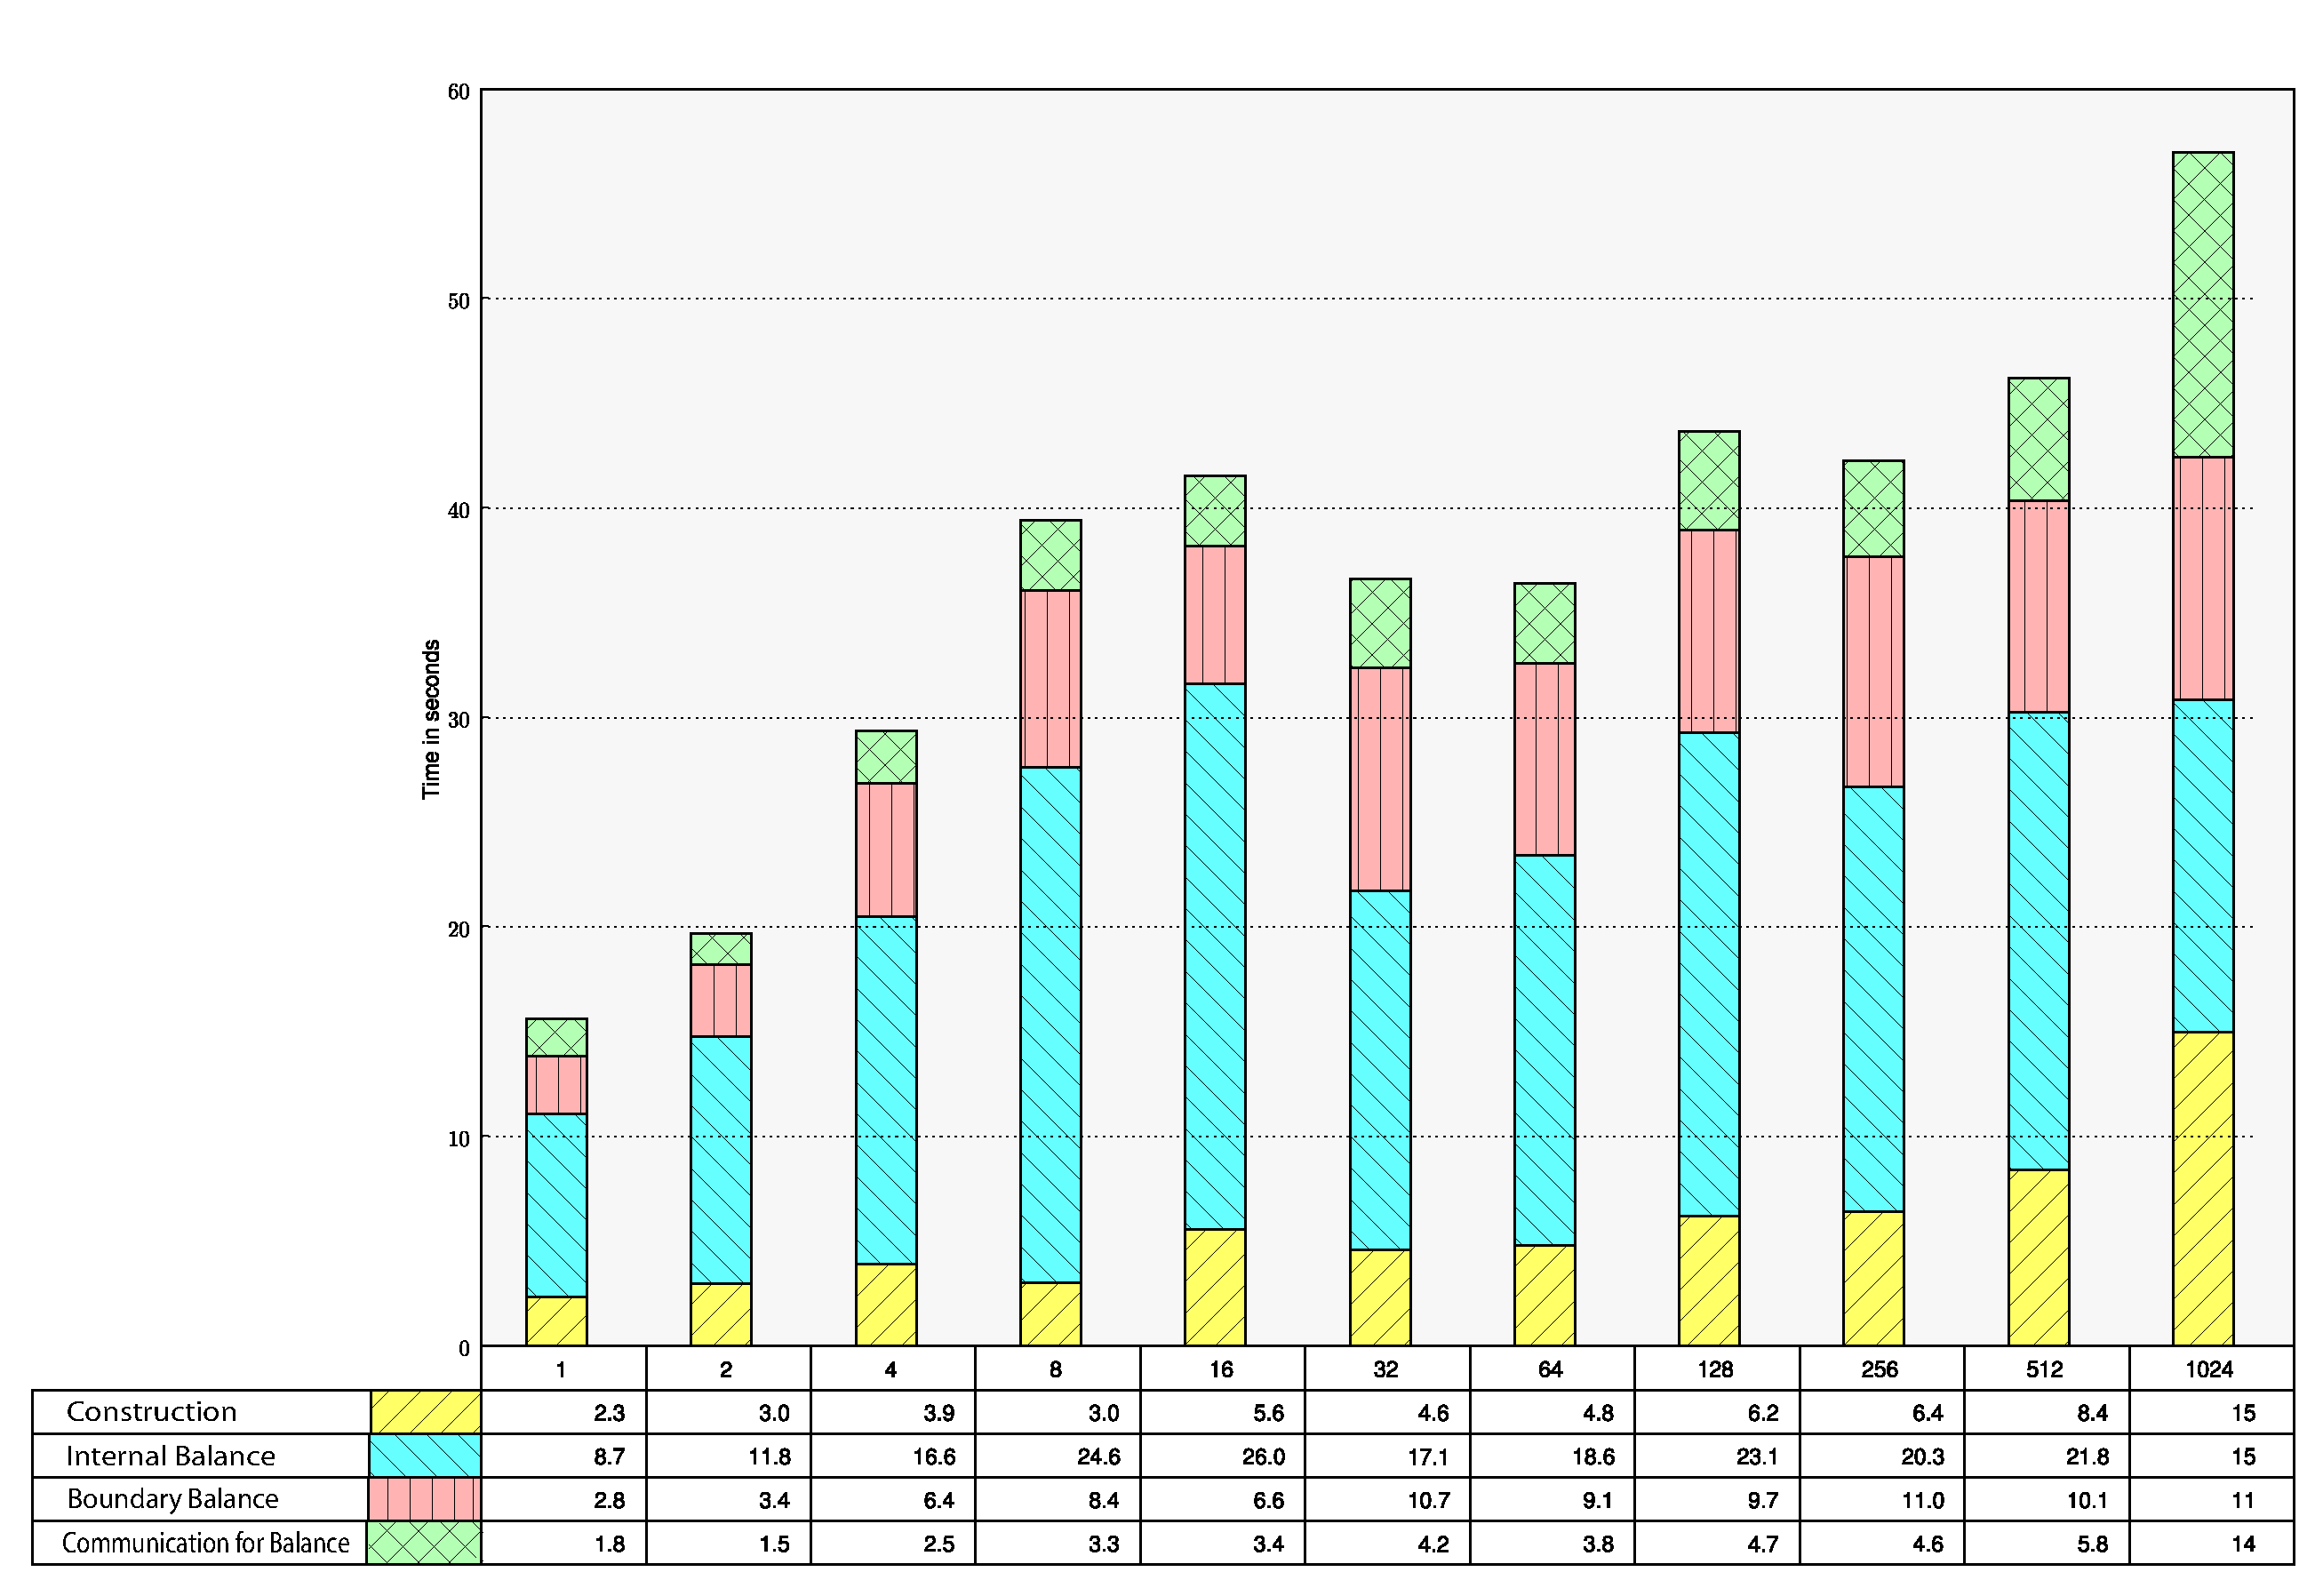
\includegraphics[width=\textwidth]{images/isoGran}
  \end{center}
  \caption{Isogranular scalability for Gaussian distribution of
  {\tt1M} octants per processor. From left to right, the bars indicate
  the time taken for the different components of our algorithms for
  increasing processor counts. The bar for each processor is
  partitioned into {\tt4} sections. From top to bottom, the sections
  represent the time taken for {\tt(1)} communication (including
  related pre-processing and post-processing) during balance
  refinement {\tt(Algorithm \ref{alg:parBal})}, {\tt(2)} balancing
  across intra and inter processor boundaries {\tt(Algorithm
  \ref{alg:ripple})}, {\tt(3)} balancing the blocks {\tt(Algorithm
  \ref{alg:effConBal})} and {\tt(4)} construction from points
  {\tt(Algorithm \ref{alg:p2o})}.}
  \label{fig:isoG}
\end{figure}

\begin{figure}
  \begin{center}
    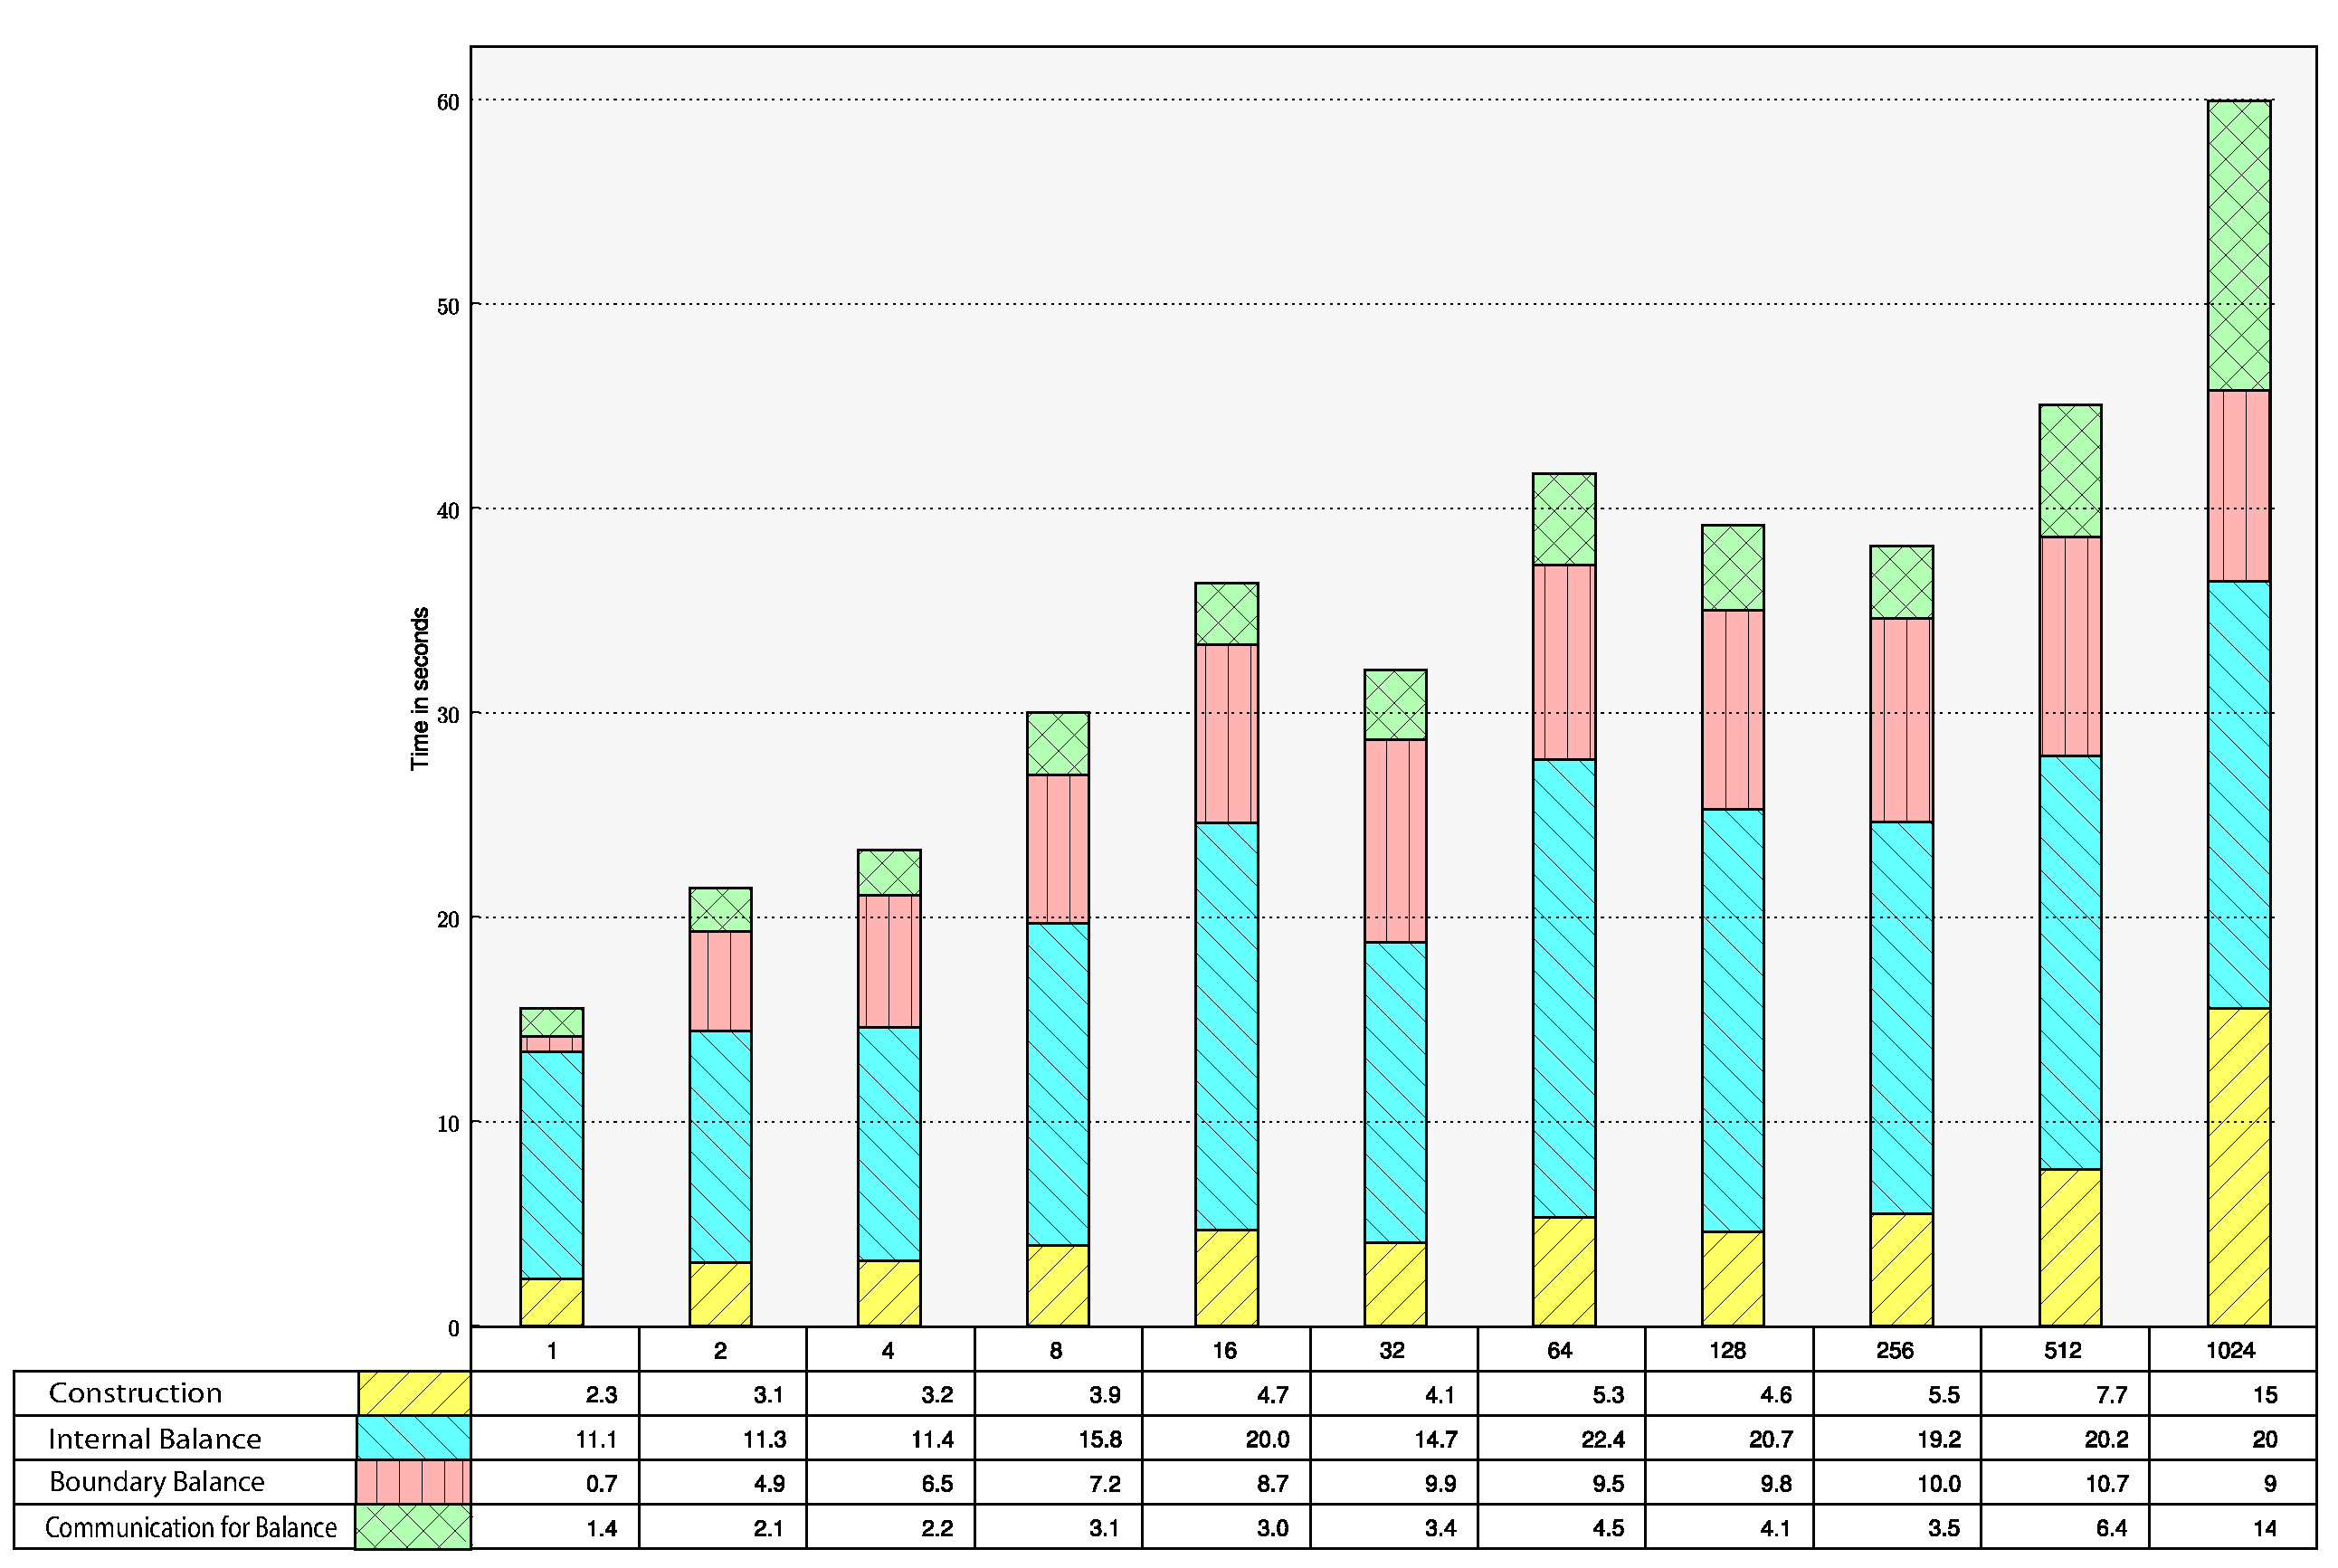
\includegraphics[width=\textwidth]{images/isoLN}
  \end{center}
  \caption{Isogranular scalability for Log-normal distribution of
  {\tt1M} octants per processor. From left to right, the bars indicate
  the time taken for the different components of our algorithms for
  increasing processor counts. The bar for each processor is
  partitioned into {\tt4} sections. From top to bottom, the sections
  represent the time taken for {\tt(1)} communication (including
  related pre-processing and post-processing) during balance
  refinement {\tt(Algorithm \ref{alg:parBal})}, {\tt(2)} balancing
  across intra and inter processor boundaries {\tt(Algorithm
  \ref{alg:ripple})}, {\tt(3)} balancing the blocks {\tt(Algorithm
  \ref{alg:effConBal})} and {\tt(4)} construction from points
  {\tt(Algorithm \ref{alg:p2o})}.}
  \label{fig:isoLN}
\end{figure}

\begin{figure}
  \begin{center}
    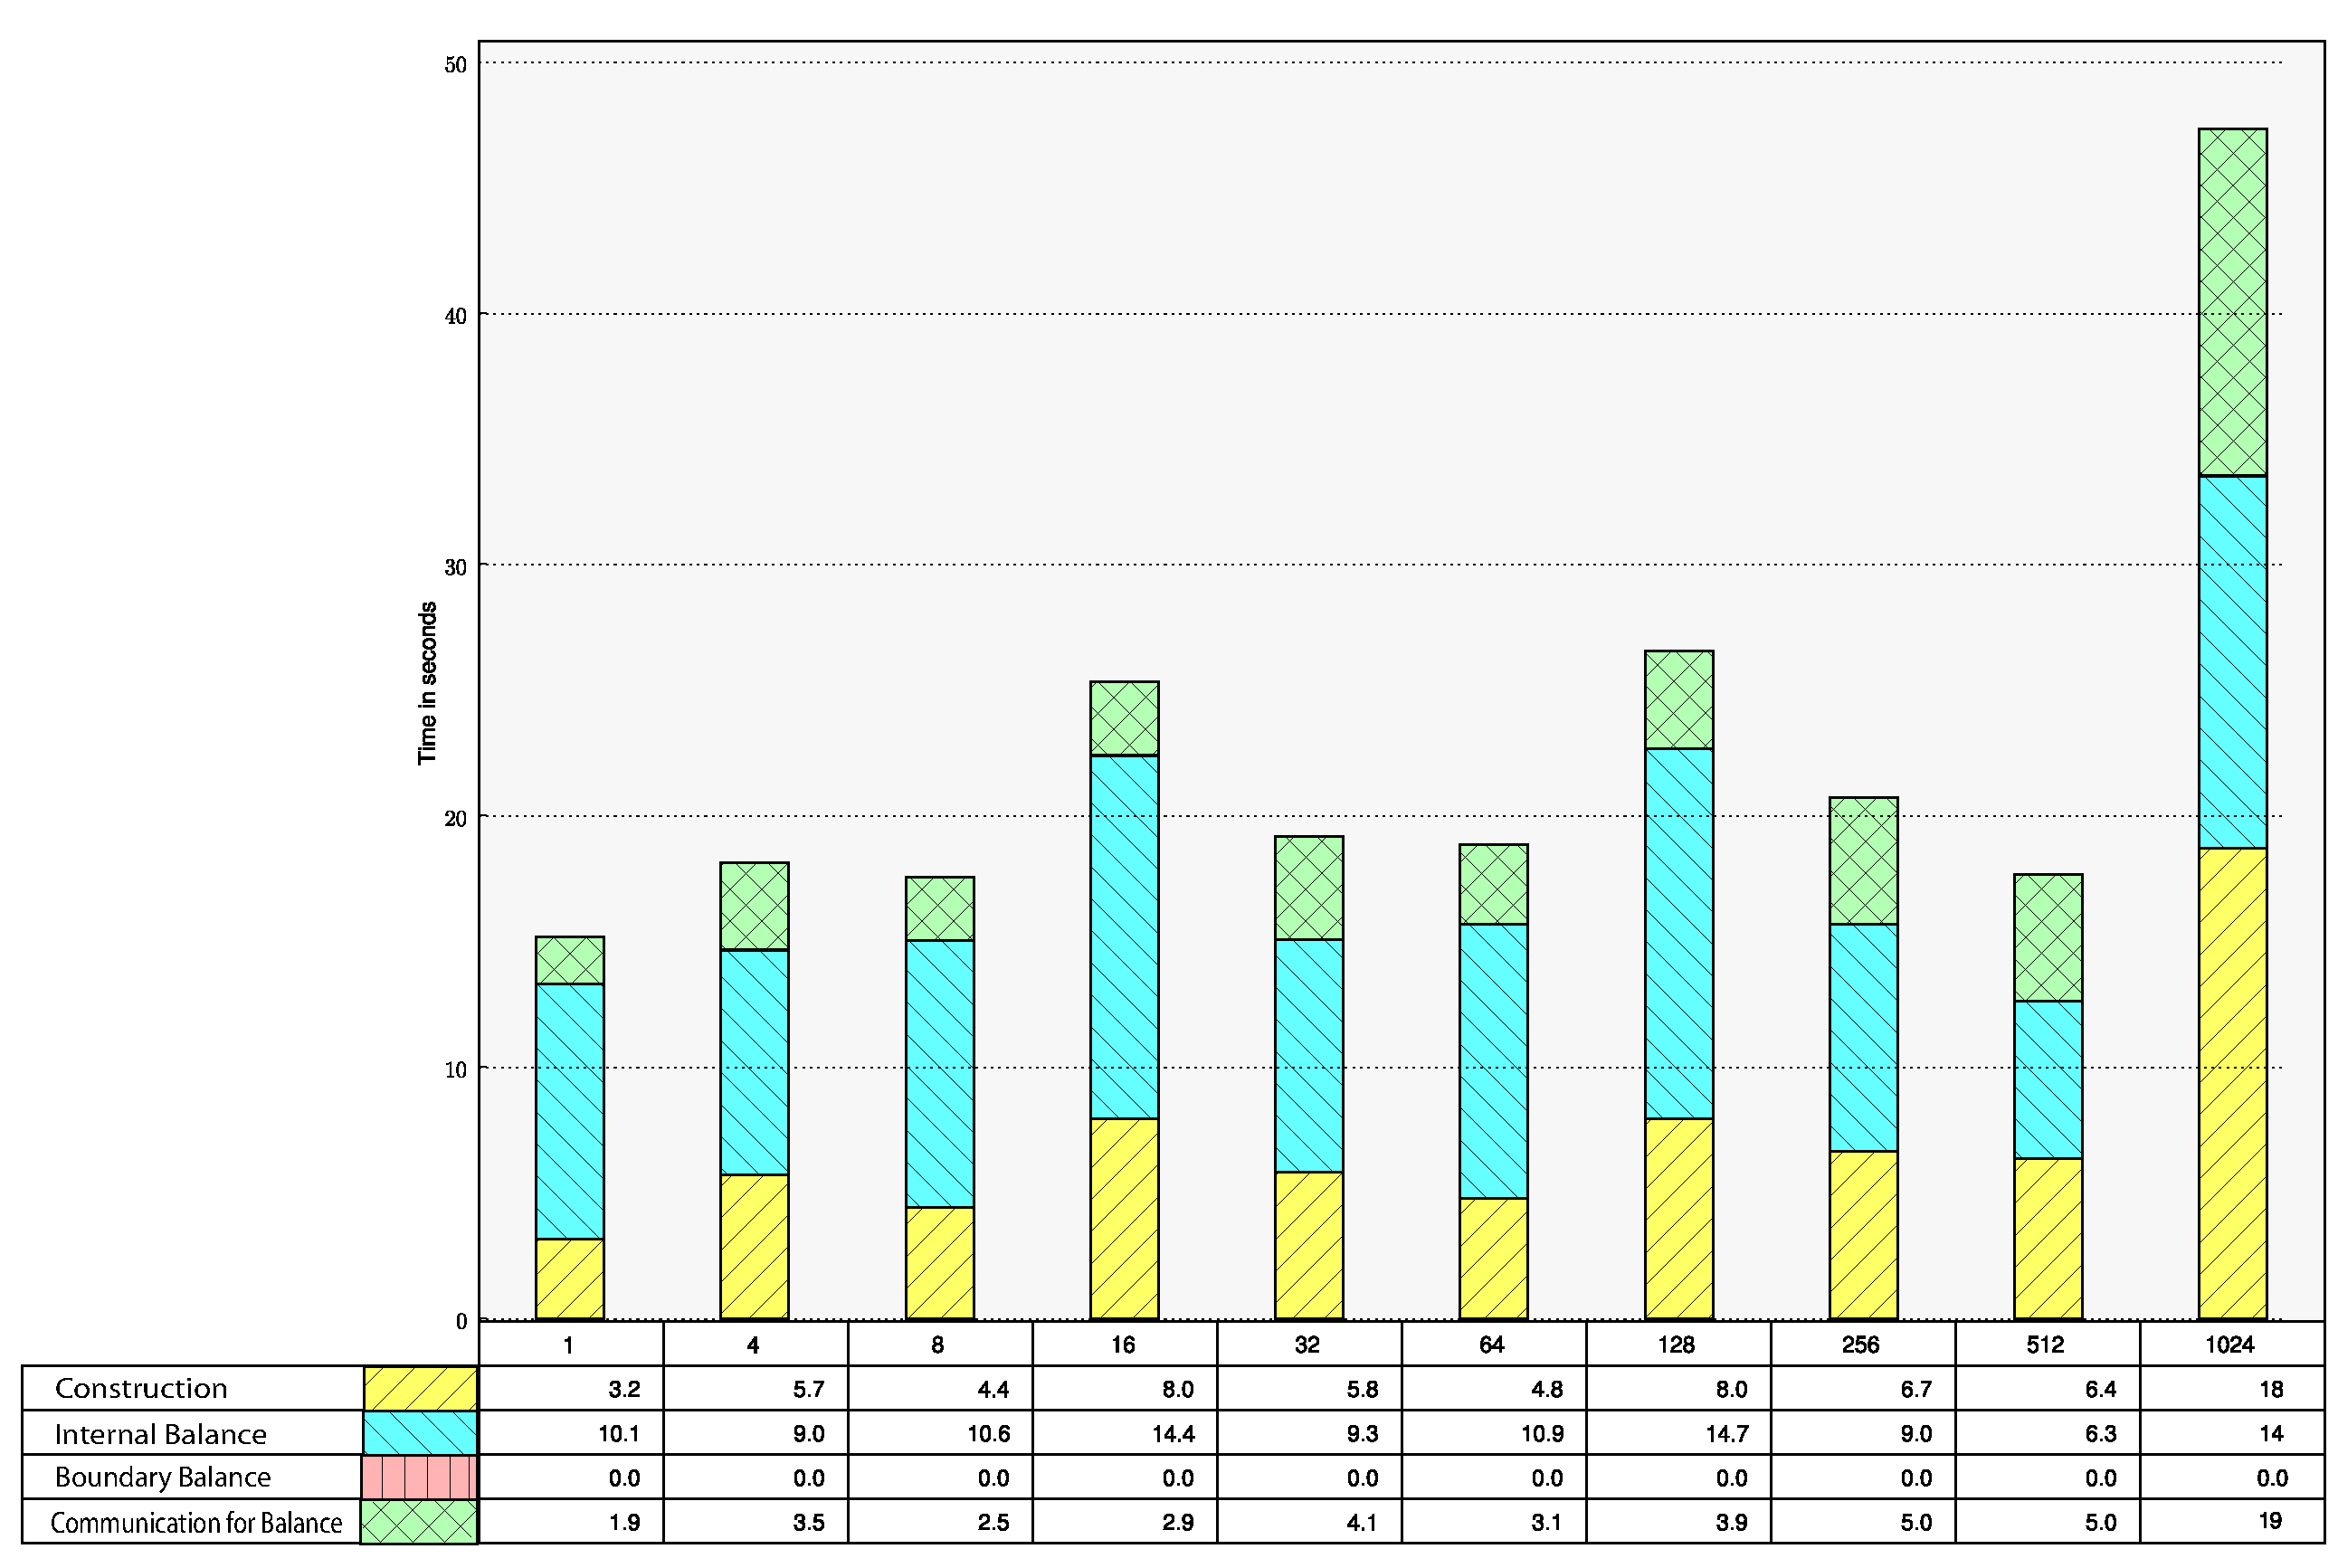
\includegraphics[width=\textwidth]{images/isoRG}
  \end{center}
  \caption{Isogranular scalability for uniformly spaced points with
  {\tt1M} octants per processor. From left to right, the bars indicate
  the time taken for the different components of our algorithms for
  increasing processor counts. The bar for each processor is
  partitioned into {\tt4} sections. From top to bottom, the sections
  represent the time taken for {\tt(1)} communication (including
  related pre-processing and post-processing) during balance
  refinement {\tt(Algorithm \ref{alg:parBal})}, {\tt(2)} balancing
  across intra and inter processor boundaries {\tt(Algorithm
  \ref{alg:ripple})}, {\tt(3)} balancing the blocks {\tt(Algorithm
  \ref{alg:effConBal})} and {\tt(4)} construction from points
  {\tt(Algorithm \ref{alg:p2o})}. While both the input and output
  grain sizes remain almost constant for the Gaussian and LogNormal
  distributions, only the output grain size remains constant for the
  Uniform distribution. Hence, the trend seen in this study is a
  little different from those for the Gaussian and LogNormal
  distributions.}
  \label{fig:isoRG}
\end{figure}

Fixed size scalability tests were also performed for three problem set
sizes, small (1 million points), medium (32 million points) and large
(128 million points), for the Gaussian distribution. These results are
plotted in Figures \ref{fig:fsS}, \ref{fig:fsM} and \ref{fig:fsL}.

\begin{figure}
  \begin{center}
    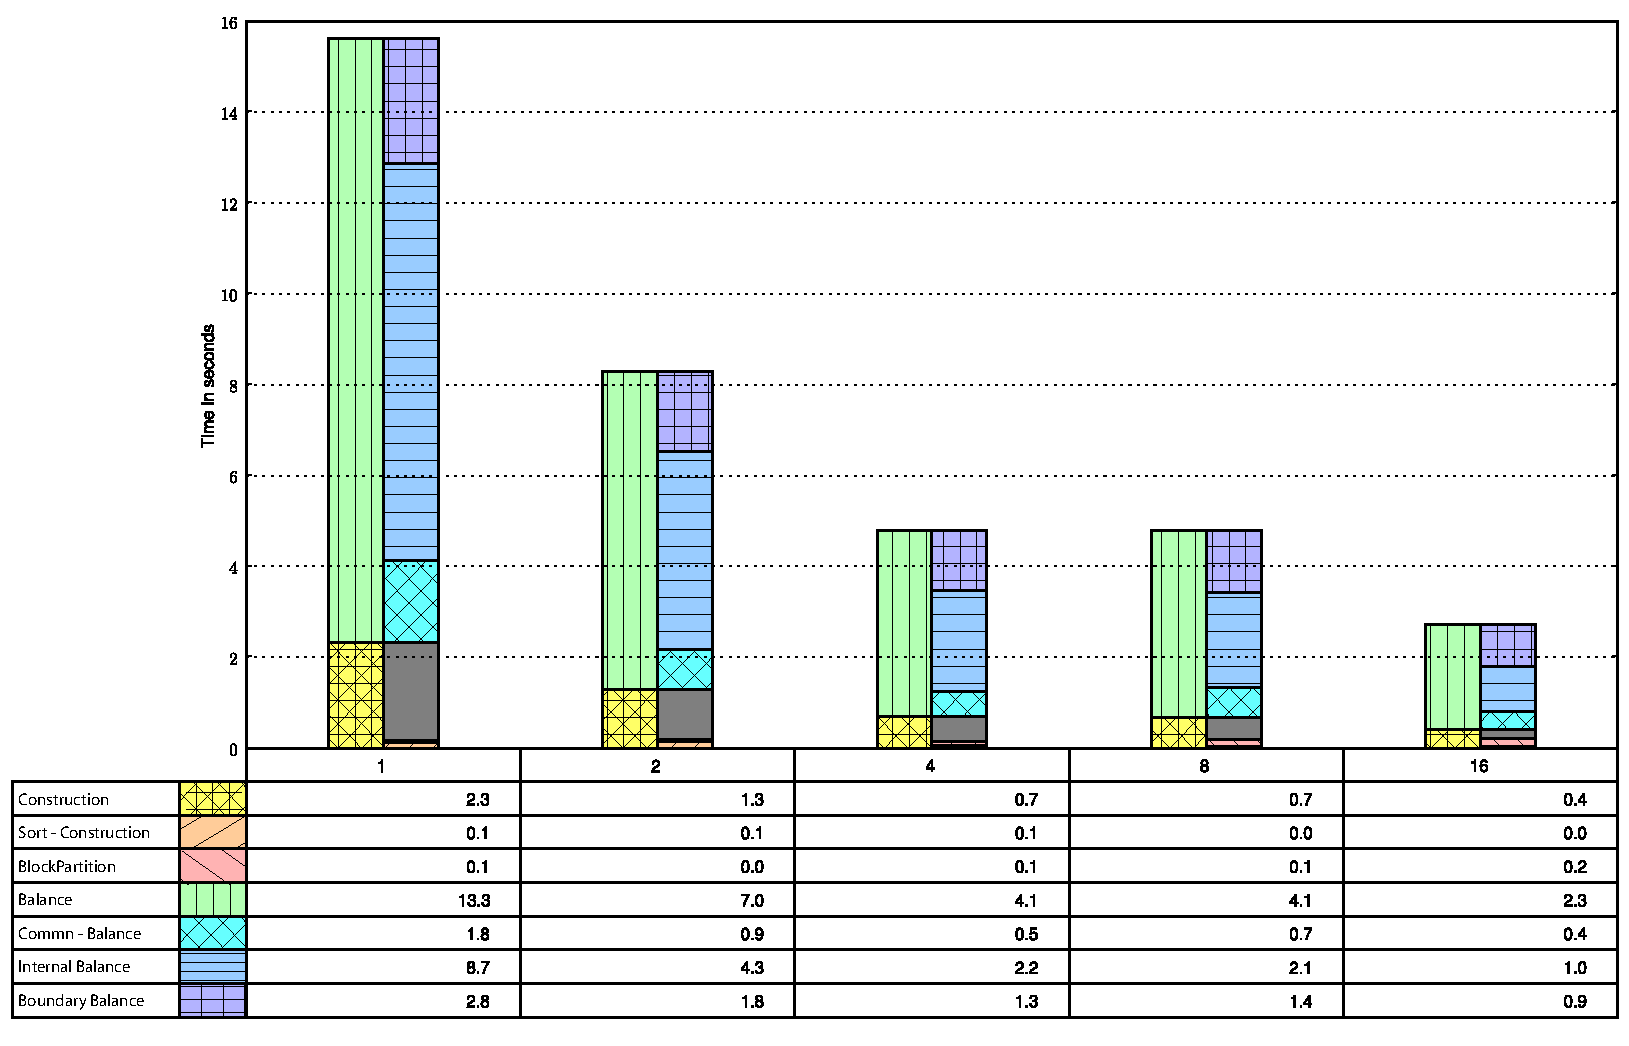
\includegraphics[width=0.9\textwidth]{images/fs1}
  \end{center}
  \caption{Fixed size scalability for Gaussian distribution of {\tt1M}
  octants. From left to right, the bars indicate the time taken for
  the different components of our algorithms for increasing processor
  counts. The bar for each processor is partitioned into {\tt2}
  columns, which are further subdivided. The left column is subdivided
  into {\tt2} sections and the right column is subdivided into {\tt6}
  sections. The top and bottom sections of the left column represent
  the total time taken for {\tt(1)} balance refinement {\tt(Algorithm
  \ref{alg:parBal})} and {\tt(2)} construction {\tt(Algorithm
  \ref{alg:p2o})}, respectively. From top to bottom, the sections of
  the right column represent the time taken for {\tt(1)} balancing
  across intra and inter processor boundaries {\tt(Algorithm
  \ref{alg:ripple})}, {\tt(2)} balancing the blocks {\tt(Algorithm
  \ref{alg:effConBal})}, {\tt(3)} communication (including related
  pre-processing and post-processing) during balance refinement,
  {\tt(4)} local processing during construction, {\tt(5)} {\tt
  BlockPartition} and {\tt(6)} {\tt Sample Sort}.}
  \label{fig:fsS}
\end{figure}

\begin{figure}
  \begin{center}
    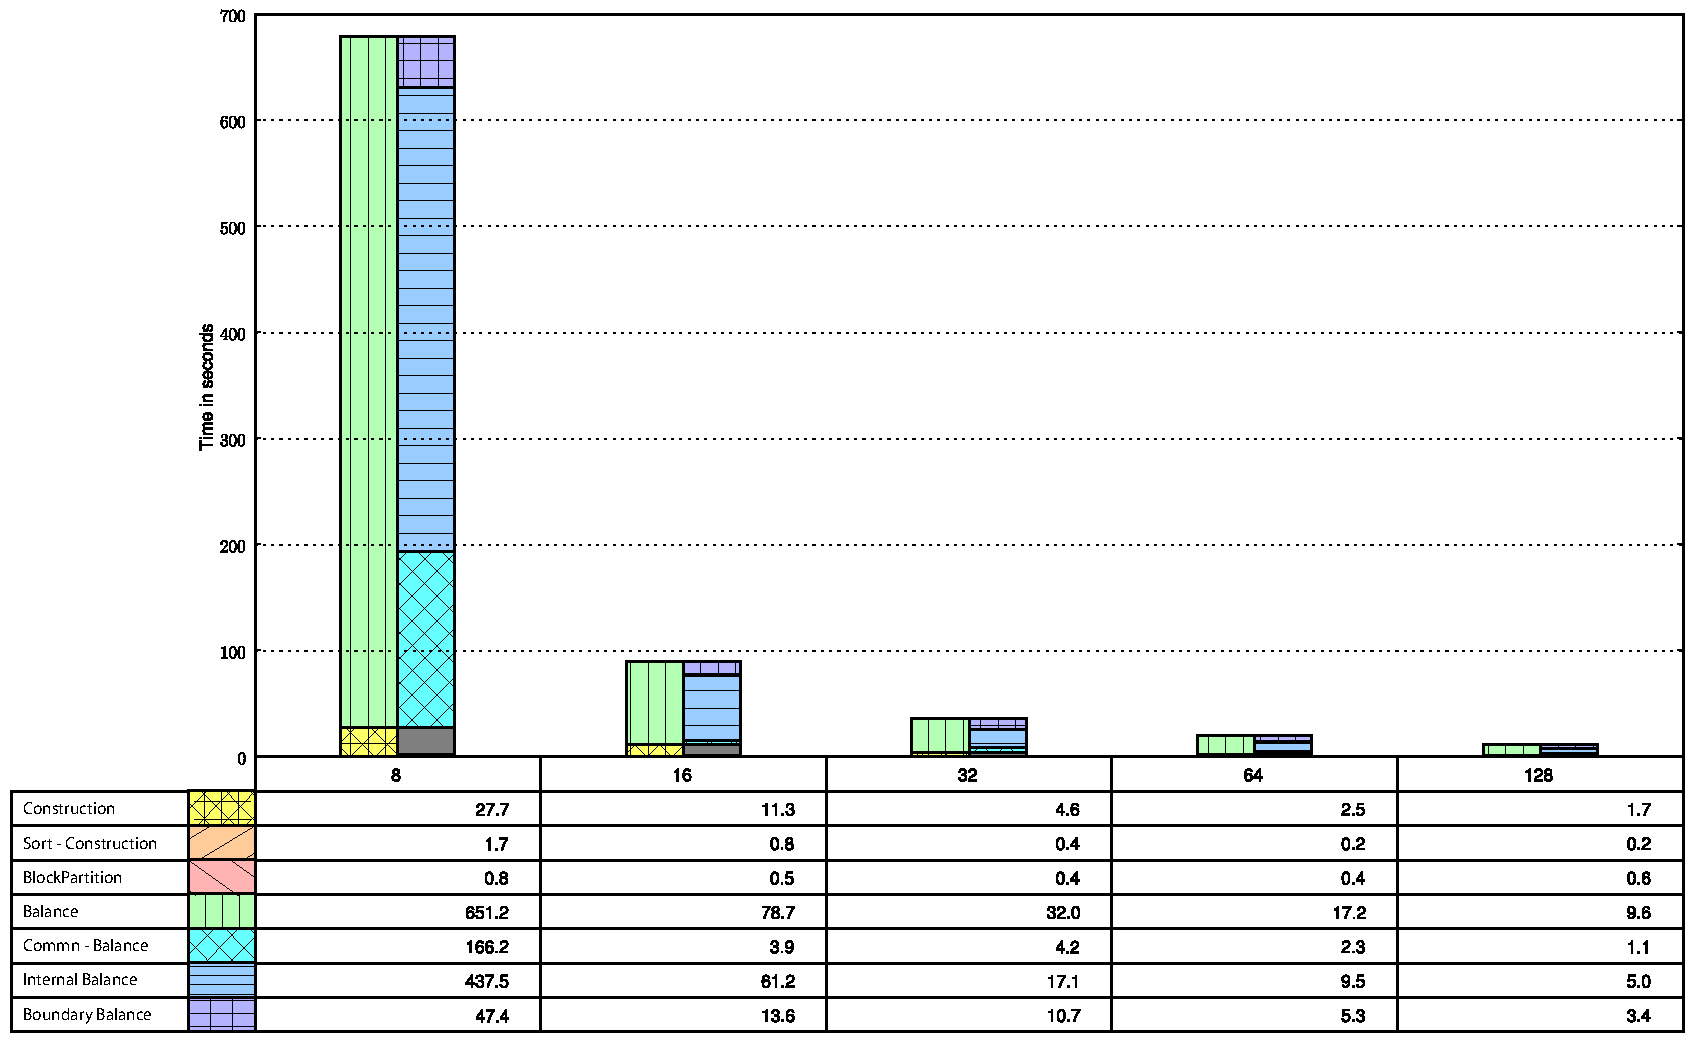
\includegraphics[width=0.9\textwidth]{images/fs32}
  \end{center}
  \caption{Fixed size scalability for Gaussian distribution of
  {\tt32M} octants. From left to right, the bars indicate the time
  taken for the different components of our algorithms for increasing
  processor counts. The bar for each processor is partitioned into
  {\tt2} columns, which are further subdivided. The left column is
  subdivided into {\tt2} sections and the right column is subdivided
  into {\tt6} sections. The top and bottom sections of the left column
  represent the total time taken for {\tt(1)} balance refinement
  {\tt(Algorithm \ref{alg:parBal})} and {\tt(2)} construction
  {\tt(Algorithm \ref{alg:p2o})}, respectively. From top to bottom,
  the sections of the right column represent the time taken for
  {\tt(1)} balancing across intra and inter processor boundaries
  {\tt(Algorithm \ref{alg:ripple})}, {\tt(2)} balancing the blocks
  {\tt(Algorithm \ref{alg:effConBal})}, {\tt(3)} communication
  (including related pre-processing and post-processing) during
  balance refinement, {\tt(4)} local processing during construction,
  {\tt(5)} {\tt BlockPartition} and {\tt(6)} {\tt Sample Sort}.}
  \label{fig:fsM}
\end{figure}

\begin{figure}
  \begin{center}
    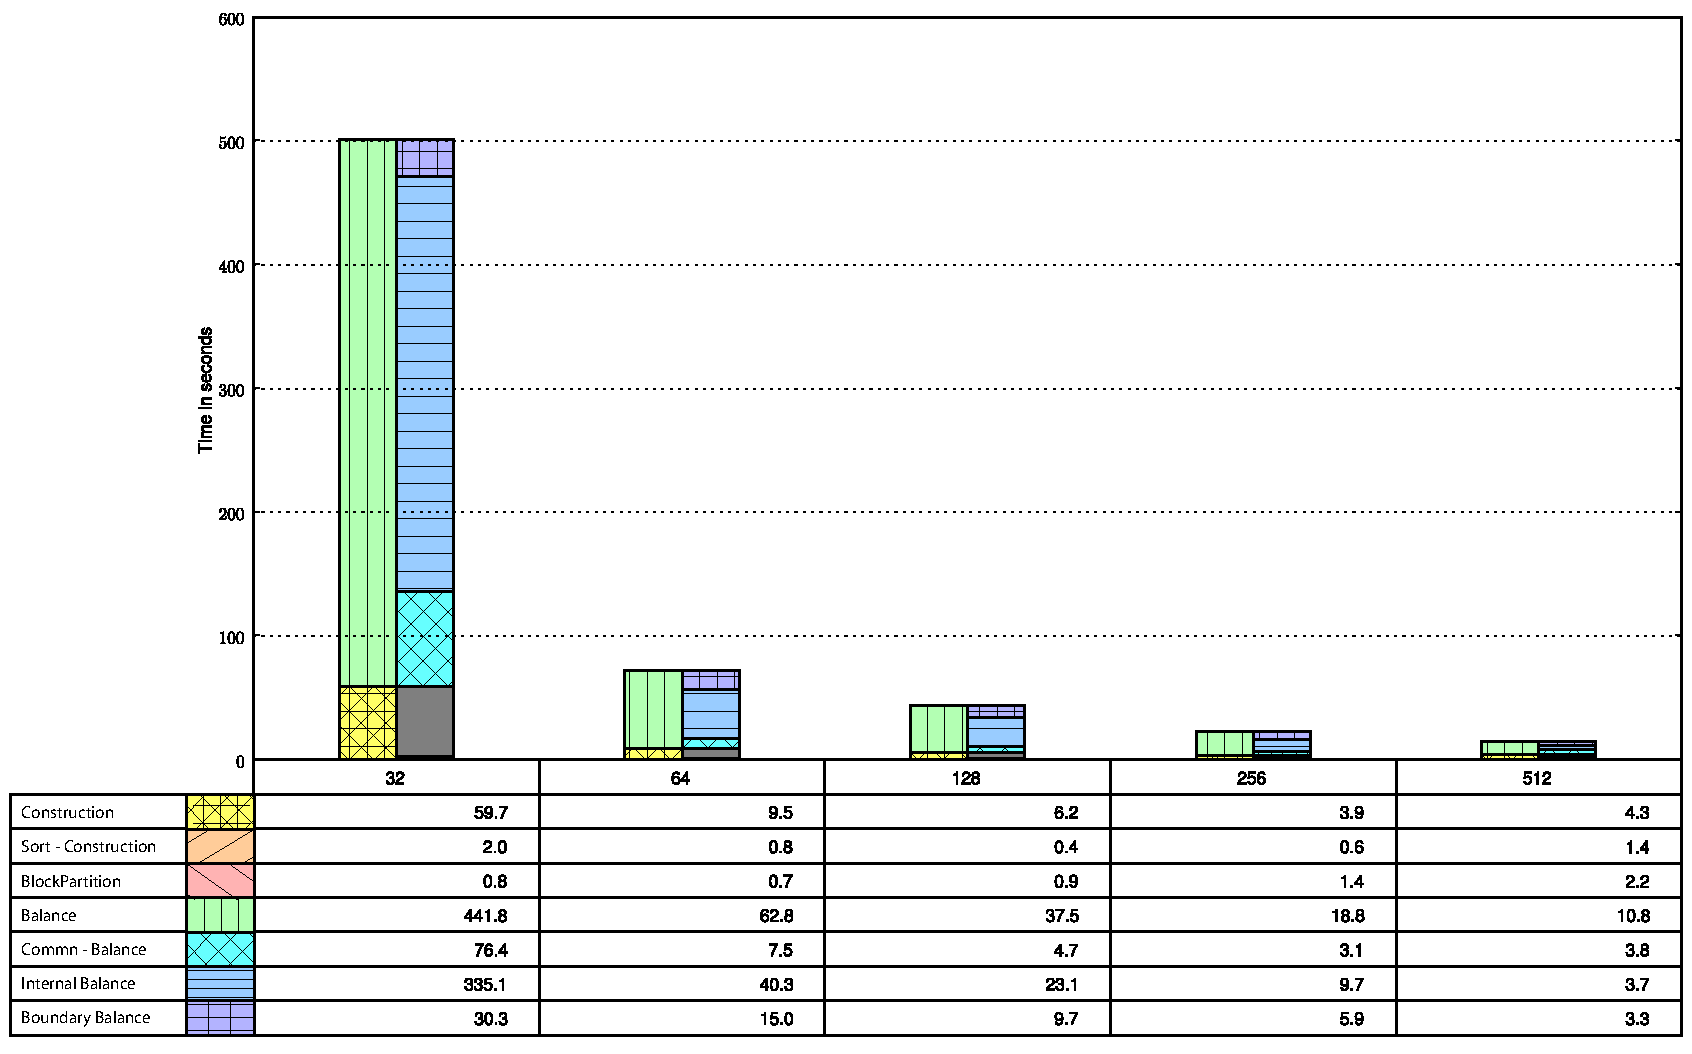
\includegraphics[width=0.9\textwidth]{images/fs128}
  \end{center}
  \caption{Fixed size scalability for Gaussian distribution of
  {\tt128M} octants. From left to right, the bars indicate the time
  taken for the different components of our algorithms for increasing
  processor counts. The bar for each processor is partitioned into
  {\tt2} columns, which are further subdivided. The left column is
  subdivided into {\tt2} sections and the right column is subdivided
  into {\tt6} sections. The top and bottom sections of the left column
  represent the total time taken for {\tt(1)} balance refinement
  {\tt(Algorithm \ref{alg:parBal})} and {\tt(2)} construction
  {\tt(Algorithm \ref{alg:p2o})}, respectively. From top to bottom,
  the sections of the right column represent the time taken for
  {\tt(1)} balancing across intra and inter processor boundaries
  {\tt(Algorithm \ref{alg:ripple})}, {\tt(2)} balancing the blocks
  {\tt(Algorithm \ref{alg:effConBal})}, {\tt(3)} communication
  (including related pre-processing and post-processing) during
  balance refinement, {\tt(4)} local processing during construction,
  {\tt(5)} {\tt BlockPartition} and {\tt(6)} {\tt Sample Sort}.}
  \label{fig:fsL}
\end{figure}

%}}}

%{{{ conclusions
\section{Conclusions}
\label{sec:conclude}
We have presented two new parallel algorithms for constructing and
balancing large linear octrees on distributed memory machines. We have
also tested MPI-based scalable parallel implementations for both the
algorithms.  Our algorithms have several important features:
\begin{itemize}
\item Experiments on three different types of input distributions
demonstrate that the algorithms are insensitive to the underlying data
distribution.
\item Our algorithms avoid iterative communications and thus are able
to achieve low absolute runtime and good scalability.
\item The experiments for comparing the performance of different
algorithms for the local balancing stage demonstrated that the one
proposed in this paper has a significantly lower running time than the
others.
\item We demonstrated scalability up to 1024 processors: we were able
to construct and balance octrees with over 1 billion octants in less
than a minute.
\end{itemize}

We need to consider the following factors to improve the performance
of the proposed algorithms. In order to minimize communication costs,
it is desirable to have as large coarse blocks as possible since the
communication cost is proportional to the area of the inter-processor
boundaries. However, too coarse blocks will increase the work for the
local block balancing stage (Section \ref{sec:conBal}). If additional
local splits are introduced, then the intra-block boundaries increase
causing the work load for the first ripple balance to increase. The
local balancing step of the algorithm can be made more efficient by
performing the local balancing recursively by estimating the correct
size of the block that can be balanced by the search-free
approach. Such an approach should be based on low-level architecture
details, like the cache size. %We intend to further improve the
%performance of our algorithms by adapting the algorithm to minimize
%cache misses.

%{{{ Morton encoding properties
\section{Properties of Morton encoding}
\label{app:prop}

\begin{prop}
Sorting all the leaves in the ascending order of their Morton ids is
identical to a preorder traversal of the leaves of the octree. If one
connects the centers of the leaves in this order, one can observe a
Z-pattern in the Cartesian space. The space-filling Z-order curve has
the property that spatially nearby octants tend to be clustered
together. The octants in Figures \ref{fig:completeOctree} and
\ref{fig:balancedOctree} are all labeled according to this
order. Depending on the order of interleaving the coordinates,
different Z-order curves are obtained. The two possible Z-curves in
2-D are shown in the Figure \ref{fig:ztypes}. Similarly, in 3-D six
different types of Morton ordering are possible.
  \label{ZdefProp}
\end{prop}

\begin{figure}
  \begin{center}
    \includegraphics[width=0.5\textwidth]{images/MortonZtypes}  
  \end{center}
  \caption{Two types of z-ordering in quadtrees.}
    \label{fig:ztypes}
\end{figure}

\begin{prop}
Given three octants, $a < b < c$ and $c \notin \{\mathcal{D}(b)\}$:
  \[
  a < d < c, ~~\forall d \in \{\mathcal{D}(b)\}.
  \]
  \label{prop:decFirst}
\end{prop}

\begin{prop}
The Morton id of any node is less than those of its descendants.
  \label{prop:ancLesser}
\end{prop}

\begin{prop}
Two distinct octants overlap if and only if one is an ancestor of the
other.
\label{prop:overlap}
\end{prop}

\begin{prop}
The Morton id of any node and of its first child\footnote{the child
that has the same anchor as the parent} are consecutive. It follows
from Property \ref{prop:ancLesser} that the first child is also the
child with the least Morton id.
  \label{prop:fcProp}
\end{prop}

\begin{prop}
The first descendant at level $l$, denoted by
$\mathcal{FD}\left(N,l\right)$, of any node $N$ is the descendant at
level $l$ with the least Morton id. This can be arrived at by
following the first child at every level starting from
$N$. $\mathcal{FD}\left(N,D_{max}\right)$ is also the anchor of $N$
and is also referred to as the {\em deepest first descendant}, denoted
by $\mathcal{DFD}(N)$, of node $N$.
  \label{prop:fdProp}
\end{prop}

\begin{prop}
The range $(N,\mathcal{DFD}(N)]$ only contains the first descendants
of $N$ at different levels and hence there can be no more than one
leaf in this range in the entire linear octree.
  \label{prop:rangeFprop}
\end{prop}

\begin{prop}
The {\em last descendant} at level $l$, denoted by
$\mathcal{LD}\left(N,l\right)$, of any node $N$ is the descendant at
level $l$ with the greatest Morton id. This can be arrived at by
following the {\em last child}\footnote{child with the greatest Morton
id} at every level starting from
$N$. $\mathcal{LD}\left(N,D_{max}\right)$ is also referred to as the
{\em deepest last descendant}, denoted by $\mathcal{DLD}(N)$, of node
$N$.
  \label{prop:ldProp}
\end{prop}

\begin{prop}
Every octant in the range $(N,\mathcal{DLD}(N)]$ is a descendant of
$N$.
  \label{prop:rangeLprop}
\end{prop}
%}}}

%{{{ Multicomponent representation
\section{Multicomponent Morton Representation}
\label{app:mortonClass}
Every Morton id is a set of 4 entities: The three co-ordinates of the
anchor of the octant and the level of the octant. We have implemented
the node as a C++ class, which contains these 4 entities as its member
data. To use this set as a locational code for octants, we define two
primary binary logical operations on it: a) Comparing if 2 ids are
equal and b) Comparing if one id is lesser than the other.

Two ids are equal if and only if all the 4 entities are respectively
equal. If two ids have the same anchor then the one at a coarser level
has a lesser Morton id. If the anchors are different, then we can use
Algorithm \ref{alg:lessOp} to determine the lesser id. The Z-ordering
produced by this operator is identical to that produced by the scalar
Morton ids described in section \ref{sec:morton}. The other logical
operations can be readily derived from these two operations.


\begin{table*}
\centering
\rule{\textwidth}{0.01mm}
\begin{algorithm}{ \textsc{Finding the lesser of two Morton ids (sequential)}}
\rule{\textwidth}{0.01mm}
\flushleft
\tt{\bf{Input:~} Two Morton ids, $A$ and $B$ with different anchors.} \\
\tt{\bf{Output:} $R,$ the lesser of the two Morton ids.}\\
~\\
1. $X_i \leftarrow \left(A_i \oplus B_i\right)$, $i \in \{x, y, z\}$\\
2. $e \leftarrow \argmax{i} (\lfloor\log_2(X_i)\rfloor)$ \\
\begin{tabbing}
3. {\bf if} \= $A_e < B_e$ \\
           \> $R \leftarrow A$\\
4. {\bf else} \\
             \>  $R \leftarrow B$\\
5. {\bf end if}
\end{tabbing}
\label{alg:lessOp}
\end{algorithm}
\rule{\textwidth}{0.01mm}
\end{table*}
%}}}

%{{{ Block partitionings
\section{Analysis of the Block Partitioning Algorithm}
\label{app:blkPartAnal}
Assume that the input to the partitioning algorithm is a sorted
distributed list of $N$ octants. Then, we can guarantee coarsening of
the input if there are more than {\tt8} octants\footnote{$2^d$ cells
for a $d$-tree.} per processor. The minimum number of octants on any
processor, $n_{min},$ can be expressed in terms of $N$ and the
imbalance factor\footnote{The imbalance factor is the ratio between
the maximum and minimum number of octants on any processor.}, $c,$ as
follows:
\[
n_{min} = \frac{N}{1+c(n_p-1)}.
\]

This implies that the coarsening algorithm will coarsen the octree if,
\begin{eqnarray*}
n_{min} = \frac{N}{1+c(n_p-1)} & > & 2^d, \\
\implies N > 2^d(1 + c(n_p - 1)).
\end{eqnarray*}

The total number of blocks created by our coarsening algorithm is
$\mathcal{O}(p)$. Specifically, the total number of blocks produced by
the coarsening algorithm, $N_{blocks}$, satisfies:
\[
p \le N_{blocks} < 2^d p.
\]

If the input is sorted and if $c \approx 1$, then the communication
cost for this partition is $\mathcal{O}(\frac{N}{n_p})$.
%}}}

%{{{ Special case while constructiong
\section{Special case during construction}
\label{app:specialCon}
We can not always guarantee the coarsest possible octree for an
arbitrary distribution of $N$ points and arbitrary values of
$N^p_{max}$, especially when $N^p_{max} \approx
\frac{N}{n_p}$. However, if every processor has at least 2
{\em{well-separated}} \footnote{Convert the points into octants at
$D_{max}$ level. If there exists at least one coarse octant between
these two octants, then the points are considered to be
well-separated.} points and if $N^p_{max}=1$, then the algorithm will
produce the coarsest possible octree under these constraints.
However, this is not too restrictive because the input points can
always be sampled in such a way that the algorithm produces the
desired octree. Besides, the maximum depth of the octree can also be
used to control the coarseness of the resulting octree. In all our
experiments, we used $N^p_{max}=1$ and we always got the same octree
for different number of processor counts (Table \ref{tab:numbers}).
%}}}


\chapter{Inverse Problem}
\label{chap:inverse}
\include {results}	     

% And the bibliography

\bibliographystyle{plain}
\bibliography{thesis,octree}

\end{document}

